% -*- mode: latex-mode; TeX-engine: xetex; LaTeX-command-style: (("" "SOURCE_DATE_EPOCH=0 %(PDF)%(latex) --shell-escape %S%(PDFout)")); -*-

\documentclass{Dissertate}

\usepackage{fltpage2}

\newcommand{\todo}[1]{}

\begin{document}

% Formatting guidelines found in:
% http://www.gsas.harvard.edu/publications/form_of_the_phd_dissertation.php
% -*- mode: latex-mode; TeX-engine: xetex; LaTeX-command-style: (("" "SOURCE_DATE_EPOCH=0 %(PDF)%(latex) --shell-escape %S%(PDFout)")); TeX-master: "../dissertation.tex"; -*-

% Some details about the dissertation.
\title{Coherent Association of Single Molecules from Single Atoms}
\author{Yichao Yu}

%If you have one advisor
\advisor{Kang-Kuen Ni}

% \committeeInternalOne{Person Inside One}
% \committeeInternalTwo{Person Inside Two}
% \committeeExternal{Person Outside}

% ... about the degree.
\degree{Doctor of Philosophy}
\field{Physics}
\degreeyear{2021}
\degreeterm{Winter}
\degreemonth{March}
\department{Physics}

% ... about the candidate's previous degrees.
\pdOneName{B.S.}
\pdOneSchool{Massachusetts Institute of Technology}
\pdOneYear{2014}

\makeatletter
\hypersetup{
  pdfauthor={\@author},
  pdftitle={\@title},
  pdfsubject={Ph.D Thesis},
  pdfkeywords={Physics, AMO, Laser, Atomic Physics, Molecular Physics, Optics,
  Ultracold, Ultracold Atoms, Ultracold Molecules, Diatomic Molecules,
  Sodium, Cesium, NaCs, Coherent Transfer, Single Atoms, Single Molecule, Optical Tweezer,
  Molecule Assembly, Raman Transition, STIRAP, Raman Sideband Cooling,
  Photoassociation, Computer Control, LLVM, FPGA}
}
\makeatother

\maketitle
\copyrightpage
\abstractpage{% -*- mode: latex-mode; TeX-engine: xetex; LaTeX-command-style: (("" "SOURCE_DATE_EPOCH=0 %(PDF)%(latex) --shell-escape %S%(PDFout)")); TeX-master: "../dissertation.tex"; -*-

%% the abstract
Neutral molecules, with their rich spectrum of internal states as well as
strong and tunable dipolar interactions, are promising candidates for
a broad range of experiments including quantum information,
quantum chemistry, precision measurement and probing of beyond-Standard-Model physics,
and quantum simulation of interacting many-body systems.
At the same time, the complexity that made them attractive also poses a significant challenge
to achieve a high level of quantum control that is required in many of
their potential applications.
Multiple approaches are being pursued for full quantum control of molecules
including association of atomic gases and direct cooling of molecules,
yet it remains challenging to control molecules at single particle level
due to the difficulty in tuning the atom-atom interaction
and laser cooling of molecules.

\todo{
  In this thesis, we successfully achieved full quantum control
  on a stable weakly bound molecule associated via optical transfer from atoms.
  use optical tweezer to achieve control
  optical tweezers also allows scaling up.
  Studied various interaction and molecule properties.
}
}
\contentspage
% \listoffigures % optional
\dedicationpage{% -*- mode: latex-mode; TeX-engine: xetex; LaTeX-command-style: (("" "SOURCE_DATE_EPOCH=0 %(PDF)%(latex) --shell-escape %S%(PDFout)")); TeX-master: "../dissertation.tex"; -*-

%% dedication text
}
\acknowledgments{% -*- mode: latex; TeX-engine: xetex; LaTeX-command-style: (("" "SOURCE_DATE_EPOCH=0 %(PDF)%(latex) --shell-escape %S%(PDFout)")); TeX-master: "../dissertation.tex"; -*-

%% the acknowledgments section

\todo{
  Advisor
  Lab members + Till
  CUA
  Undergrad lab members and advisor
  Family and friends
}
\todo{
  inline:
  Olivier for coupling to ground state continuum idea.
  Jeremy Hudson for calculation
  Bo Gao?
}
}
\setstretch{\dnormalspacing}

% include each chapter...
\setcounter{chapter}{-1}  % start chapter numbering at 0
% -*- mode: latex-mode; TeX-engine: xetex; LaTeX-command-style: (("" "SOURCE_DATE_EPOCH=0 %(PDF)%(latex) --shell-escape %S%(PDFout)")); TeX-master: "../dissertation.tex"; -*-

\chapter{Introduction}
\label{ch:introduction}

\section{Ultracold Molecules}
\label{ch:introduction:molecules}

Started with precise optical spectroscopy and the development of laser cooling
and trapping technologies, the increasing measurement precision and
high level of control has been one of the the primary driving forces
in the field of atomic physics in the past decades.
Systems based on cooling and controlling of neutral atoms
have been used in a wide range of applications including
quantum computing, quantum communication, precision measurement,
quantum simulation and the study of many other many body effects.

Despite these great successes, the utility of atom based systems
are limited by their simple internal structure and weak interactions.
Molecules, on the other hand, with its richer internal degrees of freedom
including electronic orbital, electron spin, neuclear vibration, rotation and spin,
the potential of stronger interaction and more variance of symmetry classes,
are better candidates for more applications especially in
quantum computing, precision measurement and quantum simulation.
Moreover, comparing to other systems with stronger interaction like ions and Rydberg atoms,
the interacting states in molecules are long lived and tunable thanks to
the abundance of low energy excitations,
which can offer better isolation from the environment giving rise to longer coherence time.

Many applications of molecules requires cooling and high level of control
on the quantum state of the molecules.
Unfortunately, the properties that makes molecules attractive
also makes controlling them harder.
The enabling technique for most ultracold atom experiment, laser cooling,
typically requires scattering of a large number of photons ($\approx10^4\sim10^7$).
This is possible in atomic system due to the existence of cycling transition
or near cycling ones that can be completely closed with
one or two spin states repumping lasers.
However, the lack of selection rules for vibrational states means that
such transition generally does not exist in molecules.
As a result, experiments aiming to achieve control of molecule on a similar level with atoms
usually take one of the two approaches,
\begin{enumerate}
\item Direct laser cooling of special molecules
  with approximate cycling transitions\todo{cite}.\\
  These are molecules that have optical transitions that has a high probability
  of decaying down to the same vibrational states.
  With the help of a few vibrational repumping lasers,
  scattering of $\approx10^3\sim10^5$ photons\todo{cite} can be achieved.
  Significant progress has been made using this approach in recent years
  including sub-doppler cooling and trapping of molecules in optical tweezers\todo{cite}.
  The main challenge with this approach is to achieve a better cooling performance
  given the still limitted photon scattering budget.
\item Creating of molecules from ultracold atoms.\\
  First realized a decade ago\cite{ni_high_2008}\todo{another cite},
  this approach takes advantage of the mature cooling and trapping techniques
  developped for atoms and creates molecules from atoms
  that are cooled to ultracold temperature.
  The difficulty with this approach is understandably in the creation of the molecule,
  which must be done with acceptable efficiency and coherence
  in order to maintain the cooling and controling done on the atoms.
  This approach currently allows a lower temperature to be achieved\todo{cite}
  and this is the approach used in our experiment.
\end{enumerate}

\section{Assembly of Molecules in Optical Tweezers}
\label{ch:introduction:tweezers}

Previous experiments that takes the approach to create ultracold molecules
from ultracold atoms do so either in a bulk gases or an optical lattice.
In these systems, however, the transfer efficiency and
the density of the created molecules are limited
by the overlap between the distribution of the two atomic speices.
Such overlap is controlled by the combination of the trapping potential
and the intra- and inter-species interactions.
Thus, a perfect overlap for molecule formation can only be achieved by fine tuning
the delicate balance between these parameters and may not always be possible.
Additionally, the molecules created in such matter may collide
with residue atoms or other molecules causing rapid loss
either through chemical reactions or by forming long-lived sticky complex.

Since these issues are essentially all caused by the lack of direct control
on the position and motion of individual atoms and molecules,
we propose a general solution using optical tweezers.
Created by focusing the trap light through a high numerical aperture~(NA) objective,
optical tweezers can trap single atoms in flexible geometry
and the setup naturally provides the high resolution required
for detection and manipulation of individual atoms.
Taking advantage of these properties, full quantum control on atoms has been demostrated
by cooling and rearranging the tweezer based on the loading result.
This gives us a good starting point to deterministically create molecules
by directly merging pairs of atoms instead of
relying on stochastic process or the fine tuning of parameters in previous experiments.
The molecules created using this approach are also well isolated from each other,
preventing loss due to collisions.

\todo{
  In additional to motional control, the confinement of the tweezer
  also decreases the distance between the atoms and thus increases the coupling
  between the atomic state and the molecular state.
  % all optical
}

The molecule we use to implement this approach is NaCs.
The Na and Cs froming the molecule can be cooled and manipulated
using many existing techniques developped for alkali atoms.
The molecule is also predicted to have a large
molecular fixed-frame dipole moments~($4.6~\mathrm{Debye}$)
in the singlet rovibrational ground state,\todo{figure about dipole moment}
making it a good candidate to demostrate interaction and entanglement
after created in the tweezers.
Nevertheless, we believe this approach is not limitted to our choice of molecule,
but can be applied to other molecules created from two atoms that can be laser cooled.

\todo{figure for steps}
The steps we propose to create the molecules in the tweezer are as follows,
\begin{enumerate}
\item Loading and cooling of single atoms in the tweezers.\\
  This is the step that give us the full quantum control on the atoms
  which will be translated to the control on the molecules later.
  Image of the atoms taken in this step can be used to rearrange the tweezers
  to acheive high filling fraction.
\item Merging of the atoms into a single tweezer.\\
  Using the precise control of the atoms from optical tweezers,
  we can merge a single Na and Cs that is trapped and cooled in separate tweezers
  into a single one deterministically.
\item Creation of weakly bound molecule and rovibrational ground state molecule.\\
  In order to create the rovibrational ground state molecules from atoms,
  we must remove the $\approx100~\mathrm{THz}$ binding energy coherently from the system,
  which is typically done using a two-photon optical transition.
  However, due to the significant mismatch in the wavefunction size
  between the atomic motional ground state~($\approx1000\text{\AA}$)
  and the rovibrational ground state of the molecule~($\approx4\text{\AA}$),
  it is challenging to achieve a high transition strength,
  causing technical difficulties in maintaining the laser coherence during the transition.
  In order to work around this problem,
  the association is done by first creating a weakly bound molecule,
  where the small energy difference makes it easier to maintain laser coherence,
  and then transfering to the final state,
  which has stronger coupling and shorter transition time.
\end{enumerate}

\section{Contents of this Thesis}
\label{ch:introduction:contents}

In this thesis, we describe the method we use to create a weakly bound ground state molecule
in the optical tweezer and the results leading up to it including the control of atoms
and the measurement on the interaction between the atoms and the molecular potential.

We start with chapter \ref{ch:computer-control} by giving a high level description of
the custom computer control system we use.
This system controls the timing of all the hardware outputs in the experiment
and is used to perform all the measurements in the rest of this thesis.

Chapter \ref{ch:loading} discusses the loading of the single atoms into the optical tweezer.
The discussion includes the preparation steps needed before the loading,
e.g. freespace cooling of atoms,
and the imaging of the atom in the tweezer,
which is the primary detection method used in our experiment.
All the experiments in the following chapters are performed using
the atoms and molecules in the optical tweezers.

Chapter \ref{ch:rsc} describes the Raman sideband cooling (RSC) process
we used to cool single Na atom in the optical tweezer.
As the lighter atom with a broader optical linewidth,
the RSC of Na atom faces additional challenges compared to atoms
that were cooled using similar method previously
and the tool we developed to overcome these challenges can be applied to other systems as well.

After preparation of the atomic state,
chapter \ref{ch:interaction-shift} starts our investigation of the interaction between atoms
by measuring the $s$-wave scattering length using interaction shift spectroscopy.
The measurement result is used to refine the prediction for Feshbach resonance
between Na and Cs atoms and also to improve the atomic state preparation.

Chapter \ref{ch:pa} discusses the measurement of the molecular excited states
by photoassociation spectroscopy.
We also study the effect of the tweezer beam on the molecular states and transitions.
The states mapped out in this measurement are used as intermediate states
to study the groud molecular states via two-photon transitions.

Following the previous chapter, chapter \ref{ch:raman-spectroscopy} discusses
the properties of the weakly bound ground molecular states using Raman spectroscopy.
We demostrated the ability to control the rotational states of the molecule
and studies the coupling of the molecule with external field
and the their hyperfine structure in the weakly bound regime.
The measurement identifies candidate target states for our coherent molecule creation.

Chapter \ref{ch:raman-transfer} combines the preparation and characterization
in the previous chapters and describes our all-optical coherent molecule formation process.
A detailed comparison between different approaches and states selection is given
to support our choice of experimental parameters.
We show our result on the coherent transfer and characterizes
the molecule we create as well as the transfer process.
We study the limit on the transfer efficiency
and list open questions in the transfer process
as well as possible future improvements.

% Apparatus
% -*- mode: latex-mode; TeX-engine: xetex; LaTeX-command-style: (("" "SOURCE_DATE_EPOCH=0 %(PDF)%(latex) --shell-escape %S%(PDFout)")); TeX-master: "../dissertation.tex"; -*-

\chapter{Apparatus}

% Computer control
% -*- mode: latex-mode; TeX-engine: xetex; LaTeX-command-style: (("" "SOURCE_DATE_EPOCH=0 %(PDF)%(latex) --shell-escape %S%(PDFout)")); TeX-master: "../dissertation.tex"; -*-

\chapter{Computer Control of the Experiment}
\label{ch:computer-control}

\section{Introduction}

The experiment sequence and data taking is managed by computers.
In additional to controlling the timing and the actions during a sequence,
the computer control system is also the main interface
between the people running the experiment (the user),
the data and the hardware performing the manipulation and measurements.
Because of its central role in the experiment,
it has to satisfy many requirements so that
the daily operation of the lab can be performed smoothly and reliably.
\begin{enumerate}
\item Full control and utilization of hardware.\\
  The control system is a layer in between the the user and the hardware
  and will abstract and manage the hardware on behave of the user.
  However, the abstraction must still allow the user to take advantage of
  the full capability of the hardware, e.g. output resolution, timing accuracy etc..
  This is because there is usually little margin between the capability of the hardware
  and the requirement in the experiment as the specification of the hardware
  is often selected based on the requirement to begin with.
\item Usability for all lab members.\\
  The lab is operated by users with specialty in physics rather than computer science.
  Although some basic knowledge of computer programming is required for operating
  the experiment as well as analysing data,
  the computer control system must be fully usable for people without any experience
  in building complex software systems.\\
  The inevitable complexity of the system must be fully hidden from the user
  for normal operations although more direct control may still be allowed in certain cases.
\item Modeling of the sequence and scan.\\
  As an important special case of usability,
  the computer control system must provide a model for each tasks closed to
  the users' mental model.
  More concretely, this means creating abstraction for concepts
  typically used to describe the task and allow operation on these abstractions
  matching the users' expectation.
  We will talk about concrete examples of this requirements
  in section \ref{ch:computer-control:frontend} regarding the sequence frontend
  and section \ref{ch:computer-control:scan} regarding scan automation.
\item Reproducibility.\\
  When exploring something new in the experiment,
  trial and error is the standard method and troubleshooting is a major part of the process.
  The ability to do this effectively requires a high degree of reproducibility of all the result.
  While it is impossible and also not the job of the computer control system to
  eliminate all the fluctuation and noise in the experiment,
  it should not add to the randomness of the system.
  With few exceptions, identical user input should produce identical output from
  the control system.
\item Version control.\\
  As a variation of the reproducibility requirement and also built on top of it,
  we must be able to revert to a previous software configuration at a later time
  in order to reproduce and double-check an earlier result.
  The use of a proper version control system on the settings and code for
  the computer control system can allow this with additional features
  including easy visualization of setting change and parallel development of code
  by multiple users.
\end{enumerate}

The design of the computer control system is mainly guided by these requirements
and we will go into more detail as we describe each part of the system.
The application programming interface (API) provided for sequence and scan programming
are mostly text based due to the flexibility and version control requirement.
Some graphic user interface (GUI) are also included for specific tasks
built on top of the text interface but will not be covered in this chapter.
Section \ref{ch:computer-control:frontend} will cover the frontend of the system
which is used by the user directly to specify an experimental sequence.
Section \ref{ch:computer-control:backend} will discuss the support for various
hardware backends used to run a sequence.
After that, section \ref{ch:computer-control:scan} describes how multiple sequences
can be put together to form a scan and
we will talk about some planned update to the system in section
\ref{ch:computer-control:summary}.

\section{Frontend}
\label{ch:computer-control:frontend}

The frontend is the main user interface of the system to specify a sequence.
Its API is designed around the a few concepts that can be divided into two categories,
\begin{enumerate}
\item Timing
  \begin{enumerate}
  \item (Sub-)sequence\\
    This represent a series of events that has fixed relative timing.
    Sequences can be nested in other sequences at a specific time offset
    and are called subsequences.
    Each sequence can only have at most one parent sequence (the top level one has none)
    and zero or more subsequences so all the subsequences in a top level sequence forms a tree.
  \item Time step\\
    The time or time period in the sequence when one or more event may happen
    is called a time step.
    Each time step has a length and a position within a unique parent sequence
    and are always the leaves on the sequence tree.
  \end{enumerate}
\item Output
  \begin{enumerate}
  \item Channel\\
    Each device that can generate an output are abstracted into
    one or multiple channels that each output a single number.
    The abstraction depends on the type of the device,
    e.g. voltage value for a digital to analog converter,
    or frequency and amplitude for an computer-controlled sine-wave generator.
  \item Pulse\\
    This represents the actual output for a particular channel.
    The pulse itself does not contain the timing information within the sequence,
    i.e. start and end time.
    Instead, each pulse belongs to a unique time step that specifies the timing.
  \end{enumerate}
\end{enumerate}
Operations on concepts in one category are usually independent of the other
which allows most common modifications to the sequence to be done
with minimum code change, including,
\begin{enumerate}
\item Adding/removing/changing the length of time step or subsequences
  without affecting the relative timing or output in other part of the sequence.
\item Enabling/disabling output or changing output values
  without changing the time and length of the output.
\end{enumerate}

The sequence programming uses MATLAB as the host language.
Despite not the best choice from the feature or performance aspect,
it offers the following desired properties,
\begin{enumerate}
\item Text based language and therefore easier for version control.
\item Familiarity for physics student.\\
  MATLAB is often used for simulation and data processing.
  It is one of the few languages that most new students will be familiar with.
\item Builtin feature-rich integrated development environment (IDE).
\item Foreign function interface (FFI).\\
  Other parts of the system needs to be implemented in other languages
  for various reasons including higher performance.
  It is important that we can call into other languages to allow such a hybrid implementation.
\item Good enough feature set.\\
  MATLAB provides data structures like arrays and hash table
  as well as handle classes with object identity
  which are important to handle the representation of the sequence.
  It also has an good enough object-oriented programming (OOP) model
  and operator overloads which can simplify the API syntax for the user.
\end{enumerate}

\subsection{Channel Naming}
Each output channel has a unique name attached for identification.
This name is always a string of the format \verb`<device_id>/<channel>`
where \verb`<device_id>` is an name for the (physical) device
and \verb`<channel>` is an identification of the channel within the device.
The \verb`<device_id>` may not contain \verb`/` but other than this
neither \verb`<device_id>` nor \verb`<channel>` has globally predefined meaning
and are completely up to the backend to define.
This format allows maximum freedom for the backend to abstract its function
into multiple channels in the most fitting way,
while allowing the generic code to identify the device, and therefore backend,
needed without fully interpreting the channel name.

\subsection{APIs}
The system provides the following APIs for sequence creation
that are subject to strict backward compatibility requirements.
The most important APIs are listed in this section.

\subsubsection{Timing}
Most timing related APIs are methods on the class representing (sub-)sequences
(\verb`ExpSeqBase`). The most important ones are the ones creating new branches
in the subsequence tree, i.e. subsequences or time steps.
The type of the branch created is determined by the parameters passed in
(\verb`<time_params>`), which can be either,
\begin{enumerate}
\item \verb`length, offset=0`\\
  This creates a new time step with a numerical \verb`length`
  and an optional time \verb`offset` from a API dependent time reference point
  (see list of APIs below).
\item \verb`offset=0, callback, <callback parameters>`\\
  This creates a new subsequence with an optional time \verb`offset` the time reference point.
  The new subsequence will be populated by calling \verb`callback`
  with the new sequence followed by \verb`<callback parameters>`.
\end{enumerate}
Since most sequences are built in series, \verb`ExpSeqBase` maintains
a current time (\verb`curTime`) of the sequence.
Various methods are provided that acts differently with respect to \verb`curTime`.
\begin{enumerate}
\item \verb`addStep(<time_params>)` method\\
  This is the most used method to construct the sequence in series.
  The time reference point is \verb`curTime` and
  \verb`curTime` will be set to the end of the time step or subsequence created.
  A check is make sure the \verb`curTime` only moves forward and
  errors if a too negative \verb`offset` is specified.
  This ensures that what added with \verb`addStep` always appears in the final
  sequence in the same order as program execution order
  which makes the code easier to reason about.
\item \verb`addBackground(<time_params>)` method\\
  The time reference point is \verb`curTime` and no change to \verb`curTime` is made.
\item \verb`addAt(time_point, <time_params>)` method\\
  The time reference point is specified by \verb`time_point` which is of type \verb`TimePoint`.
  See below about \verb`TimePoint`.
\item \verb`addFloating(<time_params>)` method\\
  The time reference point is unspecified.
  The optional \verb`offset` parameter cannot be specified in \verb`<time_params>`.
  The time reference point, however, must be specified before the sequence can run.
  This can be done by calling the \verb`setTime(time_point, time_ratio=0, offset=0)` method
  where \verb`time_point` is also of type of type \verb`TimePoint` described below.
  The optional \verb`time_ratio` specifies the relative time within the subsequence
  or time step to set the time for where a value of $0$ set the start time
  and a value of $1$ set the end time.
\end{enumerate}
All methods return the new subsequence or time step constructed
so that they can be operated on.

The \verb`TimePoint` object used in \verb`addAt` and \verb`setTime`
can be constructed via \verb`TimePoint(seq, time_ratio, offset)`
which represent the time within the sequence or step \verb`seq` with a time \verb`offset`.
\verb`time_ratio` specifies the time within the \verb`seq` where $0$ is the start time
and $1$ is the end time.

Additional continence methods for \verb`ExpSeqBase` are also provided
to manipulate \verb`curTime`,
\begin{enumerate}
\item \verb`wait(t)` method\\
  Add \verb`t` to \verb`curTime`.
  This is the only method that can change \verb`curTime` backwards.
\item \verb`waitAll()` method\\
  Forward \verb`curTime` to the end of all (nested) subsequences and time steps
  within the current subsequence.
\item \verb`waitBackground()` method\\
  Similar to \verb`waitAll()` but only wait for the subsequences and time steps
  directly added to the current subsequence.
\item \verb`waitFor(seqs, offset=0)` method\\
  Forward \verb`curTime` to the end of subsequences and time steps specified
  within the array \verb`seqs`.
  An optional \verb`offset` may be added to the latest end time.
\end{enumerate}

\subsubsection{Output}

As mentioned before, all the output are specified on time steps
which are represented by class \verb`TimeStep`.
This is done via a single method \verb`add(channel_name, output)` on \verb`TimeStep`.
The \verb`channel_name` is the channel name described above
and \verb`output` specifies the output in one of the following way,
\begin{enumerate}
\item A number\\
  This represent setting the channel to the specified value at the start time of the pulse.
\item A function or callable object\\
  The function will be used to compute the value to output over the whole duration of the pulse.
  It will be called with arguments \verb`(t, len, old_val)` where
  \verb`t` is the time within the pulse, \verb`len` is the length of the pulse
  and \verb`old_val` is the previous value of the channel before the current pulse.
\end{enumerate}

\section{Backends}
\label{ch:computer-control:backend}
As discussed in section \ref{ch:computer-control:frontend},
the frontend provides an API to program all the output channels in the same way
no matter the type of the channel or device used.
However, this is not the case for the devices generating for the output
which often have an API specifically designed for the device
that may be very different from one another.
Moreover, the frontend represent the sequence as a tree structure
that is convinient for manipulation
whereas the device API typically uses a flat data structure like an array of numbers
or a series of commands.
It is therefore the job of the backend to bridge this gap
and convert the between the multiple representations of the sequence.

The specific requirements and implementations for each backends are very different.
Nevertheless, there are a few important features or components that are shared among
different backends.

\subsection{Network Communication}
With one current exception, the output device is not directly connected to
the computer running the frontend but is only connected to another computer
on the same network.
This requires network communication between the frontend machine and
a service running on the device computer for running the sequence.

We use ZeroMQ Message Transport Protocol (ZMTP) as the main protocol for network communication
which offers the following advantages,
\begin{enumerate}
\item Binary protocol\\
  The protocol allows us to send and recieve arbitrary data without having to encode it
  in text first. This saves encoding and decoding time as well as network bandwidth
  which allows higher performance.
\item Feature rich and flexible\\
  Compared to using sockets for network communication directly,
  the message oriented protocol allows easy implementation of remote procedure call (RPC).
  The ZeroMQ library also provides flexible interface to process the messages
  which is useful to implement robust handling of failure
  and parallel processing of requests.
\item Light weight\\
  Despite the rich feature set, the library is relatively light weight.
  This is important because part of the computer control system
  need to be executed in environment with limited resources.
\item Cross platform\\
  The library is cross platform and provide identical API on different environment.
  Windows support is particularly important since most of the development is done
  on Linux machines.
\item Stable\\
  Both the protocol and the library are stable.
  The library version available on different machines are not always the same
  and it is important that the same version of code can work on different machines
  and can communicate with each other in all cases.
\end{enumerate}

\subsection{Representation of Pulse}

\subsection{FPGA Backend}
(clock generation)
(pulse merging)
(compression)

\subsection{NiDAQ Backend}
(Variable clock)

\subsection{USRP Backend}
(SIMD)

\section{Automation of Scan}
\label{ch:computer-control:scan}

(Scan requirement)
(Combination of scans)
(Scope/nested structure)

\section{Summary and Outlook}
\label{ch:computer-control:summary}
(new backend/SPCM)
(native code generation, auto vectorization)
(dynamic logic and dependency tracking/optimization)

% Raman sideband cooling
% -*- mode: latex-mode; TeX-engine: xetex; LaTeX-command-style: (("" "SOURCE_DATE_EPOCH=0 %(PDF)%(latex) --shell-escape %S%(PDFout)")); TeX-master: "../dissertation.tex"; -*-

\chapter{Raman Sideband Cooling}
\label{ch:rsc}

\section{Introduction}
(In order to achieve full quantum control on molecules, we need to control atoms first.)
(An example of such control)
(Motional degrees of freedom)
(PGC cools to ...)
(RSC to further cool.)
\todo{Define abbreviation RSC}
\todo{Maybe move some intro about large LD parameter here}

\section{Basic Theory}
\label{ch:rsc-basic-theory}

\begin{figure}
  \centering
  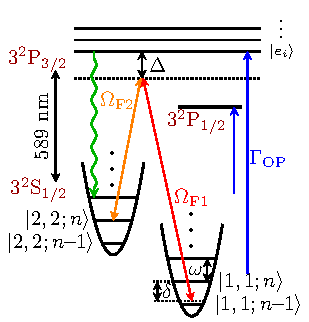
\includegraphics[width=8cm]{figures/na_rsc_schematics.pdf}
  \caption[Schematics of Raman sideband cooling for Sodium.]{
    Single Na atom Raman sideband cooling scheme.
    The Raman transitions couples $|2,2;n\rangle$ and $|1,1;n+\Delta n\rangle$
    through the intermediate states $|e_i\rangle$ in the $3^2P_{3/2}$ electronic states.
    The transitions have a one-photon detuning $\Delta_i\approx75$ GHz.
    Two-photon detuning, $\delta$, is defined relative to the $\Delta n=0$ carrier transition.
    For optical pumping, we use two $\sigma^+$ polarized transitions,
    one to pump the atom state out of $|1,1\rangle$ via $3^2P_{3/2}$
    and one to pump atoms out of $|2,1\rangle$ via $3^2P_{1/2}$
    to minimize heating of the $|2,2\rangle$ state.
    \label{fig:na-rsc-schematics}}
\end{figure}

The relevant energy diagram and the laser frequencies for RSC are shown in
Fig.~\ref{fig:na-rsc-schematics}.
We approximate the trapping potential using a harmonic oscillator.
Since this is a separable potential, we can use only the 1D motional state $|n\rangle$
and the result can be easily generalized to the full 3D system.

The cooling sequence consists of two types of pulses.
First, a Raman pulse drives the atom to a different hyperfine state while simultaneously
reduces the motional energy of the atom.
The optical pumping (OP) pulse afterwards then reset the hyperfine state of the atom
and reduce the entropy of the system.
This sequence is then repeated until the system reaches the ground motional state
where there is no more motional energy to be taken out of the system via the Raman pulse.
In this section, we will discuss the theory of each types of pulses individually.
We will cover how the pulses affect cooling performance in section \ref{ch:rsc-challenges}.

\subsection{Raman Transition}
\label{ch:rsc-basic-theory-raman}

As shown in Fig.~\ref{fig:na-rsc-schematics},
the cooling sequence starts with the sodium atom in the
$|s_1\rangle\equiv|2,2\rangle$ hyperfine state,
and a Raman transition is used to drive the atom to the $|s_2\rangle\equiv|1,1\rangle$ state,
where $|F,m_F\rangle$ denotes the $F$ and $m_F$ quantum number for the sodium atom.
The full Rabi frequency for such a transition is given by
\begin{align*}
  \Omega_R^0=&\sum_{i}\frac{\Omega_{1i}\Omega_{2i}^*}{2\Delta_i}
\end{align*}
where the sum is over all the coupled excited states,
$\Omega_{ai}\equiv\langle a|\mathbf{d}\cdot\mathbf{E}_a|e_i\rangle$ is the single photon
Rabi frequency between $|a\rangle$ and $|e_i\rangle$
and $\Delta_i$ is the single photon detuning from excited state $|e_i\rangle$.

In order to account for the motional degrees of freedom, we need to include the spatial
wavefunction of the atom and light into account.
As mentioned above, we approximate the atomic motional wavefunction by the harmonic oscillator
eigenstates $|n\rangle$. Coupling between states different $n$ states from the Raman transition
is allowed due to the recoil from the Raman lasers,
which corresponds to a spacial phase imprinting of $\ue^{\ui\mathbf{\Delta k}\cdot\mathbf{\hat x}}$
where $\mathbf{\Delta k}$ is the wavevector difference between the two Raman beams.
Using the creation ($\hat a^\dagger$) and annihilation ($\hat a$) operators and the relation
$\mathbf{\hat x}=\mathbf{x}_0\paren{\hat a+\hat a^\dagger}$ where $x_0=\sqrt{\hbar/2m\omega}$
is the harmonic oscillator length, the phase factor can be expressed as
$\ue^{\ui\eta^R\paren{\hat a+\hat a^\dagger}}$ where $\eta^R\equiv\mathbf{\Delta k}\cdot\mathbf{x}_0$
is the Lamb-Dicke parameter for the Raman transition \todo{\cite{}}.
The matrix element between motional state $|n\rangle$ and $|n'\rangle$ is therefore,
\[ M_{n,n'}=\langle n|\ue^{\ui\eta^R\paren{\hat a+\hat a^\dagger}}|n'\rangle \]
and the final Raman Rabi frequency between motional states $n$ and $n'$ is given by,
\[ \Omega_{R}^{n,n'}=M_{n,n'}\Omega_R^0 \]
For $n=n'$, this is called a carrier transition and the others are called sideband transitions.
If the final state is higher than the initial one, i.e. $n'>n$, it is a heating sideband.
Likewise, transitions with $n'<n$ are cooling sidebands.

A closed form result for $M_{n,n'}$ is given in \todo{\cite{}},
\[ M_{n,n'}=\ue^{\paren{\eta^R}^2/2}\sqrt{\frac{n_<!}{n_>!}}\paren{\eta^R}^{|n-n'|}L_{n_<}^{|n-n'|}\paren{\paren{\eta^R}^2} \]
where $n_<$ and $n_>$ are the lesser and greater, respectively, of $n$ and $n'$,
and $L_n^\alpha$ is the generalized Laguerre polynomial,
\[ L_n^\alpha(x)\equiv\sum_{m=0}^n(-1)^m\begin{pmatrix}n+\alpha\\n-m\end{pmatrix}\frac{x^m}{m!} \]

An important limit is the so-called Lamb-Dicke (LD) regime defined by $\paren{\eta^R}^2(2n+1)\ll 1$.
In this case, we can approximate the phase factor in leading order of $\eta^R$,
\[ \ue^{\ui\eta^R\paren{\hat a+\hat a^\dagger}}\approx1+\ui\eta^R\paren{\hat a+\hat a^\dagger} \]
and the matrix element
\[ M_{n,n'}\approx\delta_{n,n'}+\ui\eta^R\sqrt{n+1}\delta_{n+1,n'}+\ui\eta^R\sqrt{n}\delta_{n,n'+1} \]
the three terms corresponds to the carrier ($n'=n$),
the first order heating sideband ($n'=n+1$)
and the first order cooling sideband ($n'=n-1$) with corresponding strength
$1$, $\eta^R\sqrt{n+1}$ and $\eta^R\sqrt{n}$.
We can clearly see from this approximation that the coupling to other motional state
is stronger for a larger $\eta^R$ and higher motional quantum number $n$.
We will discuss this effect outside the LD regime and its implication
on the cooling performance in more detail in section \ref{ch:rsc-challenges}.

\subsection{Optical Pumping}
\label{ch:rsc-basic-theory-op}

Driving the system on a cooling sideband with Raman transition can reduce the
motional energy of the atom. However, this is a fully coherent process that does
not reduce the system entropy and is not really ``cooling'' the system
or achieving better control on the quantum state of the system.
Instead, quantum state control is achieved in the RSC via the OP pulse.
The initial hyperfine state $|2,2\rangle$ is a stretched state so it is the
state the system naturally ends up in when $\sigma^+$ light is applied.
However, if this is done using scattering from a $F=2$ to $F'=3$ transition,
the OP beam will allow continuous photon cycle
between the $|2,2\rangle$ and the $|3',3\rangle$ causing unnecessary motional heating during OP.
Therefore, the OP must be done on a $F=2$ to $F'=2$ transition.
Unfortunately, for Na, the corresponding transition from $3^2S_{1/2}$ to $3^2P_{3/2}$
that is used for the MOT is not useable due to the small energy difference of
$60 \mathrm{MHz}$ (or $6$ line widths) between the $F'=2$ and $F'=3$ states
\cite{steck_sodium_nodate}.
Instead, we must use the sodium $\mathrm{D1}$ line, i.e. $3^2S_{1/2}$ to $3^2P_{1/2}$ transition,
which lacks a $F'=3$ excited state.
The $\mathrm{D1}$ light with $\sigma^+$ polarization is only used to pump atoms from
$F=2$ states (in particular $|2,1\rangle$ which is populated during the OP process).
Since the goal of the OP pulse is to clear the atom population in all states but $|2,2\rangle$,
the photon cycling is not a concern for $F=1$ states and the $\mathrm{D2}$ line
is used for OP of $F=1$ states instead.
This also allow us to reuse the MOT light source and simplifies our setup.

\section{Raman Sideband Thermometry}

\todo{\cite{?}}From the discussion in section \ref{ch:rsc-basic-theory-raman},
we see that the strength of the sideband transition depends on the initial motional state
as well as the Lamb-Dicke parameter $\eta^R$ of the atom.
This dependency allows us to infer the motional state of the atom
by measuring the sideband height, i.e. the so-called sideband thermometry.

In particular, for atom with temperature $T$,
the probability for the atom to be in motional state $|n\rangle$ is,
\[ p_n=\frac{\ue^{-n\hbar\omega/k_BT}}{1-\ue^{-\hbar\omega/k_BT}} \]
for a Raman pulse with full Rabi frequency $\Omega_R^0$ and time $t$,
the peak height for the first order heating (+) and cooling (-) sidebands,
\begin{align*}
  h_\pm=&\sum_{n=0}^\infty p_n\sin^2\paren{\frac{\Omega_R^0t}{2}M_{n,n\pm1}}
\end{align*}
note that $p_{n+1}=p_n\ue^{-\hbar\omega/k_BT}$, $M_{n,n'}=M_{n',n}$ and $M_{n,-1}=0$, we have
\begin{align*}
  h_-=&\sum_{n=0}^\infty p_n\sin^2\paren{\frac{\Omega_R^0t}{2}M_{n,n-1}}\\
  =&\ue^{-\hbar\omega/k_BT}\sum_{n=1}^\infty p_{n-1}\sin^2\paren{\frac{\Omega_R^0t}{2}M_{n-1,n}}\\
  =&\ue^{-\hbar\omega/k_BT}h_+
\end{align*}
Therefore, if we measure the ratio of the cooling and heating sideband heights
$\alpha\equiv h_-/h_+$, we can calculate the temperature of the atom with
$\ue^{-\hbar\omega/k_BT}=\alpha$.
The corresponding ground state probability is,
\begin{align*}
  p_0=&\frac{1}{1-\ue^{-\hbar\omega/k_BT}}\\
  =&\frac{1}{1-\alpha}
\end{align*}
We will use this to experimentally characterize the performance of the cooling sequence
in the following sections.

\section{Setup}

\begin{figure}
  \centering
  \includegraphics[width=8cm]{figures/na_rsc_geometry.pdf}
  \caption[Beams and field geometry for Sodium Raman sideband cooling]{
    Geometry and polarizations of the Raman and optical pumping beams relative to the
    optical tweezer and bias magnetic field.
    Raman beams R1 and R4 address the radial $x$-mode.
    R1 and R2 address the radial $y$-mode.
    R3 and R4 address the axial $z$-mode, where the beams also couple to radial motion,
    but this coupling can be neglected when the atoms is cooled to the ground state of motion.
    \label{fig:na-rsc-geometry}}
\end{figure}

The geometry of all the beams and field involved is shown in Fig.~\ref{fig:na-rsc-geometry}.
In order to make the cooling more efficient and simplify the sideband thermometry,
we address the motion along the three principle axis of the tweezer using different pairs
of Raman beams.
We apply an external bias magnetic field of $8.8 \mathrm{G}$ parallel to the polarization
of the tweezer beam (and orthogonal to the tweezer beam propagation direction).
This makes the field orthogonal to the effective magnetic field of the tweezer,
which minimizes the vector light shifts~\cite{kaufman_cooling_2012,thompson_coherence_2013}.
Since the optical pumping beam requires $\sigma^+$ polarization,
it is setup to propagate parallel to the applied magnetic field.

\section{Cooling Performance and Challenge with Large Lamb-Dicke Parameter}
\label{ch:rsc-challenges}

\todo{some might belong to introduction of the chapter}
RSC is typically performed in the LD regime where the coupling
to other motional state is small.
Due to the light mass, short wavelength, limitted trap depth and high initial temperature
of the sodium atom however, we have to start our RSC sequence outside the LD regime.
This creates unique challenges to our experiment.
A detailed understanding of the cooling performance is required to understand
and overcome these challenges.

The simplest way to estimate the effectiveness of RSC
is by keeping track of the average energy of the atom during the cooling sequence.
For a typical RSC sequence in the LD regime, all the cooling are done on
the strongest first order cooling sideband.
The energy removed for atom driven in one Raman pulse is therefore, $\Delta E_-=\omega$.
In order to reinitialize the hyperfine state, the sodium atom needs to scatter on average
$2$ photons from the OP pulse which increases the average energy of the driven atom
by $\Delta E_+=4\omega_r$
\footnote{The factor of 4 comes from 2 absorbed photons and 2 reemitted photons.}
where $\omega_r\equiv \hbar k^2/2m$ is the recoil energy\cite{steck_sodium_nodate}
and $k$ is the OP light wave vector.
The heating to cooling ratio in one RSC pulse cycle is therefore,
\begin{align*}
  \frac{\Delta E_+}{\Delta E_-}=&\frac{2\hbar k^2}{m\omega}=4k^2x_0^2\\
  =&4\paren{\eta^{OP}}^2
\end{align*}
where $\eta^{OP}\equiv kx_0$ is the Lamb-Dicke parameter for OP.
Therefore, in order to achieve net cooling, we need $\paren{\eta^{OP}}^2<0.25$.
In 3D with cooling along multiple axis with different trapping frequency
(and therefore different $\eta^{OP}$), the $\paren{\eta^{OP}}^2$ in the requirement
is replaced by a weighted average of different axis depending on the frequency
each axis is cooled in the sequence.

\todo{change r to x in the plot to be consistent with text}
\begin{figure}
  \centering
  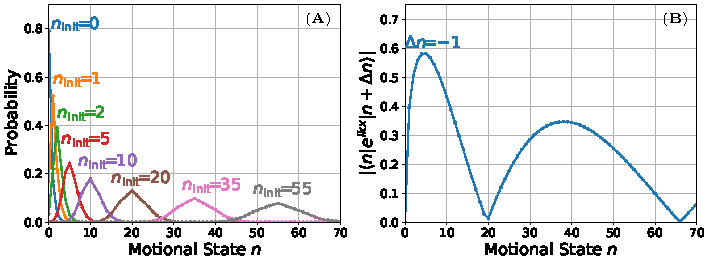
\includegraphics[width=\textwidth]{figures/na_rsc_challenges.pdf}
  \caption[Optical pumping motional-state redistribution and Raman coupling]{
    Optical pumping motional-state redistribution and Raman coupling for large LD parameters
    for the axial direction ($z$).
    The range plotted covers $95$\% of the initial thermal distribution.
    (A) Motional state distribution after one OP cycle for different initial states motion,
    $n_{\textrm{init}}$.
    Due to photon-recoil and the large LD parameter, $\eta^{\textrm{OP}}_z=0.55$,
    there is a high probability of $n$ changing.
    (B) Matrix elements for Raman transition on the first order cooling sideband
    deviate from $\sqrt{n}$ scaling with multiple minima.
    \label{fig:na-rsc-challenges}}
\end{figure}

In our experiment, the OP Lamb-Dicke parameters are
$\eta^{OP}_x, \eta^{OP}_y, \eta^{OP}_z = 0.25, 0.25, 0.55$.
Based on the metric above, any cooling sequences
that have fewer than $78\%$ cooling pulse for $z$ (axial) axis, which is generally the case,
should have a net cooling effect.
This, however, does not guarantee cooling into the ground motional state,
nor does it fully characterize the efficiency of the cooling sequence
since the averaging hides a few critical aspect of having a large Lamb-Dicke parameter.

One of the important effects can be seen in Fig.~\ref{fig:na-rsc-challenges}A showing
the motional state distribution after one OP cycle
for different initial motional states $n_{init}$.
Although the average heating is fixed at $4\omega_r$, independent of $n_{init}$,
the spread or the uncertainty of $n$ after the OP is significantly higher for high $n_{init}$.
This effect significantly increases the difficulty in controlling the state during the
RSC sequence. It can negatively impact the cooling performance and
may lead to increased loss during cooling due to atom escaping to higher motional states.

The other important effect is the dependency of matrix element $M_{n,n+1}$
on the motional level $n$.
While this dependency is not a new effect, since the $\sqrt{n}$ dependency
on the cooling sideband strength exist even in the LD regime
and must be taken into account with pulse time variation\todo{\cite{}}
to achieve efficient cooling, the high Lamb-Dicke parameter adds even more complications.
As shown in Fig.~\ref{fig:na-rsc-challenges}B, rather than a simple $\sqrt{n}$ dependency,
it is a non-monotonic function and more importantly has multiple minima, so-called ``dead-zone'',
within the range of motional states we are interested in.
The coupling strength for states in the dead-zones can be reduced by more than ten times
which can significant affect the efficiency of the cooling pulse
and even makes it virtually impossible to drive Raman transitions on atoms in these states
in order to cool them further.
A cooling sequence can therefore accumulate pupolations in the dead-zones
rather than the ground state.
Their small coupling strength also reduce their signal level during
Raman sideband spectroscopy making these states nearly invisible to sideband thermometry
which further complicates the optimization of the cooling sequence.

\section{Solution: High Order Sidebands}

\todo{change r to x in the plot to be consistent with text}
\begin{figure}
  \centering
  \includegraphics[width=8cm]{figures/na_rsc_mele_raman.pdf}
  \caption[Raman coupling including high order sidebands]{
    Matrix elements for Raman transition including high order sidebands.
    During cooling, we utilize the fact that high motional states couple most effectively
    to sidebands with large $|\Delta n|$ in order to overcome the issue with
    variation and dead zone in the coupling strengths.
    \label{fig:na-rsc-mele-raman}}
\end{figure}

The main solution to the issues related to the large Lamb-Dicke parameter
is in fact the large Lamb-Dicke parameter itself.
The increased coupling to other motional state for large Lamb-Dicke parameter
and high motional states applies not only to $|\Delta n|=1$ but to higher $\Delta n$ as well.
Fig.~\ref{fig:na-rsc-mele-raman} shows the coupling to higher order cooling sidebands
which all have comparable strengths as the first order sidebands in different ranges
of motional states.

Because of this, it is now possible, and in some cases preferred, to apply Raman cooling pulse
on the higher order sidebands instead of only the first order one.
These pulses reduce more energy from the system per pulse which directly improves
the cooling to heating ratio and allows better control on the motional state
given the uncertainty after an OP pulse.
More importantly, depending on the motional level, there is always a sideband order
with significant coupling strength that can be used to cool it,
therefore completely removing the coupling dead-zones.
Moreover, by using each sideband orders only near their coupling maxima,
the coupling strength variation is also greatly reduced which removes
the need to vary the pulse times for all but the pulses on the first order sideband.

\section{Solution: Simulation Based Optimization}

\ref{fig:na-rsc-sequence}

\begin{figure}
  \centering
  \includegraphics[width=\textwidth]{figures/na_rsc_sequence.pdf}
  \caption[Simulation optimized Raman sideband cooling sequence for Sodium]{
    Schematic of the cooling pulse sequence. The tweezer is strobed at 3 MHz to
    reduce light shifts during optical pumping~\cite{hutzler_eliminating_2017}.
    Each cooling cycle consists of $8$ sideband pulses.
    The four axial pulses address two sideband orders.
    The two pulses in each radial direction either address $\Delta n=-2$ and $\Delta n=-1$
    or have different durations to drive $\Delta n=-1$,
    at the end of the cooling sequence when most of the population is below $n=3$.
    The Raman cooling and spectroscopy pulses have Blackman envelopes~\cite{kasevich_laser_1992}
    to reduce off-resonant coupling,
    while the measurement Rabi pulses in Fig.~\ref{fig:na-rsc-rabi-flop}
    have square envelopes to simplify analysis.
    \label{fig:na-rsc-sequence}}
\end{figure}

\section{Calibration}
(Sideband/carrier)\todo{Use scattering to calibrate intensity}
(Cold vs hot)

\section{Cooling Performance}

\ref{fig:na-rsc-spectrum}
\ref{fig:na-rsc-rabi-flop}

\begin{figure}
  \centering
  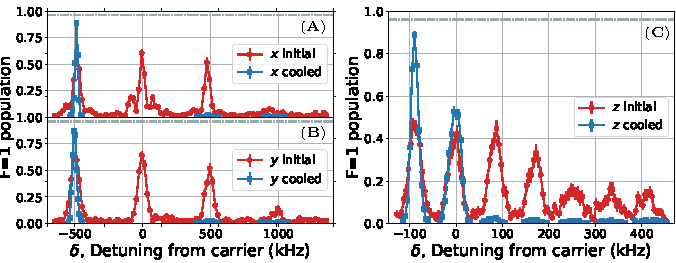
\includegraphics[width=\textwidth]{figures/na_rsc_spectrum.pdf}
  \caption[Raman sideband spectra before and after cooling]{
    Raman sideband spectra for (A) $x$, (B) $y$, (C) $z$ axis before (red circle)
    and after (blue square) applying Raman sideband cooling sequence.
    The height of the cooling sidebands (positive detuning)
    are strongly suppressed after cooling which suggests most of the atoms are cooled
    to the motional ground state in the trap.
    \label{fig:na-rsc-spectrum}}
\end{figure}

\begin{FPfigure}
  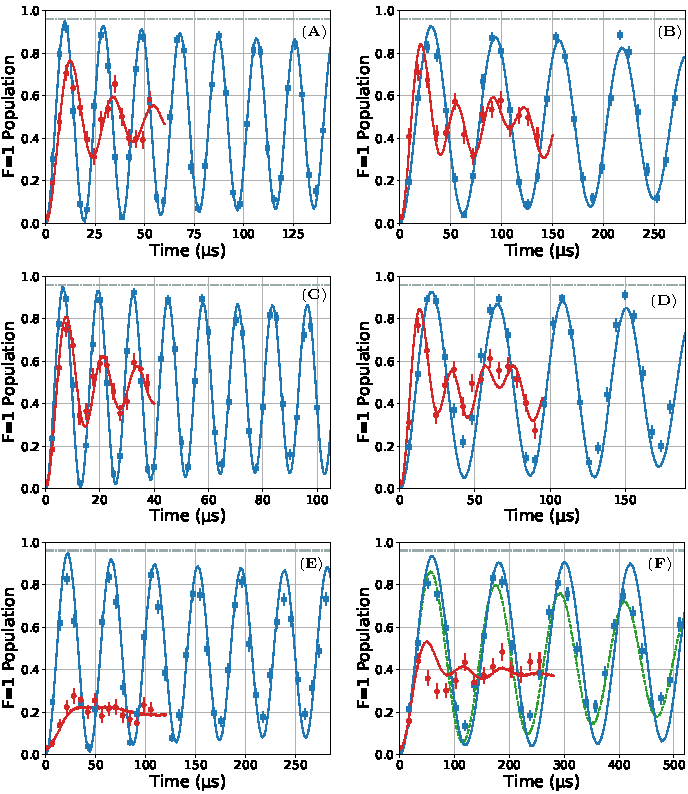
\includegraphics[width=\textwidth]{figures/na_rsc_rabi_flop.pdf}
  \caption[Rabi flopping on carriers and sidebands]{
    Rabi flopping on radial axis $x$ (A) carrier and (B) $\Delta n_x=1$ sideband,
    radial axis $y$ (C) carrier and (D) $\Delta n_x=1$ sideband,
    axial axis $z$ (E) carrier and (F) $\Delta n_x=1$ sideband,
    before (red circle) and after (blue square) Raman sideband cooling.

    Solid lines (both red and blue) in all plots are fits to a Rabi-flopping
    that includes a thermal distribution of motional states~\cite{meekhof_generation_1996}
    as well as off-resonant scattering from the Raman beams.

    The blue lines correspond to a ground state probability of (A-D) $98.1$\% along radial axis
    and (E-F) $95$\% along the axial axis after cooling.
    The red lines correspond to a thermal distribution of $80$ $\mu$K before RSC.
    The horizontal dashed lines in all the plots correspond to the $4\,\%$ probability
    of imaging loss.

    The green dashed line in (F) includes the additional decoherence due to
    a fluctuation of the hyperfine splitting of magnitude $3$ kHz.
    We see that the decoherence effect is strongest for the post-cooling data on
    the axial $\Delta n_z=1$ sideband where the Rabi frequency is the lowest.
    \label{fig:na-rsc-rabi-flop}}
\end{FPfigure}
\afterpage{\clearpage}

% Interaction of single atoms
% -*- mode: latex; TeX-engine: xetex; LaTeX-command-style: (("" "SOURCE_DATE_EPOCH=0 %(PDF)%(latex) --shell-escape %S%(PDFout)")); TeX-master: "../dissertation.tex"; -*-

\chapter{Interaction of Single Atoms}
\label{ch:interaction-shift}

\section{Introduction}
\label{ch:interaction-shift:introduction}

The interaction between the atoms is governed by the short range molecular potential.
For low energy processes with long de Broglie wavelength, however,
the complexity in the interaction at short range
can be ignored and the collision is approximately described by a single number,
the $s$-wave scattering length $a$.
Measuring the scattering length between the atoms allows us to probe the properties
of the molecular potential and refine our prediction on molecule formation,
e.g. the binding energy, without direct observation of the molecular states.
Traditionally, such measurements are done either by scattering in bulk gases
or by spectroscopy in optical lattices, both of which require the preparation
of many atoms in quantum degeneracy.
The preparation of two single atoms in the motional ground state in a single tweezer,
however, allow us to cleanly perform this measurement using only two atoms
and not affected by any many-body effects that inevitably exist using the traditional approach.

In this chapter, we will discuss our measurement of the interspecies scattering lengths
between multiple Na and Cs spin states using interaction shift spectroscopy.
We will start in section~\ref{ch:interaction-shift:theory}
with a theoretical description of two interacting atoms in an optical tweezer.
The experimental techniques and the result of the measurement will be described
in section~\ref{ch:interaction-shift:spectroscopy}.
The discussion here is based on our publication in~\cite{hood_multichannel_2020}.

\section{Two Interacting Atoms in Optical Tweezer}
\label{ch:interaction-shift:theory}

The Hamiltonian for two atoms in an harmonic potential with interaction is,
\[
  H=\sum_{i=x,y,z}\paren{\frac{m_{1}\omega_{1,i}^2r_{1,i}^2}{2}+\frac{p_{1,i}^2}{2m_{1}}}+\sum_{i=x,y,z}\paren{\frac{m_{2}\omega_{2,i}^2r_{2,i}^2}{2}+\frac{p_{2,i}^2}{2m_{2}}}+V_{\mathrm{int}}\paren{\mathbf{r}_1-\mathbf{r}_2}\numberthis{eq:interaction-shift:orig-hamiltonian}
\]
where $m_j$ is the mass of the $j$-th atom,
$r_{j,i}$, $p_{j,i}$, $\omega_{j,i}$ are the coordinate, momentum and trapping frequency
for the $j$-th atom along the $i$-th axis.
$V_{\mathrm{int}}$ is the interaction potential between the two atoms which is only a function
of the relative coordinate between the atoms $\mathbf{r}_1-\mathbf{r}_2$.

Since the two atoms experience the same trapping light field,
their trapping potential has the same center and the same shape.
However, due to the difference in the polarizability between the atoms,
the trap depth can be different.
Nevertheless, in our experiment, depending on the trapping wavelength,
we have $\omega_{1,i}\approx\omega_{2,i}$ to within $10~\mathrm{\%}$ to $20~\mathrm{\%}$
and this is the regime we will mainly focus on in this section.

In order to calculate the interaction term, we can change from the coordinates for
the two individual atoms to the center of mass~(COM) and relative coordinates.
\begin{align*}
  R_i=&\ \frac{m_1r_{1,i}+m_2r_{2,i}}{m_1+m_2}&r_{\mathrm{rel},i}=&\ r_{1,i}-r_{2,i}\\
  P_i=&\ p_{1,i}+p_{2,i}&p_{\mathrm{rel},i}=&\ \frac{m_2p_{1,i}-m_1p_{2,i}}{m_1+m_2}
\end{align*}
The corresponding masses and trapping frequencies are,
\begin{align*}
  M=&\ m_1+m_2&\mu=&\ \frac{m_1m_2}{m_1+m_2}\\
  \Omega_i^2=&\ \frac{m_1\omega_{1,i}^2+m_2\omega_{2,i}^2}{m_1+m_2}&\omega_{\mathrm{rel},i}^2=&\ \frac{m_2\omega_{1,i}^2+m_1\omega_{2,i}^2}{m_1+m_2}
\end{align*}
and the Hamiltonian can be expressed as,
\begin{align*}
  \begin{split}
    H=&\sum_{i=x,y,z}\paren{\frac{M\Omega_{i}^2R_{i}^2}{2}+\frac{P_{i}^2}{2M}}+
    \left[\sum_{i=x,y,z}\paren{\frac{\mu\omega_{\mathrm{rel},i}^2r_{\mathrm{rel},i}^2}{2}+\frac{p_{\mathrm{rel},i}^2}{2\mu}}+
      V_{\mathrm{int}}\paren{\mathbf{r}_{\mathrm{rel}}}\right]\\
    &+\sum_{i=x,y,z}\mu\paren{\omega_{1,i}^2 - \omega_{2,i}^2}R_ir_{\mathrm{rel},i}
  \end{split}\numberthis{eq:interaction-shift:full-hamiltonian}
\end{align*}
The first term and the second term only relies on the COM motion and relative motion
respectively and can be solved independently. The third term mixes the COM and relative motion
and is proportional to the trapping frequency difference.
If the trapping frequencies are the same for the two atoms, the third term is $0$ and
the solution is fully separable.
As mentioned above, since the trapping frequencies for the two atoms are similar,
we will assume the mixing term is small and treat it as a small correction in the calculation.

The interaction potential $V_{\mathrm{int}}$ is the original for
the molecular bound states and its exact form will be discussed in chapter~\ref{ch:pa},
\ref{ch:raman-spectroscopy} and \ref{ch:raman-transfer}.
However, since the range of the potential is much smaller than
the size of the atomic wavefunction, we can ignore the short range details of the potential
and treat it as a contact interaction characterized only by
the scattering length $a$~\cite{busch_two_1998},
\[
  V_{\mathrm{int}}\paren{\mathbf{r}}=\frac{2\pi\hbar^2a}{\mu}\delta_{\mathrm{reg}}\paren{\mathbf{r}}
\]
where $\mu = m_1m_2/\paren{m_1+m_2}$ is the reduced mass and
$\delta_{\mathrm{reg}}\paren{\mathbf{r}}\equiv\delta^{(3)}\paren{\mathbf{r}}\paren{\partial/\partial r}r$
is the regularized delta-function.
The validity of the pseudo-potential is characterized by the ratio of
the van der Waals length $\beta_6 = (2\mu C_6 / \hbar^2)^{1/4}$
to the relative harmonic oscillator lengths $\beta_{\mathrm{rel},i}$~\cite{
  bolda_effective-scattering-length_2002,blume_fermi_2002}.
In our experiment, these are $\beta_6 \approx 6~\mathrm{nm}$,
$\beta_{\mathrm{rel},x} \approx \beta_{\mathrm{rel},x}\approx 66~\mathrm{nm}$ for the radial axes,
and  $\beta_{\mathrm{rel},z} \approx 158~\mathrm{nm}$ for the axial axis.

\subsection{Perturbative Calculation}
\label{ch:interaction-shift:theory:perturb}

For weak interaction, i.e. a small scattering length $a$, the effect of the interaction
on the energy level can be calculated perturbatively.
The result from this calculation is useful for checking the validity of the full calculation,
as well as providing an intuitive understanding of the shift and its dependency
on different parameters.

For simplicity, we will assume all the trapping frequencies are the same,
i.e. $\omega_{1,i}=\omega_{2,i}=\omega_{\mathrm{rel},i}=\Omega_i=\omega_i$,
so that we only need to consider the relative motion,
\[
  H_{\mathrm{rel}}=\sum_{i=x,y,z}\paren{\frac{\mu\omega_{i}^2r_{\mathrm{rel},i}^2}{2}+\frac{p_{\mathrm{rel},i}^2}{2\mu}}+
  V_{\mathrm{int}}\paren{\mathbf{r}_{\mathrm{rel}}}
\]
When treating the interaction as perturbation, the base solution is the harmonic oscillator
states for the relative motion $|n_{\mathrm{rel},x},n_{\mathrm{rel},y},n_{\mathrm{rel},z}\rangle$.
The energy level perturbation is then,
\begin{align*}
  \Delta_{n_{\mathrm{rel},x},n_{\mathrm{rel},y},n_{\mathrm{rel},z}}=&\langle n_{\mathrm{rel},x},n_{\mathrm{rel},y},n_{\mathrm{rel},z}|V_{\mathrm{int}}\paren{\mathbf{r}_{\mathrm{rel}}}|n_{\mathrm{rel},x},n_{\mathrm{rel},y},n_{\mathrm{rel},z}\rangle\\
  =&\frac{2\pi\hbar^2a}{\mu}\langle n_{\mathrm{rel},x},n_{\mathrm{rel},y},n_{\mathrm{rel},z}|\delta_{reg}\paren{\mathbf{r}_{\mathrm{rel}}}|n_{\mathrm{rel},x},n_{\mathrm{rel},y},n_{\mathrm{rel},z}\rangle\\
  =&\frac{2\pi\hbar^2a}{\mu}\abs{\psi_{n_{\mathrm{rel},x},n_{\mathrm{rel},y},n_{\mathrm{rel},z}}(0)}^2\numberthis{eq:interaction-shift-perturb-shift}
\end{align*}
where $\abs{\psi_{n_{\mathrm{rel},x},n_{\mathrm{rel},y},n_{\mathrm{rel},z}}(0)}^2$ is the probability density
for zero distance between the atoms.

For the motional ground state, the shift is,
\begin{align*}
  \Delta_{0,0,0}=&a\frac{2\hbar^2}{\mu\sqrt{\pi}}\prod_{i=x,y,z}\frac{1}{\beta_{\mathrm{rel},i}}
\end{align*}
where $\beta_{\mathrm{rel},i}\equiv\sqrt{\hbar/\mu\omega_{\mathrm{rel},i}}$ is the relative motion
oscillator length along the $i$-th axis.
The shift is proportional to the strength of the interaction $a$,
and is also stronger for stronger confinement where the wavefunction density is higher.

We can see from Eq.~\ref{eq:interaction-shift-perturb-shift} that the shift is only
non-zero when all of $n_{\mathrm{rel},i}$'s are even.
The shift is also smaller for higher motional excited state with smaller wavefunction density.
This means that the shift will only be observable if the atom is cooled to close to
the motional ground state and will be small or zero for hot atoms.

\subsection{Non-perturbative Calculation}
\label{ch:interaction-shift:theory:non-perturb}

The first order perturbative result breaks down for large $a$ when the energy shift
approaches the motional energy scale $\omega_{\mathrm{rel},i}$.
Moreover, due to the divergent nature of the delta-function in the contact interaction potential,
higher order perturbative calculation does not converge.
It is therefore necessary to use a non-perturbative solution of the interacting atoms
in order to interpret measurements of the shift for strong interaction.
To do this, we first ignore the last term in
the Hamiltonian~\ref{eq:interaction-shift:full-hamiltonian} so that it is fully separable
into COM and relative motion.

For the relative Hamiltonian, we use the analytic cylindrical solutions
from Ref.~\cite{idziaszek_analytical_2006}.
These solutions require the potential to be cylindrically symmetric and
that the ratio between the radial trapping frequency
and the axial trapping frequency $\eta\equiv\omega_{\mathrm{radial}}/\omega_z$
to be an integer.
We therefore define $\eta = 6$, which is close to the actual values of $5.6$
and ignores the $7~\mathrm{\%}$ difference between the two radial trapping frequencies
in order to use these solutions.
These differences from the real Hamiltonian will be included later,
together with the mixing term, as a correction~\cite{
  bertelsen_association_2007,deuretzbacher_heteronuclear_2008}.
The analytic solutions are only given for the interacting states,
but there are also many relative states which have zero wavefunction at the $\delta$-function,
and therefore are unaffected.
We have identified these states from the perturbative calculation
in section~\ref{ch:interaction-shift:theory:perturb}
which are states with $l\ne0$ or odd $m_z$
after transforming to the cylindrical coordinate used by the analytic solution,
where $l$ is the angular momentum quantum numbers for the radial part,
and $m_z$ is quantum number for 1D harmonic oscillator for the axial part.
The complete basis includes both the interacting states from
Ref.~\cite{idziaszek_analytical_2006} as well as all of the non-interacting states.
The non-interacting states are solutions to the cylindrical harmonic oscillator,
and so are just cylindrical harmonic oscillator wavefunctions with eigenenergies
\begin{align*}
  \frac{E_{n,l,m_z}}{\hbar\omega_z}=&\paren{2 n + |l| + 1}\eta + \paren{m_z + 1/2}
                                      \numberthis{eq:interaction-shift:cylind-E}
\end{align*}
where $n$ is the principal quantum number for the radial part.
In order to find the non-interacting wavefunction,
we need to remove the interaction wavefunction from
the cylindrical harmonic oscillator wavefunctions.
The complication in this process is that when $\eta$ is an integer,
as is required by the solution of the interaction,
there is a subspace of cylindrical harmonic oscillator states with $l=0$
and even $m_z$ that are degenerate from Eq.~\ref{eq:interaction-shift:cylind-E}.
In each degenerate subspace with $N_{\mathrm{deg}}$ states,
the non-interacting states $\psi_{\mathrm{non-int}}$
are a linear superposition of the degenerate eigenstates $\psi_i$
that satisfies the condition $V_{\mathrm{int}}\psi_{\mathrm{non-int}} = 0$ or
$\psi_{\mathrm{non-int}}\paren{\mathbf{r}_{\mathrm{rel}}=0}=0$.
We find these amplitudes $c_i$ using a Gram-Schmidt procedure,
which from the requirement $\sum_{i=1}^{N_{\mathrm{deg}}}  c_i \psi_i\paren{\mathbf{r}_{\mathrm{rel}}=0} = 0$.
In each subspace, there is only one interacting state,
for which the analytic solution is used, and  $N_{\mathrm{deg}}-1$ non-interacting states.

For the interacting states,
the energies are given by the transcendental equations~\cite{idziaszek_analytical_2006}
\begin{align*}
  \mathcal{F}\paren{-\frac{\paren{E-E_0}}{2}, \eta}=&-\frac{\sqrt{2\pi}}{a}
\end{align*}
where $\mathcal{F}\paren{x, \eta}$ is given by
\begin{align*}
  \mathcal{F}\paren{x, \eta}=
  &\frac{\sqrt{\pi} \Gamma(x)}{\Gamma(x+\frac{1}{2})}
    \sum_{m=1}^{n-1} F\paren{1,x;x+\frac{1}{2} ; e^{\ui(2\pi m/ \eta)}}
    -\frac{2 \sqrt{\pi} \Gamma(x)}{\Gamma(x-\frac{1}{2})}
\end{align*}
Here $F(a,b;c,x)$ denotes the hypergeometric function
and $\Gamma(x)$ is the Euler gamma function.
The energy $E$ and $E_0$ are in units of the axial trapping frequency $\omega_z$,
and so the ground state energy $E_0 = \eta + 1/2$.

The COM Hamiltonian is a cylindrical harmonic oscillator and the energy is given by
Eq.~\ref{eq:interaction-shift:cylind-E}.

\begin{figure}
  \centering
  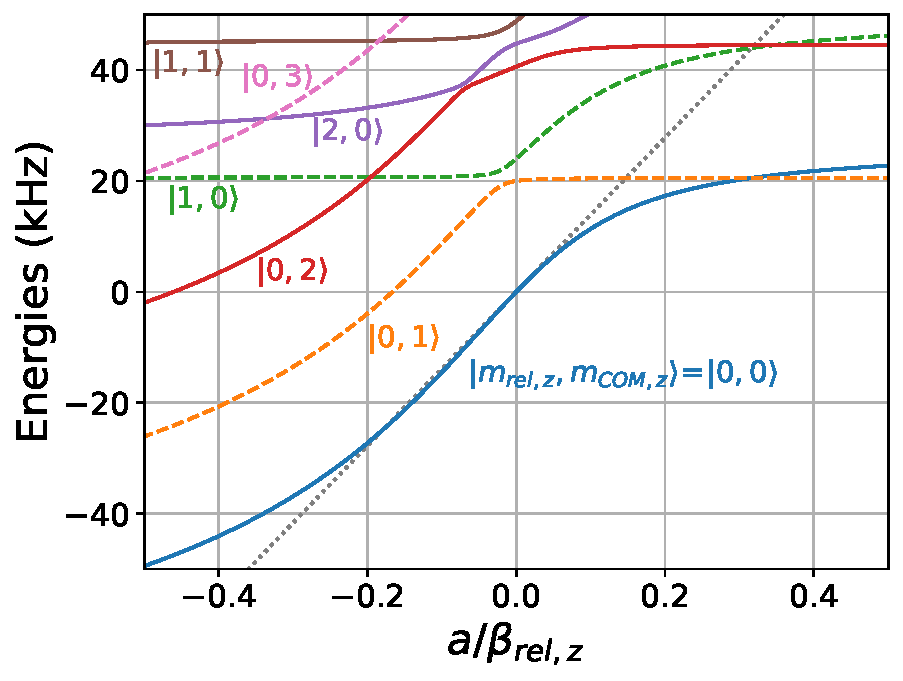
\includegraphics[width=0.7\textwidth]{figures/interaction_shift_energies.pdf}
  \caption[Result of interaction shift calculation.]{
    Energy levels as a function of scattering length
    (in unit of the axial relative motion oscillator length
    $\beta_{\mathrm{rel},z}$) from the non-perturbative calculation.
    The dashed straight light is the result from first order perturbation
    for the motional ground state which shows good agreement with the exact calculation
    at small scattering length.
    Only states that are in the radial motional (both relative and COM) ground state
    are shown because of the high radial motional energy scale~($100~\mathrm{kHz}$).
    The states are labeled with their relative and COM axial motional quantum numbers
    $m_{\mathrm{rel},z}$ and $m_{\mathrm{COM},z}$.
    Due to the relative and COM motion mixing term and the resulting avoided crossings
    in the energy levels, these are not the true quantum numbers
    and are not constants along the same line.
    The numbers shown in the plot are for the state at large negative scattering length.
    States with even total parity, i.e. $m_{\mathrm{rel},z} + m_{\mathrm{COM},z}$, are plotted in solid lines
    whereas ones with odd total parity are plotted in dashed lines.
    Since the Hamiltonian conserves total parity,
    there is no coupling between the two sets of states
    which results in the level crossing shown in the plot.
    \label{fig:interaction-shift:energies}}
\end{figure}

Now that we have the solution in the separable and cylindrical case,
the next step is to include the non-separable and asymmetric correction terms
by diagonalizing the total matrix in the combined COM and relative cylindrical bases.
Compared to treating the interaction term in Eq.~\ref{eq:interaction-shift:orig-hamiltonian}
as a perturbation, the correction terms included here all have the form of
harmonic potentials and therefore have much better convergence behavior.
We include all states with energies up to $20 \omega_{\mathrm{rel},z}$ in the calculation.
The matrix elements are calculated numerically using the cylindrical wavefunctions,
which for completeness are given here:
\begin{align*}
  \Psi_{n,l,m_z}\paren{\rho,\theta,z}=
  &\Psi^{\mathrm{radial}}_{n,l}\paren{\rho, \theta}\Psi^{\mathrm{axial}}_{m_z}\paren{z}
\end{align*}
with the normalized radial harmonic oscillator wavefunction,
\begin{align*}
  \Psi^{\mathrm{radial}}_{n,l}\paren{\rho, \theta}=
  &\sqrt{\frac{2n!}{a_\perp^2 (n+|l|)!}} e^{-r^2/(2 a_\perp^2)} \paren{\frac{r}{a_\perp}}^{|l|}
    L_n^{|l|}\paren{\frac{r^2}{a_\perp^2}} \frac{ e^{i l \theta}}{\sqrt{2 \pi}}
\end{align*}
and the normalized 1D harmonic wavefunction,
\begin{align*}
  \Psi^{\mathrm{axial}}_{m_z}(z)=&\frac{1}{\sqrt{2^{m_z} m_z!}} \frac{1}{\sqrt{a_z}(\pi)^{1/4}}
                                   e^{-z^2/(2 a_z)} H_{m_z}(z/a_z)
\end{align*}
Here the radial and axial oscillator lengths are defined as
$a_\perp = \sqrt{\hbar/(\mu \omega_\perp)}$ and $a_z = \sqrt{\hbar/ (\mu \omega_z)}$.
$H_{m_z}$ are the Hermite-Gaussian functions,
and $L^{|l|}_n$ are the generalized Laguerre polynomials.

The eigenenergies of the matrix are calculated as a function of the scattering length.
The results for the lowest energy ones are shown in Fig.~\ref{fig:interaction-shift:energies}.

\section{Interaction Shift Spectroscopy}
\label{ch:interaction-shift:spectroscopy}

\subsection{Experiment Sequence}
\label{ch:interaction-shift:spectroscopy:sequence}
The absolute energies shown in Fig.~\ref{fig:interaction-shift:energies} have an arbitrary global
offset and are therefore not directly measurable.
Instead, the measurable quantities are the energy differences between different states,
which can be done either by changing the scattering length, i.e. moving along the x axis,
or by changing the motional state of the atoms, i.e. moving along the y axis.

\begin{figure}
  \centering
  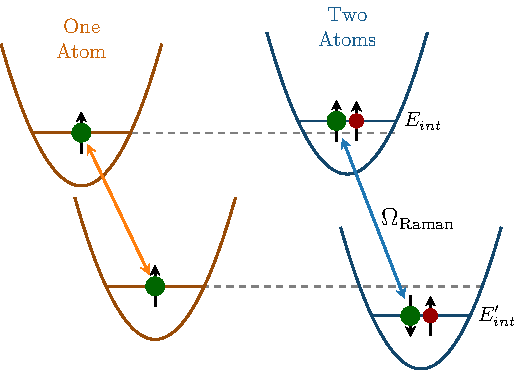
\includegraphics[width=0.7\textwidth]{figures/interaction_shift_measure.pdf}
  \caption[Schematics of interaction shift spectroscopy.]{
    Schematics of interaction shift spectroscopy using Raman transitions.
    Left: Raman resonance for atomic spin flip with only one atom in the tweezer.
    Right: The energy shifts by a spin state dependent amount with the present of
    the second~(red) atom. This causes a shift in the spin flip resonance frequency
    for the first~(green) atom compared to the one atom case.
    The shift corresponds to the difference in the interaction shift between the
    two spin states.
    \label{fig:interaction-shift:measure}}
\end{figure}

In our experiment, we measure the interaction shifts by flipping the spin state of
one but not the other atom using Raman transition.
Since the scattering length depends on the spin state,
this allows us to measure the difference between energy levels for different scattering lengths
by comparing the resonance frequency in the absence of
the other atom~(Fig.~\ref{fig:interaction-shift:measure}).
The spin flip is done in the same $8.8~\mathrm{G}$ we use for
Raman sideband cooling~(section~\ref{ch:rsc:setup}).
We drive the transition using two Raman beams that are co-propagating
which imprints no phase gradient on
the atomic wavefunction~(section~\ref{ch:rsc:basic-theory:raman}).
This reduces the number of observable resonances and provides a cleaner spectrum since,
\begin{enumerate}
\item Parity is conserved during the transition.\\
  Starting from the motional ground state, this means that all dashed lines in
  Fig.~\ref{fig:interaction-shift:energies} are uncoupled.
\item Coupling to different motional states are surppressed.\\
  In particular, this reduces the coupling to COM motional excitation
  in the strong interaction limit.
  Note that since the interaction between the atoms modifies the wavefunction,
  there is still non zero overlap between different motional states
  especially for the relative motion.
\end{enumerate}

\subsection{Results}
\label{ch:interaction-shift:spectroscopy:results}

\begin{figure}
  \centering
  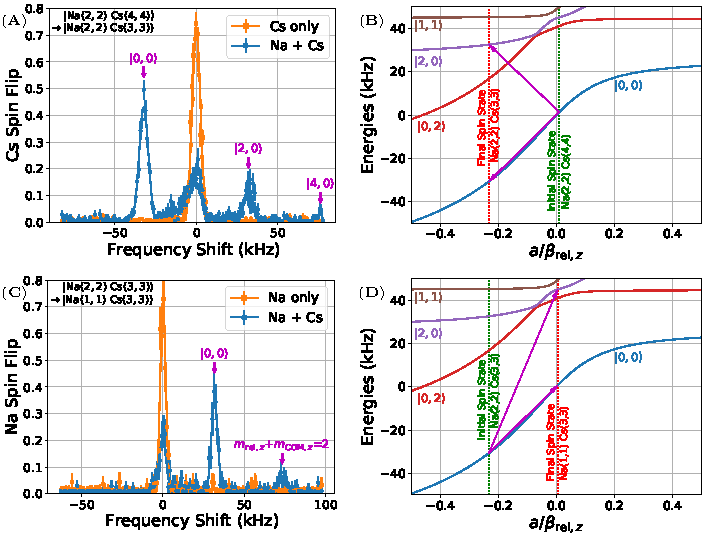
\includegraphics[width=\textwidth]{figures/interaction_shift_results.pdf}
  \caption[Interaction shift measurement results.]{
    Interaction shift measurement for
    (A) $|\mathrm{Na(2, 2),Cs(4, 4)}\rangle\rightarrow|\mathrm{Na(2, 2),Cs(3, 3)}\rangle$
    and (C) $|\mathrm{Na(2, 2),Cs(3, 3)}\rangle\rightarrow|\mathrm{Na(1, 1),Cs(3, 3)}\rangle$
    with the corresponding transition shown on the energy map from theoretical calculation
    in (B) and (D) respectively.
    The orange line shows the bare resonance with only one atom in the trap
    and the blue line shows the spectrum including interaction shift.
    A resonance appearing at positive frequency shift corresponds to the final state
    having a more positive energy (more repulsive interaction or higher motional energy).
    More than one shifted peaks can be observed due to the motional state mixing caused
    by the interaction. The corresponding motional state is marked as
    $|m_{\mathrm{rel},z},m_{\mathrm{COM},z}\rangle$ on the resonance.
    For the $|\mathrm{Na(2, 2),Cs(3, 3)}\rangle\rightarrow|\mathrm{Na(1, 1),Cs(3, 3)}\rangle$
    transition (C and D), the states with two quanta of total axial excitation are unresolved.
    Since the Raman transition preserves parity, only states with even parity are shown
    in (B) and (D).
    \label{fig:interaction-shift:results}}
\end{figure}

The spectrum for the $|\mathrm{Na(2, 2),Cs(4, 4)}\rangle$ to $|\mathrm{Na(2, 2),Cs(3, 3)}\rangle$
transition is shown in Fig.~\ref{fig:interaction-shift:results}A.
The orange line shows the bare $|\Cs(4, 4)\rangle$ to $|\Cs(3, 3)\rangle$ resonance without
the presence of the Na atom whereas the blue line shows the resonances
including the interaction with the Na atom.
The largest peak on the left is the shifted ground motional state
$|m_{\mathrm{rel},z},m_{\mathrm{COM},z}\rangle = |0,0\rangle$ and the smaller peak on the right
corresponds to the $|2,0\rangle$ state~(Fig.~\ref{fig:interaction-shift:results}B).
A even smaller resonance for $|4,0\rangle$ is also visible further right
(not shown in Fig.~\ref{fig:interaction-shift:results}B).
The $|0,0\rangle$ resonance gives the difference of the interaction shifts
of the initial and final spin states,
$E(\mathrm{Na(2, 2),Cs(3, 3)}) - E(\mathrm{Na(2, 2),Cs(4, 4)})=-32.1(2) \mathrm{kHz}$.
The peak near zero frequency corresponds to the initial Na and Cs population that is not prepared
in the motional ground state or an interacting state.
The fitted height $0.46$ of the $|0,0\rangle$ peak serves as a lower bound for
the relative motional ground-state population.
Similarly, Fig.~\ref{fig:interaction-shift:results}C shows the result for
the $|\mathrm{Na(2, 2),Cs(3, 3)}\rangle$ to $|\mathrm{Na(1, 1),Cs(3, 3)}\rangle$
measured by driving a Na Raman transition.
Two interaction shifted resonances were observed which corresponds to
the motional ground state and unresolved states with two total
Na and Cs motional excitation~(Fig.~\ref{fig:interaction-shift:results}D).

\begin{table}
  \centering
  \caption[Interaction shift and scattering lengths.]{
    Interaction shift and scattering lengths for different spin states.
    The number for the $|\mathrm{Na(2, 2),Cs(4, 4)}\rangle$ is computed from
    the binding energy of the molecular state whereas the other numbers are
    measured by the interaction spectroscopy.
    \label{table:interaction-shift:results}}
  \begin{tabular}{|c|c|c|}
    \hline
    Spin state&Interaction Shift (kHz)&Scattering Length\\\hline
    $|\mathrm{Na(2, 2),Cs(4, 4)}\rangle$&$1.40$&$30.4a_0$\\\hline
    $|\mathrm{Na(2, 2),Cs(3, 3)}\rangle$&$-30.7$&$-693.8a_0$\\\hline
    $|\mathrm{Na(1, 1),Cs(3, 3)}\rangle$&$0.62$&$13.7a_0$\\\hline
  \end{tabular}
\end{table}

Since the measurement only give the energy difference between different scattering lengths,
we determine an absolute interaction shift of the $|\mathrm{Na(2, 2),Cs(4, 4)}\rangle$
using the binding energy of
the least bound state $v''=-1$~(section~\ref{ch:raman-spectroscopy:states:n0}).
The absence of spin mixing for this state allows its binding energy to be related
to the scattering length directly through
the single-channel quantum defect theory~(QDT)~\cite{
  gao_quantum-defect_1998,gao_angular-momentum-insensitive_2001,gao_general_2008}
but extended to two-scale by including the $-C_8/r^8$ potential.
For the van der Waals coefficients, we use $C_6=3227~\mathrm{a.u.}$ and
$C_8=3.681\times10^5~\mathrm{a.u.}$ from
Refs.~\cite{docenko_coupling_2006,mcguyer_high-precision_2015,porsev_accurate_2003}.
From here, we can use the result of the calculation above to obtain all the
absolute interaction shifts and scattering lengths.
The final result for all the spin states is summarized in
table~\ref{table:interaction-shift:results}.

\section{Summary and Outlook}
\label{ch:interaction-shift:summary}
Optical tweezer provides a clean platform to study the interaction between exactly two atoms.
Here, we started our exploration of the interaction by measuring the most important quantity
for $s$-wave scattering process at ultracold temperature, the scattering length $a$.
The results from these measurements can be used
to refine the theoretical model of the NaCs molecule,
including predictions of the molecule binding energy
and Feshbach resonances~\cite{hood_multichannel_2020}.
More properties of the interaction will be studied in the following chapters.

Additionally, the combination of the tight confinement from the optical tweezer
and the interaction between the atoms also give us further control
on the motional states of the atom.
As we have seen in this chapter, the degeneracy of carrier Raman transition
for different motional states is lifted by the interaction.
As a result, driving on the $|0,0\rangle\rightarrow|0,0\rangle$ interaction shifted resonance
allows us to prepare a system that is completely in the ground state of the relative motion.
This will be used when we coherently create the molecules~(chapter~\ref{ch:raman-transfer})
to lower the requirement for the cooling and reduce the background caused by hot atoms.

% Photoassociation of single atoms
% -*- mode: latex-mode; TeX-engine: xetex; LaTeX-command-style: (("" "SOURCE_DATE_EPOCH=0 %(PDF)%(latex) --shell-escape %S%(PDFout)")); TeX-master: "../dissertation.tex"; -*-

\chapter{Photoassociation of Single Atoms}
\label{ch:pa}

\section{Introduction}

The method we use to coherently create a single molecule from atoms
uses two-photon optical transition~(chapter~\ref{ch:raman-transfer}).
Before we can drive such a transition, however, we must locate and characterize
the intermediate excited states of the molecule to be used in the two-photon transition.
This can be measured using photoassociation~(PA) spectroscopy
where two atoms are driven from the atomic state to an excited molecular state
via an optical transition.
The flexibility of the optical tweezer platform allows us to
prepare a clean initial state with only two atoms
as well as accurately detect when PA has happened
with high signal to noise ratio~(section~\ref{ch:pa:sequence-res}).

In this chapter, we describe the molecular energy structure~(section~\ref{ch:pa:structure})
and how we use PA spectruscopy to locate and
identify the molecular excited states~(section~\ref{ch:pa:pa}).
We also details the beampath for the measurement~(section~\ref{ch:pa:beampath}) including
the alignment procedure for the PA beam and discussions about factors that can affect
the PA linewidth~(section~\ref{ch:pa:linewidth}).

\section{Energy Levels}
\label{ch:pa:structure}

First we will discuss the energy levels in a diatomic molecule
as well as the labeling system for the states.
We will focus mainly on the electronic excited states measured in this chapter
but most of the discussion here applies to ground electronic states as well
and will be useful for chapter~\ref{ch:raman-spectroscopy} and \ref{ch:raman-transfer}.

\subsection{Angular Momentums}

Compared to an atom, a diatomic molecule has many more degrees of freedoms.
In additional to the quantum numbers for each atom in the molecule,
molecules also have nuclear motion.
In order to reduce the complexity, it is therefore very important to consider the
symmetry of the system, and in particular the angular momentums,
which corresponds to rotation symmetry, and the coupling between them.
The angular momentums in a diatomic molecule includes electron orbit $\mathbf{L}$
\footnote{There are $\mathbf{L}_1$ and $\mathbf{L}_2$ for the two electron but since
  we only consider states with at most one $\mathbf{L}_i\neq0$ we will only use one quantum number here},
electron spin $\mathbf{S}_1$ and $\mathbf{S}_2$, nuclear orbital $\mathbf{N}$
and nuclear spin $\mathbf{I}_1$ and $\mathbf{I}_2$.
Although the total angular momentum
$\mathbf{F}\equiv\mathbf{L}+\mathbf{S}_1+\mathbf{S}_2+\mathbf{N}+\mathbf{I}_1+\mathbf{I}_2$
is the only true conserved quantity in the absence of external field,
depending on the coupling strengths between the angular momentums,
there are additional approximately conserved quantity in the molecule.

For the NaCs molecule and our experiment, there are two important regimes where the coupling
strength can be easily ordered.

\subsubsection{Deeply Bound States}
\label{ch:pa:angular-momentums:deep}

\begin{figure}
  \centering
  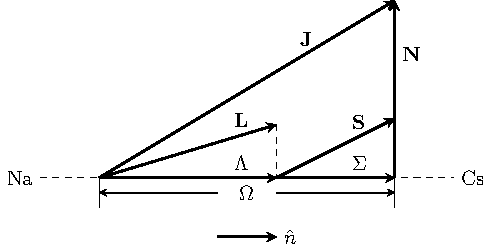
\includegraphics[width=\textwidth]{figures/pa_hunds_case_a.pdf}
  \caption[Hund's~case~(a)]{
    Angular momentum coupling for \textit{Hund's~case~(a)}.
    $\mathbf{L}$ and $\mathbf{S}$ are coupled to the internuclear axis $\hat n$
    and the sum of the projections $\Omega=\Lambda+\Sigma$ is then
    added with the orthogonal compoment $\mathbf{N}$ to form $\mathbf{J}$.
    \label{fig:pa:hunds-case-a}}
\end{figure}

This is described by the \textit{Hund's~case~(a)}~\cite[p.~523-626]{bransden_physics_2003}.
Molecular states with large binding energies mostly experience interactions
between the atoms at short range where the electric static interaction is very strong.
This couples the the two electron spins into a total electron spin
$\mathbf{S}\equiv\mathbf{S}_1+\mathbf{S}_2$ via a very strong effective interaction
of the form $\mathbf{S}_1\cdot\mathbf{S}_2$ which originates
from the resulting symmetry of the electron orbital wavefunction.
Similar to atoms, the nuclear spin interaction is also very week compared to
other energy scales so we can ignore the hyperfine structure and only need to consider
$\mathbf{J}\equiv\mathbf{L}+\mathbf{S}+\mathbf{N}$.

The strong electrostatic interaction also creates an effective coupling
between the $\mathbf{L}$ and $\mathbf{S}$ with the internuclear axis $\hat{n}$
causing $\mathbf{L}$ and $\mathbf{S}$ to process rapidly around $\hat{n}$.
This creates two new conserved quantity $\Lambda$ and $\Sigma$
as the projection of $\mathbf{L}$ and $\mathbf{S}$
along $\hat{n}$ respectively.
The total angular momentum along $\hat{n}$ is therefore $\Omega\equiv\Lambda+\Sigma$
and it is added to the $\mathbf{N}$ which is orthogonal to $\hat{n}$ to form
the total angular momentum $\mathbf{J}$~(Fig.~\ref{fig:pa:hunds-case-a}).

The angular momenum state of the molecule is therefore fully characterized by
$|L,\Lambda,S,\Omega,J\rangle$. $\Lambda$ can be $0,1,\dots,L$, $\Omega$ ranges from
$\abs{\Lambda-S}$ to $\Lambda+S$ and $J\geqslant\Omega$.
The $L$ quantum number is specified by the electronic state and will be discussed
in section~\ref{ch:pa:pes} and the rest of the angular momentum quantum numbers
are represented by the \textit{Hund's~case~(a)} term symbol,
\[ ^{2S+1}\Lambda_\Omega \]
similar to the atomic term symbol $^{2S+1}L_J$.
Just as the use of capital English letters $S,P,D,\dots$ to represent
$L=0,1,2,\dots$, capital Greek letters $\Sigma,\Pi,\Delta,\dots$ are used
to denote $\Lambda=0,1,2,\dots$ in the term symbol.
An additional symmetry to consider is the reflection about a plane that includes
the internuclear axis.
For $\Lambda>0$ states, the reflection produces a new state at the same energy
creating the so-called $\Lambda$-doubling. For $\Lambda=0$ states, i.e. $\Sigma$ states,
the reflection produces the same state with a phase of $\pm1$.
This phase is also included in the term symbol to fully specify the symmetry of
a $\Sigma$ states as
\[ ^{2S+1}\Sigma_\Omega^{\pm} \]
Note the $\Sigma$ state here should not be confused with the quantum number $\Sigma$.

From the angular momentum relation in Fig.~\ref{fig:pa:hunds-case-a},
we can also determine the energies of different rotational states.
The nuclear rotational energy is given by,
\[
  E_{rot}=B\langle \mathbf{N}^2 \rangle
\]
where $B$ is the rotational constant of the molecule.
For \textit{Hund's~case~(a)} this is,
\begin{align*}
  E_{rot}=&B\langle \mathbf{J}^2 - \Omega^2 \rangle\\
  =&B\langle \mathbf{J}^2 - \Omega^2 \rangle\\
  =&B\paren{J\paren{J+1}-\Omega^2}
\end{align*}
For the last step, note that $\Omega$ is not an angular momentum vector but a projection.
We can easily see that for a given $\Omega$, we have $J\geqslant\Omega$.
Unlike a rigid rotor where $E_{rot}=BN\paren{N+1}$,
the limit on the $J$ means that the spacing between the rotational levels depend on $\Omega$,
\[2\Omega+2,\ 2\Omega+4,\ 2\Omega+6,\ \dots\]
This allows us to determine the $\Omega$ of the state we are addressing
by measuring the state spacing for the lowest few rotational states.

\subsubsection{Near Threshold Bound States}
\label{ch:pa:structure:near-threshold}

For molecular states with small binding energy, the interaction between the two atoms is
small compared to the internal coupling in the atoms and
the angular momentum coupling is ``atom like''.
In this limit, the total angular momentum $\mathbf{F}_1$ and $\mathbf{F}_2$
for the individual atoms forms $\mathbf{F}_{\mathrm{atom}}=\mathbf{F}_1+\mathbf{F}_2$
which is then coupled to the nuclear rotation $\mathbf{N}$
to form $\mathbf{F}=\mathbf{F}_{\mathrm{atom}}+\mathbf{N}$.
We will discuss this regime in more detail
when we characterize the weakly bound ground states in chapter~\ref{ch:raman-spectroscopy}.

\subsection{Potential Energy Surface}
\label{ch:pa:pes}

Due to the different angular momentum coupling in different regimes,
there is not a consistent way to label the interaction between the two atoms
at both short and long distance.
Nevertheless, by convention, we use the \textit{Hund's~case~(a)} term symbol
since it more accurately represents the state when the interaction energy dominates.

The Hamiltonian (excluding spin for simplicity\footnote{Electron spin is implicitly included,
  however, via the symmetry of the electronic wavefunction.}) is,
\begin{align*}
  H=&H_e+T_n
\end{align*}
where the electronic term $H_e$ and the nuclear kinetic term $T_n$ are given by
\begin{align*}
  H_e=&-\sum_i\frac{\hbar}{2m_e}\mathbf{\nabla}_i^2+\frac{e^2}{4\pi\varepsilon_0}\paren{\sum_{i>j}\frac{1}{\abs{\mathbf{r}_i-\mathbf{r}_j}}-\sum_{A=\Na,\Cs}\sum_i\frac{Z_{A}}{\abs{\mathbf{r}_i-\mathbf{R}_{A}}}+\frac{Z_{\Na}Z_{\Cs}}{\abs{\mathbf{R}_{\Cs}-\mathbf{R}_{\Na}}}}\numberthis{eq:pa:pes:he}\\
  T_n=&-\sum_{A=\Na,\Cs}\frac{\hbar^2}{2m_{A}}\mathbf{\nabla}_{A}^2
\end{align*}
and the sum is over all the electrons in the molecule.

\subsubsection{Born-Oppenheimer Approximation}

The Hamiltonian is solved using the Born-Oppenheimer~(BO) approximation.
Because of the large mass difference between the nuclei and the electrons,
we can assume that the electron motion follows the position of the nuclei
instantaneously so that the motion of the nuclei and the elctrons can be treated separately.
Formally, this mean that the electron wavefunctions is solved using the
electrionic term $H_e$ for a given nuclear position $\mathbf{R}_{\Na}$ and $\mathbf{R}_{\Cs}$.
This results in an effective potential $V_{\mathrm{eff}}\paren{\abs{\mathbf{R}_{\Na}-\mathbf{R}_{\Cs}}}$ called
the potential energy surfaces~(PES) for each electronic states.
The solutions to the approximate Hamiltonians $T_n+V_{\mathrm{eff}}$ provide
the vibrational and rotational states of the molecule.

\subsubsection{Franck-Condon Factor}

In additional to the energy of the molecular bound state,
the solution of the nuclear motion also provides information to the selection rules
and coupling strength of transitions between the states.
For an electronic electric dipole transition between state
$|e_1,v_1,j_1\rangle$ and $|e_2,v_2,j_2\rangle$,
where $e_i$, $v_i$ and $j_i$ denotes electronic, vibrational and angular momentum states,
the Rabi frequency under the BO approximation is,
\begin{align*}
  \Omega=&\langle e_1,v_1,j_1|e\mathbf{r}_e\cdot\mathbf{E}\ue^{\ui\mathbf{k}\cdot\mathbf{r}}|e_2,v_2,j_2\rangle\\
  =&\langle e_1(\mathbf{r})|e\mathbf{r}_e\cdot\mathbf{E}|e_2(\mathbf{r})\rangle\langle v_1,j_1|\ue^{\ui\mathbf{k}\cdot\mathbf{r}}|v_2,j_2\rangle
\end{align*}
where $\mathbf{r}$ and $\mathbf{r}_e$ are the molecule and electron coordinates.
For most of the transitions, we can treat the nuclear coordinate dependent transition dipole
moment $\mathbf{D}\paren{\mathbf{r}}\equiv\langle e_1(\mathbf{r})|e\mathbf{r}_e|e_2(\mathbf{r})\rangle$ as a constant $\mathbf{D}$.
Since the size of the molecular wavefunction is also usually much smaller than
the wavelength of the transition, we can also assume $\ue^{\ui\mathbf{k}\cdot\mathbf{r}}\approx 1$,
we have,
\begin{align*}
  \Omega=&\mathbf{D}\cdot\mathbf{E}\langle j_1|j_2\rangle\langle v_1|v_2\rangle
\end{align*}
The term $\langle j_1|j_2\rangle$ determines the angular momentum selection rule which is
$\Delta\Lambda=0,\pm1$, $\Delta S=\Delta\Sigma=0$, $\Delta\Omega=0,\pm1$ and $\Delta J=0,\pm1$
for \textit{Hund's~case~(a)}~\cite[p.~14-15]{straughan_spectroscopy_1976}.
The term $\langle v_1|v_2\rangle$ gives the coupling strength between vibrational states
\footnote{Note that $\langle v_1|v_2\rangle$ does not simplify to orthogonality relation
  when $e_1\neq e_2$ since the vibrational wavefunctions belongs to different PES.}.
This is called the Franck-Condon principle and the square of the wavefunction overlap
is defined as the Franck-Condon factor~(FCF),
\begin{align*}
  \mathrm{FCF}\equiv&\abs{\langle v_1|v_2\rangle}^2
\end{align*}
For incoherent transition, the transition rate is proportional to $\Omega^2\propto\mathrm{FCF}$.

\subsubsection{Energy Level of $\mathrm{NaCs}$}

\begin{figure}
  \centering
  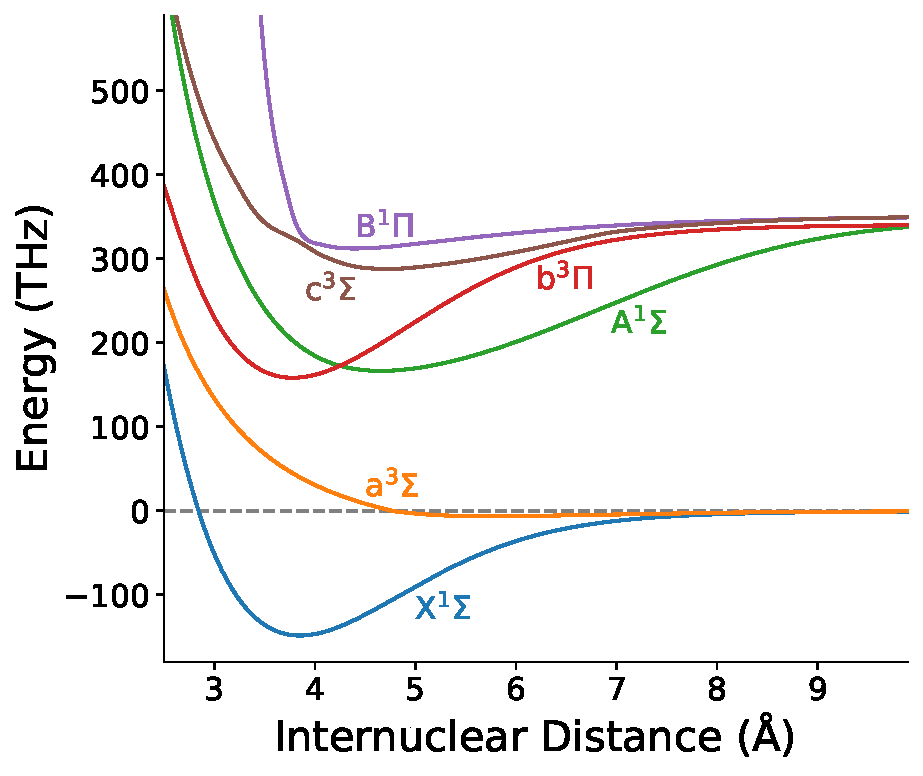
\includegraphics[width=0.9\textwidth]{figures/pa_pes.pdf}
  \caption[NaCs potential energy surfaces]{
    Potential energy surfaces of NaCs with \textit{Hund's~case~(a)} labels.
    Due to spin-orbit coupling, the potentials are not independent of each other.
    The real energy eigenstates of the molecule may be a superposition of multiple
    electronic and spin states.
    \label{fig:pa:pes}}
\end{figure}

Fig.~\ref{fig:pa:pes} shows the relevant PESs for $\mathrm{NaCs}$.
Although the spin-less electronic Hamiltonian~\ref{eq:pa:pes:he} makes it easier
to understand the molecule structure and provides good approximations for the
transition dipoment and FCF, the absense of spin and the difficulty in exactly solving
a multi-electron system makes it unsuitable to calculate energy levels
for spectroscopy purpose.
Because of this, prediction of the molecular states energies are calculated using
PESs fitted to experimental data~\cite{docenko_coupling_2006,zaharova_solution_2009,grochola_spin-forbidden_2011,grochola_investigation_2010}.

\section{Photoassociation Spectroscopy}
\label{ch:pa:pa}

\subsection{Beampath}
\label{ch:pa:beampath}

\begin{figure}
  \centering
  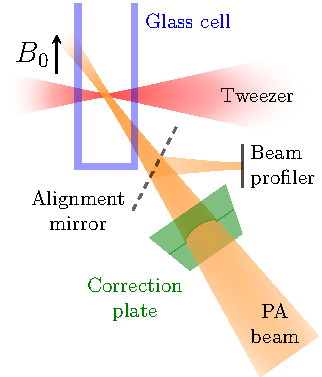
\includegraphics[width=0.7\textwidth]{figures/pa_beampath.pdf}
  \caption[PA beampath]{
    PA beampath including the relative geometry with the magnetic field
    the glass vacuum cell and the tweezer.
    In order to compensate for the astigmatism from pass through the glass cell window
    at an angle, we added an correction glass plate into the PA beam path.
    The correction plate has the same thickness and angle of incident with the glass cell window
    but is angled vertically instead of horizontally.
    The alignment mirro and the beam profiler can also be added to the beam path
    in order to measure the chromatic error during alignment.
    \label{fig:pa:beampath}}
\end{figure}

The excited molecular state we would like to address has a bond length of $3-8~\mathrm{\AA}$.
The initial atomic state, however, has an average inter-nuclear distance of
$\approx1000~\mathrm{\AA}$.
This size mismatch between the initial and final state wavefunctions
means the transition typically have a very small FCF~($10^{-10}-10^{-8}$).
Because of this, we focus our PA beam onto the tweezer with a beam waist between
$10~\mathrm{\mu m}$ and $30~\mathrm{\mu m}$~(Fig.~\ref{fig:pa:beampath}) in order to
increase the laser intensity and improve the signal contrast.
The tight focus also increase the astigmatism when passing through
the glass cell window at an angle which limits the minimum focus size we can achieve.
Therefore, we added a correction glass plate to fix the astigmatism
in order to minimize the focus size and maximize the beam intensity.

\begin{figure}
  \centering
  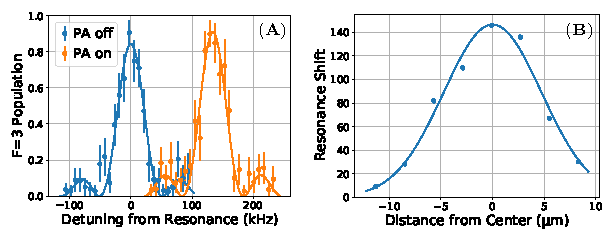
\includegraphics[width=\textwidth]{figures/pa_vectorshift.pdf}
  \caption[PA beam alignment]{
    Measurement of Cs vector light shift from the PA beam for final alignment.
    (A) The effective magnetic field from the circularly polarized PA beam
    causes a shift on the Raman resonance between the $|4,4\rangle$ and $|3,3\rangle$ states.
    (B) Vector light shift as a function of PA beam position
    used to determine the beam center.
    The $1/\ue$ diameter of the beam is measured to be $13.40(72)~\mathrm{\mu m}$.
    \label{fig:pa:alignment}}
\end{figure}

In order to align the PA beam to the tweezer, we use the following alignment procedure,
\begin{enumerate}
\item Light resonant with the Cs atomic transition is sent into the PA beam path.
  This allows us to do the alignment using the procedure we used to align the
  atomic Raman sideband cooling beams as described in section~\ref{ch:rsc:alignment}.
  However, unlike the alignment for the atomic Raman beams,
  due to the larger frequency difference between the PA transition and the Cs atomic
  transition as well as the smaller beamsize,
  we cannot use the alignment result from this step directly for the PA beam
  due to the chromatic aberration from the optics in the PA beam path.
\item In order to translate the alignment result from resonance Cs light to that of the PA light,
  we insert a mirror to reflect the PA beam after the last optics in the beam path
  and place a beam profiler at the equivalent location of
  the tweezer~(Fig.~\ref{fig:pa:beampath}).
  This allow us to directly measure location of the focal point for the two wavelengths
  and correct for the chromatic aberration by shifting the focus from the PA light
  to the original focus position from the resonance Cs light.
\item As the final alignment step and to correct for the chromatic aberration of the
  glass window that was not corrected for in the last step,
  we align the PA beam to the atom using signal directly from the atom.
  Due to the large detuning, the scattering rate from the PA beams
  is too low to be used for alignment.
  However, when the PA beam is set to circular polarization, it creates an effective
  magnetic field parallel to the beam propagation direction
  of the form~\cite{thompson_coherence_2013},
  \[ B_{\mathrm{eff}}=-U_0\frac{\delta_2-\delta_1}{\delta_2+2\delta_1}\mathbf{C} \]
  where $U_0$ is the scalar light shift, $\delta_1$ and $\delta_2$ are the detuning from the
  $\mathrm{D}_1$ and $\mathrm{D}_2$ line respectively,
  $\mathbf{\varepsilon}$ is the polarization vector and
  $\mathbf{C}\equiv\Im\paren{\mathbf{\varepsilon}\times\mathbf{\varepsilon}^*}$
  qualifies the ellipticity of the polarization with
  $\abs{C}=1$ for pure circular polarization and $\abs{C}=0$ for linear polarization.
  This effective magnetic field causes a relative shift between the $|4,4\rangle$
  and the $|3,3\rangle$ states which can be measured using
  a Raman transition~(Fig.~\ref{fig:pa:alignment}A).
  By measuring the shift as a function of the beam position,
  we can determine the size and the center of the PA beam and align the beam to
  the atom~(Fig.~\ref{fig:pa:alignment}B).
\end{enumerate}

\subsection{Experiment Sequence and Resonance Frequencies}
\label{ch:pa:sequence-res}

\begin{table}
  \centering
  \begin{tabular}{|c|c|c|c|c|}
    \hline
    Vibrational State&$v'=0$&$v'=12$&$v'=13$&$v'=14$\\\hline
    Resonance Prediction (GHz)&$288722$&$306491$&$307876$&$309252$\\\hline
  \end{tabular}
  \caption[PA resonance prediction]{
    Prediction of $|\mathrm{Na(2, 2),Cs(4, 4)}\rangle$ PA resonance frequency
    based on Dunham expansion~\cite{grochola_spin-forbidden_2011,dunham_energy_1932}.
    \label{table:pa:theory-prediction}}
\end{table}

For the PA spectroscopy, we mainly focus on states with large binding energies
which are expected to be good candidates as the intermediate state
for Raman transfer~(section~\ref{ch:raman-transfer:raman}).
In particular, we scanned the PA light frequency around the $v'=0$ and $v'=12-14$
vibrational states in the $c^3\Sigma_{\Omega=1}$ potential.
Table~\ref{table:pa:theory-prediction} shows the predicted resonance frequencies
for the PA resonance from $|\mathrm{Na(2, 2),Cs(4, 4)}\rangle$
based on fitting to previous measurement~\cite{grochola_spin-forbidden_2011}.
The frequencies are calculated from Dunham expansion~\cite{dunham_energy_1932}
corrected for the hyperfine structure for the atoms.

In order to observe PA, we first prepare both the Na and Cs atoms in the motional ground states
in the same tweezer~\cite{liu_building_2018}.
We then turn on the PA beam for a set time
followed by separating the atoms into their respective tweezers and image the atoms.
When we hit a PA resonance, the excited molecular state will typically decay down
to either a molecular ground state,
which will remain in at most one of the tweezers after the separation,
or an atomic state with high relative motional energy and escape the trap.
In either case, this leads to at least one empty tweezer after the separation.
By measuring the probability of having both the Na and Cs atoms after the PA pulse
conditioned on both atoms being initially loaded,
we can capture the probability of PA event and locate the resonances.

The initial atomic state we used is $|\mathrm{Na(2, 2),Cs(4, 4)}\rangle$
which has $L=0$ and $S=1$.
For atoms in the motional ground state we also have $N=0$ and therefore $J=1$
which should be coupled to $J=0,1,2$ excited states from the $\Delta J=0,\pm1$ selection rule.
However, since the cooling is not perfect,
we expect some atoms initially in the $N=1$ state which can allow a weaker
transition to the $J=3$ states.
Moreover, since the PA beam polarization is circular
and has maximum overlap with the $\sigma^+$ polarization,
the $J=2$ is expected to have the strongest coupling.

\begin{figure}
  \centering
  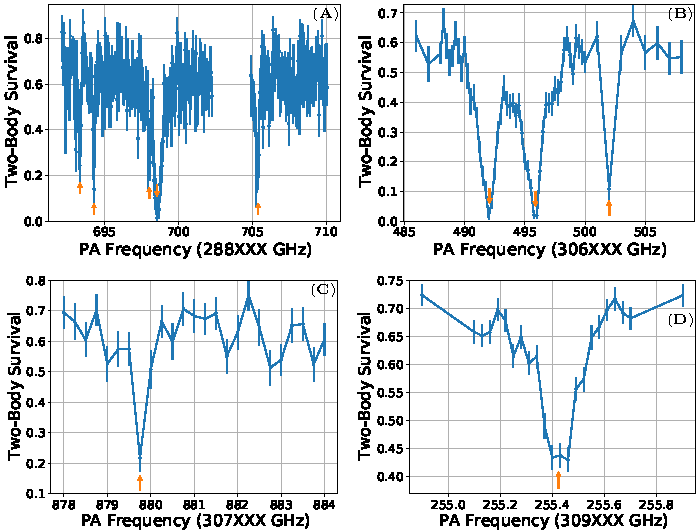
\includegraphics[width=\textwidth]{figures/pa_spectrum.pdf}
  \caption[PA spectrum]{
    PA spectrum for (A) $v'=0$, (B) $v'=12$, (C) $v'=13$, (D) $v'=14$.
    The PA frequency is shown in GHz with an offset.
    Multiple rotational states can be observed for $v'=0$ and $v'=12$.
    $v'=0$ also shows multiple peaks that corresponds to
    the hyperfine structure of the molecule.
    The $v'=13$ and $v'=14$ transitions are relatively weak
    and only the strongest line is measured as a result.
    \label{fig:pa:spectrum}}
\end{figure}

\begin{table}
  \centering
  \begin{tabular}{|c|c|c|c|c|c|}
    \hline
    \multicolumn{2}{|c|}{Vibrational State}&$v'=0$&$v'=12$&$v'=13$&$v'=14$\\\hline
    \multirowcell{5}{Resonance\\(GHz)}&\multirowcell{2}{$J=1$}&$288693.3$&$306492.1$&-&-\\\cline{3-6}
    {}&&$288694.3$&-&-&-\\\cline{2-6}
    {}&\multirowcell{2}{$J=2$}&$288698.0$&$306495.9$&$307879.8$&$309255.4$\\\cline{3-6}
    {}&&$288698.5$&-&-&-\\\cline{2-6}
    {}&$J=3$&$288705.4$&$306502.0$&-&-\\\hline
  \end{tabular}
  \caption[PA resonance frequencies]{
    PA resonance frequencies for $v'=0,12-14$.
    The $J$ numbers for $v'=0$ and $v'=12$ are assigned based on the rotational state spacing.
    For $v'=13$ and $v'=14$, we assume the observed line is $J=2$
    which is expected to be have the strongest coupling.
    \label{table:pa:all-lines}}
\end{table}

Fig.~\ref{fig:pa:spectrum} shows the PA spectra measured for different vibrational states
with the frequencies summarized in table~\ref{table:pa:all-lines}.
The spectra for $v'=0$ and $v'=12$ shows three rotational states
whereas only the strongest rotational state is measured for $v'=13$ and $v'=14$.
The $v'=0$ spectrum also shows the hyperfine structure for the lowest two rotational states.

The rotational states of the molecule can be determined from the energy gap between the states
based on the discussion in section~\ref{ch:pa:angular-momentums:deep}.
The ratio of the spacing between the lowest $J$ states we measured are
$1.64$ and $1.61$ for $v'=0$ \footnote{The energy of the strongest hyperfine line is used}
and $v'=12$ respectively.
This is very closed to the ratio of $3/2$ for $\Omega=1$ states.
The main source of the deviation is likely the hyperfine structure
that was ignored in the discussion above.

\subsection{Linewidth}
\label{ch:pa:linewidth}

In additional to the energy, another property of the excited state
that is important for driving a two-photon transition using the state is the linewidth.
This determines the scattering or decoherence rate of
the two-photon transition which then determines
the transfer efficiency~(chapter~\ref{ch:raman-transfer}).
The linewidth, or decay rate, due to electric dipole transitions
is~\cite[p.~197]{bransden_physics_2003},
\begin{align*}
  \Gamma=&\sum_{i}\frac{\omega_i^3d_i^2\mathrm{FCF}_i}{3\pi\varepsilon_0\hbar c^3}
\end{align*}
where $\omega_i$ is the decay frequency, $d_i$ is the transition dipole moment,
and the sum is over all the decay channels.
Since the size of the excited state electron wavefunction is similar to that of the atom
the molecule has a similar transition dipole moment as the corresponding atomic transition
$d_i\approx d_\Cs$. Moreover, since $\sum_i\mathrm{FCF}_i=1$ and $\omega_i\approx\omega_\Cs$
we have
\begin{align*}
  \Gamma\approx&\frac{\omega_\Cs^3d_\Cs^2}{3\pi\varepsilon_0\hbar c^3}\\
  =&\Gamma_\Cs\approx2\pi\cdot5~\mathrm{MHz}
\end{align*}
Since the PA laser is locked using a wavemeter with a precision
$\approx20~\mathrm{MHz}$, we expect the PA linewidth we measured to be limited
by our frequency resolution.

\begin{figure}
  \centering
  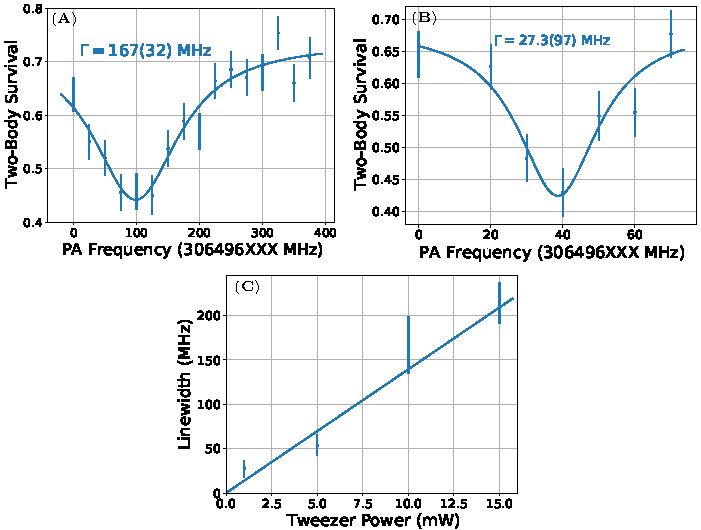
\includegraphics[width=\textwidth]{figures/pa_linewidth_red_twr.pdf}
  \caption[PA linewidth for red detuned tweezer]{
    Fitting of PA linewidth for (A) $10~\mathrm{mW}$, (B) $1~\mathrm{mW}$ tweezer power,
    showing a broad linewidth and a significant difference between the two.
    (C) Fitting of the PA linewidth as a function of tweezer power suggests
    a proportional relation between the two.
    \label{fig:pa:linewidth:red-twr}}
\end{figure}

This is, however, not what is observed in the experiment.
Fig.~\ref{fig:pa:linewidth:red-twr}A shows the narrowest spectrum of the $v'=12, J=2$ PA line
we measured when the tweezer frequency is set to $306344.~\mathrm{GHz}$
with $10~\mathrm{mW}$ of power. The linewidth is determined to be $167(32)~\mathrm{MHz}$
which is much greater than the theory prediction.

Furthermore, the observed linewidth appears to be dependent on the tweezer power.
The same PA line measured with $1~\mathrm{mW}$ tweezer power
is shown in Fig.~\ref{fig:pa:linewidth:red-twr}B with a significantly narrower linewidth
of $27.3(97)~\mathrm{MHz}$.
In fact, the linewidth appears to be proportional to the tweezer power
as shown in Fig.~\ref{fig:pa:linewidth:red-twr}C,
which suggests that the linewidth may be broadened by a two-photon process.

\begin{figure}
  \centering
  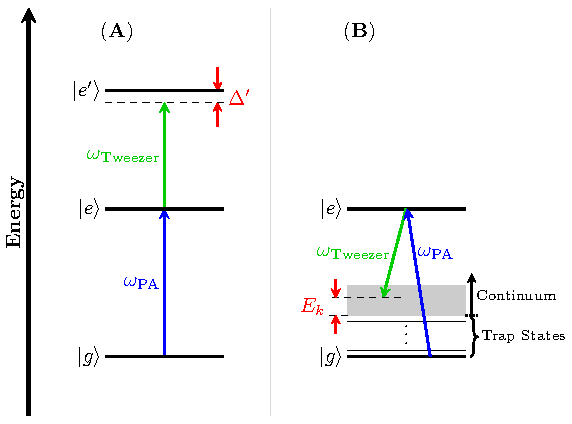
\includegraphics[width=0.939\textwidth]{figures/pa_two_photon_up_vs_down.pdf}
  \caption[Two-photon broadening mechanism for PA.]{
    Potential two-photon broadening mechanism for PA by coupling the excited state $|e\rangle$
    via the tweezer to (A) a higher excited state $|e'\rangle$ or
    (B) the atomic motional continuum.
    (A) For coupling to a higher excited state,
    the broadening depends on the two-photon detuning $\Delta'$ from $|e'\rangle$.
    (B) For coupling to the atomic motional continuum,
    the broadening is a function of the kinetic energy of the atomic state $E_k$.
    \label{fig:pa:linewidth:up-vs-down}}
\end{figure}

We initially suspected that the source of this broadening is due to the tweezer light
coupling the excited molecular state to another state at
a higher energy~(Fig.~\ref{fig:pa:linewidth:up-vs-down}A).
If this is the case, we would expect the broadening to be a function of
the sum of the tweezer and PA light frequency depending on the detuning from the nearest
two-photon excited state.
However, the broadening does not change significantly when the tweezer frequency
is changed by $\approx10~\mathrm{GHz}$ and
is also observed for other excited states including $v'=0$ and $v'=14$
which have very different resonance frequencies.
It is therefore unlikely that this is the broadening mechanism we observe.
Instead, we believe the effect is caused by a $\Lambda$ type two-photon process
coupling the excited state to the atomic ground states.
In the following section, I will provide an estimation for such a broadening process.

\subsubsection{Two-Photon Coupling to the Atomic Motional Continuum}
The broadening of the PA line requires coupling the excited state to a continuum of states.
For the ground atomic state, since the state is stable with repect to radiative decay,
this continuum cannot be the photon continuum.
Instead, the excited state is coupled to the relative motional continuum of the atoms.
Physically, this corresponds to a photodissociation process
where the atoms flies away with high kinetic energies corresponding
to the detuning of the tweezer~(Fig.~\ref{fig:pa:linewidth:up-vs-down}B).

The photodissociation rate is determined by the Fermi's golden rule,
\[
  \Gamma=2\pi\Omega_{if}^2\ \rho_f
\]
where $\Omega_{if}$ is the matrix element between the initial and final state
and $\rho_f$ is the density of state near the final state.
We calculate this by first discretizing the continuum and the rate becomes
\[
  \Gamma=2\pi\frac{{\Omega'_{if}}^2}{\delta}
\]
where $\Omega'_{if}$ is the Rabi frequency between the initial and final state
and $\delta$ is the spacing between the discretized final states.

The Rabi frequency $\Omega'_{if}$ is proportional to the square root of FCF,
which we calculate for the atomic ground motional states by exactly diagonalization
of the atomic wavefunction.
However, due to the high energy~($>10~\mathrm{GHz}$) of the final state,
calculating FCF for the target state using this method requires an unrealiztic number of
states to be included.
Instead, we approximate it using the results for the atomic ground state
by assuming the FCF to be proportional to the probability density of non-interacting
atomic wavefunction at zero relative distance so that,
\[
  \Omega'_{if}=\Omega_0\frac{\psi_f\paren{r_{rel}=0}}{\psi_0\paren{r_{rel}=0}}
\]
where $\Omega_0$ is the Rabi frequency between the excited state and
the atomic motional ground state and $\psi_f$ and $\psi_0$ are the
wavefunctions of the final and ground motional atomic state without the molecular potential.
This approximation is justifed because,
\begin{enumerate}
\item The molecular potential is short ranged and the excited molecular state is small.
\item Only the final atomic wavefunction within the molecular potential contributes to the FCF.
  For relatively low motional energy
  this wavefunction is proportional to the value of the wavefunction at
  the edge of the molecular potential which is well approximated by
  the atomic wavefunction without the molecular potential.
\end{enumerate}
This approximation remains valid until the de Broglie wavelength for the atomic state
is comparable to the size of the molecular potential which corresponds to
a motional energy of $\approx40~\mathrm{GHz}$
and the result can still be used as order of magnitude estimation for higher motional energies.

For atomic motional ground state, we have,
\begin{align*}
  \psi_0\paren{r_{rel}=0}=&\prod_{i=1}^{3}\paren{\frac{\mu\omega_i}{\pi}}^{1/4}\\
  =&\paren{\frac{\mu^3\omega_1\omega_2\omega_3}{\pi^3}}^{1/4}
\end{align*}
where $\mu$ is the reduced mass $\mu\equiv m_\Na m_\Cs/\paren{m_\Na+m_\Cs}$,
and $\omega_i$'s are the relative trapping frequencies along the three trap axis.
We discretize the continuum state by adding an infinitely deep spherical potential well
of radius $R$ around the center. The radial wavefunctions of the eigenstates
within the well with quantum number $n=1,2,\dots$ is,
\begin{align*}
  \psi_n=&\frac{1}{\sqrt{4\pi}r_{rel}}\sqrt{\frac{2}{R}}\sin\paren{\frac{\pi nr_{rel}}{R}}
\end{align*}
and the corresponding energy,
\begin{align*}
  E_n=&\frac{\pi^2n^2}{2\mu R^2}
\end{align*}
The energy gap between neighboring states is
\begin{align*}
  \delta_n\approx&\frac{\pi^2n}{\mu R^2}
\end{align*}
and the wavefunction value at $r_{rel}=0$ is,
\begin{align*}
  \psi_n\paren{r_{rel}=0}=&\sqrt{\frac{1}{2\pi R}}\left.\frac{\ud}{\ud r_{rel}}\sin\paren{\frac{\pi nr_{rel}}{R}}\right|_{r_{rel}=0}\\
  =&\frac{\pi n}{\sqrt{2\pi R}R}
\end{align*}
Substituting into $\Gamma$ and taking the limit of $R\rightarrow\infty$ we have
\begin{align*}
  \Gamma=&2\pi\frac{\Omega_0^2}{\delta}\frac{\psi_f^2\paren{r_{rel}=0}}{\psi_0^2\paren{r_{rel}=0}}\\
  =&2\pi\Omega_0^2\frac{\mu R^2}{\pi^2n}\frac{\pi^2 n^2}{2\pi R^3}\sqrt{\frac{\pi^3}{\mu^3\omega_1\omega_2\omega_3}}\\
  =&\Omega_0^2\frac{n}{R}\sqrt{\frac{\pi^3}{\mu\omega_1\omega_2\omega_3}}\\
  =&\Omega_0^2\sqrt{\frac{2\pi E}{\omega_1\omega_2\omega_3}}
\end{align*}
For the condition in Fig.~\ref{fig:pa:linewidth:red-twr}A
we have $\Omega_0=2\pi\cdot\todo{number}...$,
$E=2\pi\cdot\todo{number}...$ and $\omega_{1,2,3}=2\pi\cdot\todo{number}...$
which predicts a broadened linewidth of $\Gamma=2\pi\cdot\todo{number}...$.
This prediction is only an estimate due to the breakdown of the approximation
we used and is in fact broader than the observed value.
Nevertheless, it confirms that this broadening mechanism can explain the observed linewidth.

\todo{Acknowedge Olivier}

\subsubsection{Eliminating the Broadening with Blue Detuned Tweezer}

\begin{figure}
  \centering
  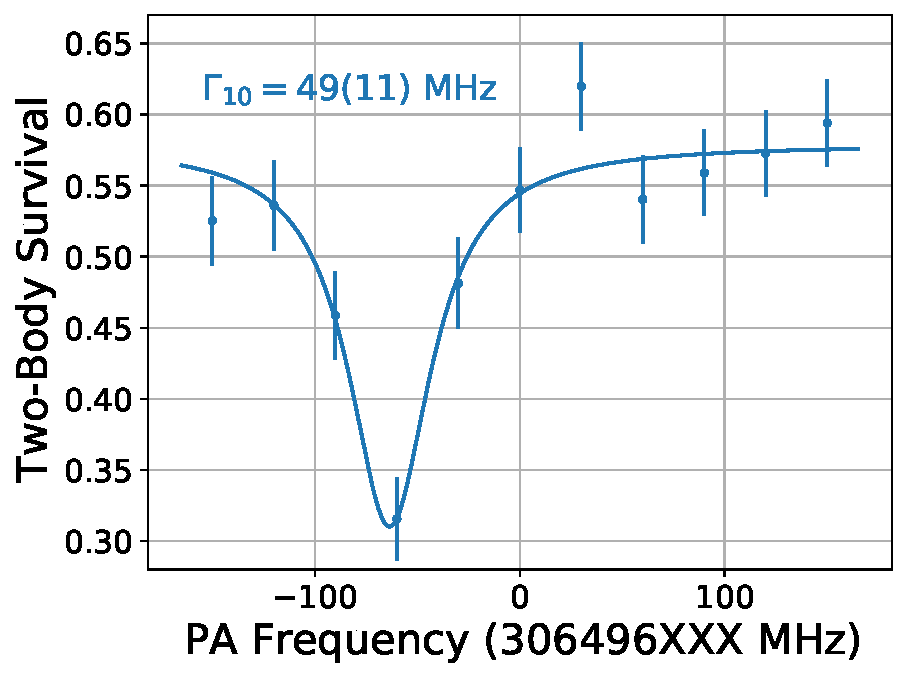
\includegraphics[width=0.55\textwidth]{figures/pa_spectrum_v12_blue_10.pdf}
  \caption[PA linewidth for blue detuned tweezer]{
    Fitting of PA linewidth for $10~\mathrm{mW}$ tweezer power at $306612~\mathrm{GHz}$.
    The linewidth is significantly narrower than the value measured when the tweezer
    is red detuned from the PA resonance~(Fig.~\ref{fig:pa:linewidth:red-twr}).
    \label{fig:pa:linewidth:blue-twr}}
\end{figure}

Another prediction from the theory is that if the tweezer light is blue detuned from
the PA line, the two-photon process will not couple to the motional continuum anymore
and there should be no broadening of the line
\footnote{Note that the tweezer is still red detuned from the atomic state which
  provides most of the trapping potential}.
We can confirm this by measuring the linewidth of the same PA line with the tweezer
frequency set to $306612~\mathrm{GHz}$.
The result shown in Fig.~\ref{fig:pa:linewidth:blue-twr}
confirms that the linewidth is indeed narrower for this tweezer frequency.

\subsubsection{Implication on Two-Photon Transition to Ground Molecular States}

\begin{figure}
  \centering
  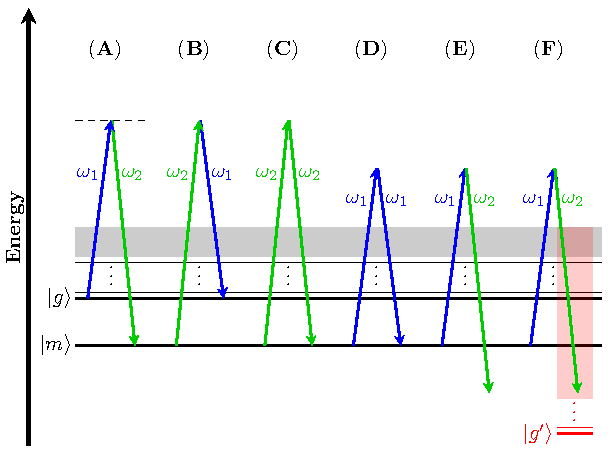
\includegraphics[width=\textwidth]{figures/pa_two_photon_down_raman.pdf}
  \caption[Two-photon transition from molecular state.]{
    Effect of two-photon coupling to atomic contimuum on molecular state.
    (A) Raman transition from the atomic ground state $|g\rangle$
    to the molecular bound state $|m\rangle$ using two Raman beams with frequencies
    $\omega_1$ and $\omega_2$.
    (B-E) Two photon transitions starting from the molecular state $|m\rangle$
    with different frequency combinations without additional atomic spin states.
    (B) This is the reverse Raman transition and reaches the initial atomic state.
    (C,D) The frequency pairs couples back to $|m\rangle$.
    (E) This couples to an energy below $|m\rangle$.
    Note that none of the two-photon transitions from $|m\rangle$ in (B-E) ends up in
    the atomic motional continuum and therefore unaffected by the broadening mechanism
    discussed in this section.
    (F) The present of another atomic spin state $|g'\rangle$ with lower energy
    allows the two-photon transition from $|m\rangle$ to be coupled to the
    motional continuum corresponding to the new spin state.
    Note that only the frequency combination similar to (E) is shown for simplicity,
    other cases may also couple to the same continuum.
    \label{fig:pa:linewidth:two-photon-down-raman}}
\end{figure}

Since the broadening is caused by two-photon coupling to high energy atomic motional states,
the observed linewidth in a PA measurement cannot be directly translated to
the scattering rate during a two-photon transition that uses different set of laser frequencies.

In fact, with a single ground atomic spin state, the scattering rate for the final molecular
state during a two-photon transition is not affected by this effect.
As shown in Fig.~\ref{fig:pa:linewidth:two-photon-down-raman}B-E,
the molecular state cannot reach the atomic motional continuum via a two-photon transition.
The atomic state, on the other hand, can reach the continuum though the loss rate is in general
much lower than the molecular state
and is usually not the limiting factor for the transfer efficiency.

The molecular state can also couple to a different motional continuum if there are other
atomic spin state with lower energy~(Fig.~\ref{fig:pa:linewidth:two-photon-down-raman}F).
Since stable atomic state has the lowest energy amount all the ones with the same total $m_F$,
such state must have a different total $m_F$ than the initial state.
Therefore, such coupling is forbidden if the two Raman beams both has $\pi$ polarization,
as is the case for the Raman transition in chapter~\ref{ch:raman-spectroscopy}
and \ref{ch:raman-transfer}, and will not cause any loss due to this mechanism.
Polarization impurity, however, can allow such coupling and enable this loss process.

\section{Summary and Outlook}
We continued our study of the interaction between two atoms in the optical tweezer.
We characterized the excited molecular potential by measuring
the energy of bound states using photoassociation spectroscopy
and identified the states based on their rotational structure.
On the other hand, the high intensity of the optical tweezer
also creates unique challenges that can lead to dissociation or loss of the atoms or molecules.
We studied one of the effect and confirmed our model for the loss process with
additional measurements and discussed its implication for future experiment.
The identification of the excited molecular state opens up the pathway
to formation of ground state single molecule via two-photon process
and will be focus of later chapters.

% Two-photon spectroscopy of NaCs ground state
% -*- mode: latex-mode; TeX-engine: xetex; LaTeX-command-style: (("" "SOURCE_DATE_EPOCH=0 %(PDF)%(latex) --shell-escape %S%(PDFout)")); TeX-master: "../dissertation.tex"; -*-

\chapter{Two-photon Spectroscopy of NaCs Ground State}
\label{ch:raman-spectroscopy}

\section{Introduction}

\todo{make sure the goal of reaching the absolute ground state is stated previously.}

The excited molecular states measured and characterized in chapter \ref{ch:pa}
provide us a pathway to couple to the ground electronic molecular states
using two-photon transitions.
While it is in principle possible to drive from the atomic state
to any desired molecular ground state for various applications,
doing so directly has many technical challenges.
We will cover these challenges as well as the considerations in selecting
the molecule formation pathway in chapter \ref{ch:raman-transfer},
however, the difficulty, and the main difference from a pure atomic Raman transition,
lies in the wavefunction size mismatch.
As we have seen already in section \ref{pa:beampath},
the size mismatch between the excited molecular states and the ground atomic state
causes a very small FCF and requires a high PA intensity to improve the signal strength.
This small FCF also reduces the Rabi frequency for the two-photon transition to the ground state.
As a result, driving a two-photon transition to an arbitrary molecular ground state
may require maintaining coherence between two different lasers over
a relatively long time (milliseconds) which is very difficult to achieve.

Our solution to this challenge is to do the transfer via a two step process.
\begin{enumerate}
\item We drive a two-photon transition from the atomic state to
  a weakly bound ground state.
  The reduced energy difference allows the laser coherence to be maintained
  over a longer time easily.
  In the case of NaCs molecule, this also increases the FCF
  between the ground and excited molecular states which allows shorter pulse time and
  further reduces the coherence requirement.
\item The transfer to arbitrary molecular ground state will be done from
  the weakly bound state created in the first step.
  The strength of this transition can be much higher
  and only requires a relatively shorter laser coherence time.
  This step has already been demonstrated in other experiments\todo{\cite{}}
  so in this thesis we will focus only on the first step transfer.
\end{enumerate}

In this chapter, we will discuss the use of Raman spectroscopy
to measure the properties of the weakly bound molecular ground states.
In section \ref{ch:raman-spectroscopy:states}
we will describe the states involved and the setup for the Raman spectroscopy
as well as the measured binding energy for the $N=0$ states.
In section \ref{ch:raman-spectroscopy:n2}
we study the coupling between angular momentums for near threshold molecular states
by characterizing the $N=2$ states.

\section{Weakly bound NaCs Ground States}
\label{ch:raman-spectroscopy:states}

As mentioned in section \ref{pa:structure:near-threshold},
the angular momentum coupling for weakly bound molecular state is similar to that of the atoms.
Therefore, instead of using the term symbol for the \textit{Hund's case (a)}
to identify the molecular potential and bound states,
we use the hyperfine state ($F_{Na}, F_{Cs}$) for the atoms instead.
Similarly, since the vibrational states of the molecule does not always corresponds to
a particular short range potential, we also label the vibrational states
from the the atomic state threshold.
Under this system, the atomic motional ground state is $v''=0$ and
the first (lowest binding energy) molecular bound state is $v''=-1$.

\todo{figure?}
In order to measure the binding energy of a molecular state,
we first prepare the atom in the corresponding hyperfine state
and drive a Raman transition to the molecular state.
We use a Raman transition that is detuned from the $c^3\Sigma\ v'=0$ state measured
in section \ref{pa:pa}.
\todo{Maybe move stable HF combination to interaction shift?}
When the Na and Cs are in the same tweezer,
they can undergo fast spin-exchange collision that changes the hyperfine state of the atom.
This process can cause the hyperfine energy ($>1\mathrm{GHz}$) of the atoms
to be transferred to the motional energy
and eject the atoms from the tweezer ($<100\mathrm{MHz}$ deep).
As a result, the measurement can only be done when the spin-exchange collision is suppressed,
which includes the following spin combinations,
\begin{enumerate}
\item $F_{Na}=1$ and $F_{Cs}=3$\\
  This is the spin state with the lowest energy and therefore the spin-exchange interaction
  is energetically forbidden.
  In the experiment, we use the state $|Na(1, 1),Cs(3, 3)\rangle$
  which can be prepared from the $|Na(2, 2),Cs(4, 4)\rangle$ state from OP
  easily by driving a Raman transition for both Na and Cs atoms.
  This state also remains the lowest energy atomic state in the present of a weak magnetic field.
\item $|Na(2, 2),Cs(4, 4)\rangle$ and $|Na(2, 2),Cs(3, 3)\rangle$
  \footnote{States with opposite $m_F$, i.e.
    $|Na(2, -2),Cs(4, -4)\rangle$ and $|Na(2, -2),Cs(3, -3)\rangle$ are also stable
    but are omitted here since these cannot be easily prepared in our experiment.}\\
  These spin states are stable because the spin-exchange collision conserves total $m_F$
  of the two atoms and
  the two states are the lowest energy states that has the same total $m_F$.
  Inelastic collision that changes the total $m_F$ can also happen
  but has a lower collision rate since it requires transferring angular momentum
  between the spin and motion of the atom.
\end{enumerate}

\subsection{Driving Raman Transition using the Optical Tweezer}

\begin{figure}
  \centering
  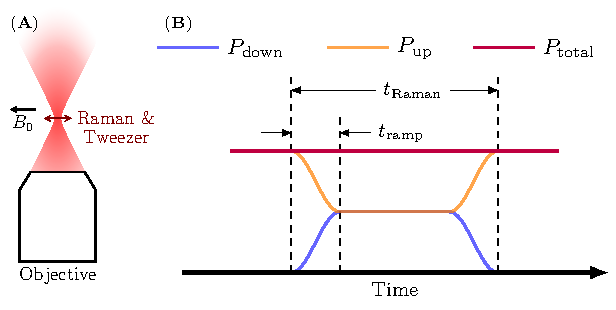
\includegraphics[width=\textwidth]{figures/raman_spectroscopy_apparatus_sequence.pdf}
  \caption[Raman transition setup and sequence]{
    (A) Geometry and polarization of trap and Raman beam relative to the bias magnetic field.
    We use a bias B field of $B_0=8.8 G$ alone the tweezer polarization
    to define the quantization axis
    which is the same as the one used for Raman sideband cooling in Fig.~{fig:na-rsc-geometry}.
    As a result, the atoms experiences predominately $\pi$ polarization from the tweezer.
    (B) Raman transition pulse sequence.
    The tweezer initially consists of only up leg power.
    When driving the Raman transition, the up leg power is smoothly ramped down and
    the down leg power ramped up over $t_{ramp}=10\mathrm{\mu s}$
    while maintaining the total power of the tweezer.
    This minimizes the heating on the atoms due to power fluctuation while maximizes the time
    with maximum Raman Rabi frequency when the up and down leg powers are equal.
    \label{fig:raman-spectroscopy:apparatus-sequence}}
\end{figure}

\begin{figure}
  \centering
  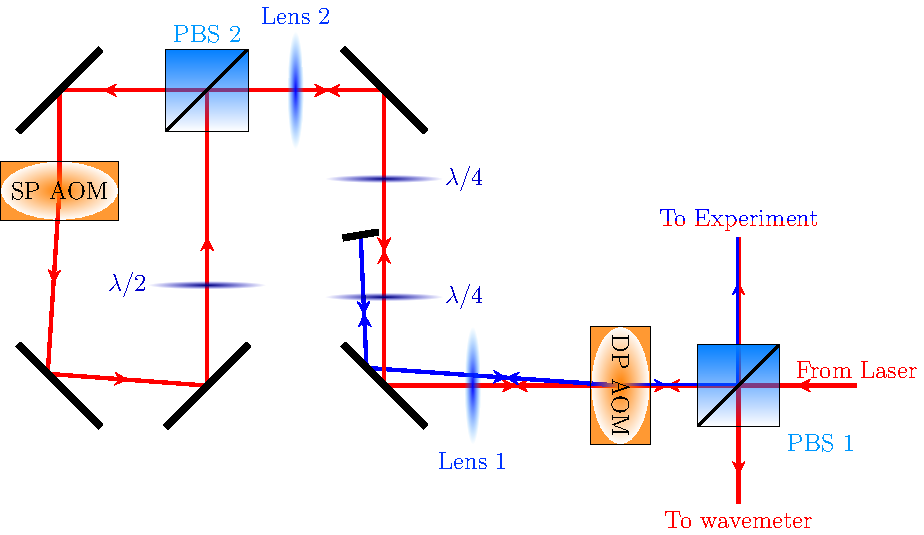
\includegraphics[width=\textwidth]{figures/raman_spectroscopy_raman_beampath.pdf}
  \caption[Beampath to allow driving Raman transition with tweezer]{
    Beampath for generating the frequency for Raman transition in the tweezer.
    (Beampath for fiber coupling and overall power control is not shown.)
    The red beam path is the $0$-th order of the double pass (DP) AOM
    which is used for the tweezer.
    When the DP AOM is turned on, some power is redirected to the first order
    (blue beam path) which generates the required frequency different to drive
    the Raman transition. The two frequencies are recombined on the DP AOM.
    The $0$-th order light is shifted by another single pass (SP) AOM
    running on a different frequency before recombining.
    Without this AOM, the leak light from the DP AOM will be at the same frequency
    as the $0$-th order light which can cause a significant power fluctuation
    due to interference. The SP AOM ensures that none of the leaking light frequency
    coincide with either intended frequencies therefore avoiding this issue.
    Different selection of the SP and DP AOM as well as their orders can be used
    to cover a wide range of two photon detuning for Raman transition.
    The experiment typically start with the SP AOM on and the DP AOM off.
    When driving the Raman transition, the powers on both AOMs are ramped simultaneously
    to achieve the desired power at both frequencies.
    \label{fig:raman-spectroscopy:raman-beampath}}
\end{figure}

In order to increase the intensity of the Raman beams to overcome the small FCF,
we use the tweezer beam to drive the Raman transition
(Fig.~\ref{fig:raman-spectroscopy:apparatus-sequence}A).
Not only does this maximizes the intensity due to the small focal size of the tweezer,
since the atoms are trapped at the maximum of the tweezer beam,
this also ensures that the Raman beam is aligned automatically to the atoms
and suppresses sensitivity to mechanical fluctuation that is usually
caused by a small beam size.
Moreover, this also minimizes the number of beams the atoms experience
during the Raman transition which, in turns, minimizes the scattering.
As a result, the coherence of the transition is also improved
which is important for achieving coherent creation of molecule
(chapter \ref{ch:raman-transfer}).

The beampath to generate the required frequencies in the tweezer is shown in
Fig.~\ref{fig:raman-spectroscopy:raman-beampath}.
The additional single pass AOM in the beampath avoids interference
with AOM leak light causing power fluctuation and
also increases the frequency tuning range compared to using only one double pass AOM.
The powers at each frequencies are calibrated as a function of AOM powers
so that we can select the desired power ratio during the experiment.
When driving the Raman transition, instead of turning on separate beam,
we ramp down the power at the original tweezer and ramping up the power
in the second frequency while maintaining the total power to minimize heating of the atoms
(Fig.~\ref{fig:raman-spectroscopy:apparatus-sequence}B).

\subsection{Raman Resonance on $N=0$ Ground State}

\begin{figure}
  \centering
  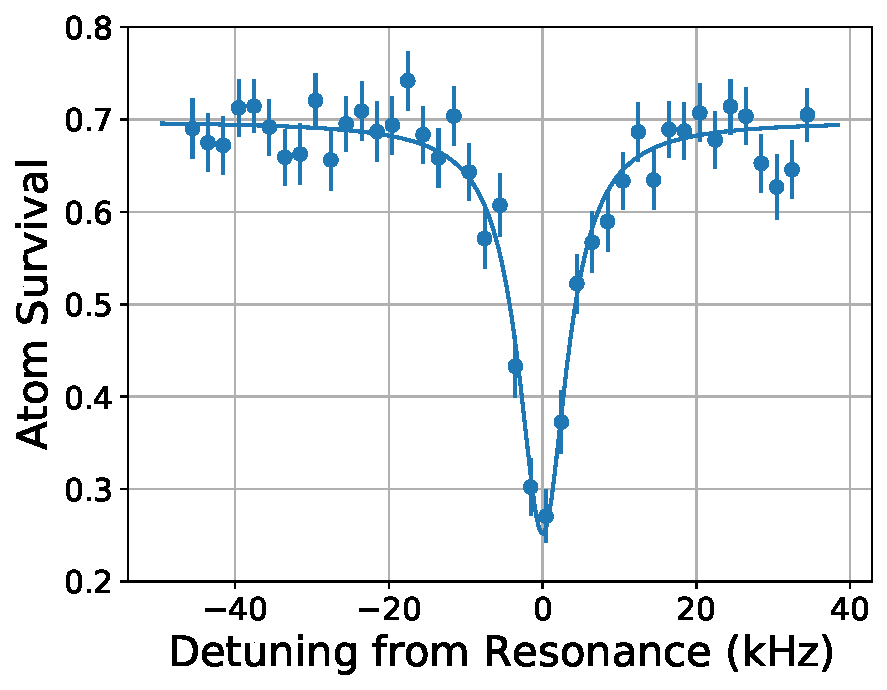
\includegraphics[width=0.7\textwidth]{figures/raman_spectroscopy_resonance.pdf}
  \caption[Raman resonance for $v''=-1,\ N=0$ state]{
    Raman resonance for $v''=-1,\ N=0$ state from $|Na(2, 2),Cs(4, 4)\rangle$.
    \label{fig:raman-spectroscopy:resonance}}
\end{figure}

\begin{table}
  \centering
  \todo{include theory prediction?}
  \begin{tabular}{|c|c|c|c|}
    \hline
    \multirow{2}{*}{Spin state}&\multicolumn{2}{c|}{Resonance (MHz)}&\multirowcell{2}{Zeeman shift\\(kHz/G)}\\\cline{2-3}
    {}&$8.8 \mathrm{G}$&$0 \mathrm{G}$&\\\hline
    $|Na(2, 2),Cs(4, 4)\rangle$&$297.8472(28)$&$297.8510(28)$&$-0.43(10)$\\\hline
    $|Na(1, 1),Cs(3, 3)\rangle$&$367.7892(25)$&$369.63(29)$&$-209(33)$\\\hline
    $|Na(2, 2),Cs(3, 3)\rangle$&$770.200516(24)$&$769.8294(22)$&$42.17(24)$\\\hline
  \end{tabular}
  \caption[Binding energies for $v''=-1,\ N=0$ states]{
    Binding energies and Zeeman shift for $v''=-1,\ N=0$ states.
    \label{table:raman-spectroscopy:n0}}
\end{table}

We first measure the binding energy for the $v=''-1,\ N=0$ state
from the atomic states $|Na(2, 2),Cs(4, 4)\rangle$, $|Na(1, 1),Cs(3, 3)\rangle$,
and $|Na(2, 2),Cs(3, 3)\rangle$.
\todo{theory prediction?}
Fig.~\ref{fig:raman-spectroscopy:resonance} shows the measured Raman resonance from
$|Na(2, 2),Cs(4, 4)\rangle$ using $10 \mathrm{mW}$ of tweezer power at a detuning of
$-100 \mathrm{GHz}$ from the $v'=0$ excited state and a $2 \mathrm{ms}$ pulse time.

The tweezer also shifts the resonance frequency.
We remove this effect by measuring the resonance at different tweezer power
and extrapolate to zero trap powers.
Similarly, we also measure the Zeeman shift of the resonance and
the resonance frequency at zero magnetic field.
The summary of the results are shown in table~\ref{table:raman-spectroscopy:n0}.

\begin{figure}
  \centering
  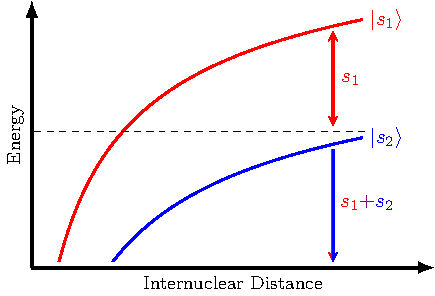
\includegraphics[width=0.7\textwidth]{figures/raman_spectroscopy_spin_mixing.pdf}
  \caption[Spin state mixing near the atomic threshold.]{
    Spin state mixing near the atomic threshold.
    Energy above the $s_2$ threshold only supports one molecular spin state
    so the bound state within the $s_1$ potential in this region is
    almost purely $s_1$.
    Energy below the $s_2$ threshold supports both $s_1$ and $s_2$ molecular states
    so bound states in this region may have a mixture of $s_1$ and $s_2$
    if the two spin states are coupled.
    This includes all the $s_2$ bound states and some of the $s_1$ bound states.
    \label{fig:raman-spectroscopy:spin-mixing}}
\end{figure}

Note that the Zeeman shift for the $|Na(2, 2),Cs(4, 4)\rangle$ state
is signicantly smaller than that for other spin states.
The reason for this is the magnetic coupling between the spin states
that has the same total $m_F$\footnote{The same coupling that leads to spin exchange collision.}.
The $|Na(2, 2),Cs(3, 3)\rangle$ spin state is coupled to the $|Na(2, 2),Cs(4, 3)\rangle$,
$|Na(1, 1),Cs(4, 4)\rangle$ and $|Na(2, 1),Cs(4, 4)\rangle$ states
whereas $|Na(1, 1),Cs(3, 3)\rangle$ is coupled to the $|Na(2, 1),Cs(3, 3)\rangle$,
$|Na(1, 1),Cs(4, 3)\rangle$, $|Na(2, 1),Cs(4, 3)\rangle$, $|Na(2, 2),Cs(3, 2)\rangle$
and $|Na(2, 2),Cs(4, 2)\rangle$ states.
All of these states listed above has higher energy so their bound states
may cause spin mixing with the $|Na(2, 2),Cs(3, 3)\rangle$ and $|Na(1, 1),Cs(3, 3)\rangle$
bound states (Fig.~\ref{fig:raman-spectroscopy:spin-mixing})
causing them to have a different magnetic field dependency from the corresponding atomic state
resulting in a non-zero differential Zeeman shift.
On the other hand, the $|Na(2, 2),Cs(4, 4)\rangle$ bound state is above
all the other spin states and therefore has a mostly pure spin state
and the transition has little Zeeman shift.

\section{Angular momentum Coupling in $N=2$ Ground State}
\label{ch:raman-spectroscopy:n2}

\todo{
  N=2 bound states/field dependency
}
\todo{
  (NaCs 2017-2018 > NaCs 2018 > Raman transfer 10/5 - 10/8 > v=-1 N=2 properties 11/03 - 11/07)
}

% Coherent optical creation of NaCs molecule
% -*- mode: latex-mode; TeX-engine: xetex; LaTeX-command-style: (("" "SOURCE_DATE_EPOCH=0 %(PDF)%(latex) --shell-escape %S%(PDFout)")); TeX-master: "../dissertation.tex"; -*-

\chapter{Coherent Optical Creation of NaCs Molecule}
\label{ch:raman-transfer}

\section{Introduction}
\label{ch:raman-transfer:introduction}

The coherent production of weakly bound ground state NaCs molecule is an important milestone
in our two-step approach of creating rovibronic ground state molecules with full control.
Achieving this goal using only optical transition without a narrow excited state linewidth
can allow more laser-coolable atoms to be associated to molecules coherently.
With the characterization of both the excited and ground molecular potential,
we have calibrated all the parameters needed to drive such a transition.
Nevertheless, the wavefunction size mismatch between the atomic and molecular states
remains a challenge that requires careful selection of the transition pathway.

In this chapter, we will discuss the considerations behind our choice of parameters
and show the result of the coherent molecule creation.
We begin with section~\ref{ch:raman-transfer:raman} to setup a model
for a realistic Raman transition beyond the ideal three-level system.
Section~\ref{ch:raman-transfer:stirap} follows a similar track and constructs a model
for stimulated Raman adiabatic passage~(STIRAP),
which is another common way to drive such a two-photon transition
and comparing it to the Raman transition.
Section~\ref{ch:raman-transfer:state-selction} uses the result from the previous sections
to finalize our molecule creation pathway.
The result of the molecule creation is given in section~\ref{ch:raman-transfer:results},
which also includes discussion on the transfer efficiency.

\section{Raman Transition Beyond Three-Level Model}
\label{ch:raman-transfer:raman}

For a Raman transition with Raman Rabi frequency $\Omega_{\mathrm{R}}$ and total scattering rate
$\Gamma$, defined as the sum of the scattering rate for the initial and final states,
the probability of scattering during a $\pi$ pulse is,
\begin{align*}
  p_{\mathrm{s}}=&\frac{\Gamma t_{\pi}}{2}\\
  =&\frac{\pi\Gamma}{2\Omega_{\mathrm{R}}}
\end{align*}
which is proportional to the ratio $\Gamma/\Omega_{\mathrm{R}}$.
In an ideal three-level system, this is the only source of decoherence
which can be made arbitrarily small by using a large
single photon detuning~(section~\ref{ch:rsc:basic-theory:raman-scatter}).
However, in a real system, there are often other effects that increases the scattering
and may also put a lower limit on the scattering probability during the transfer.
Fig.~\ref{fig:raman-transfer:generic-raman-model} shows a generic model
for a real Raman transition demostrating some of these effects.
Additionally, other practical limitation in the system like stability of the laser power
and frequency also needs to be taken into account.

\begin{figure}
  \centering
  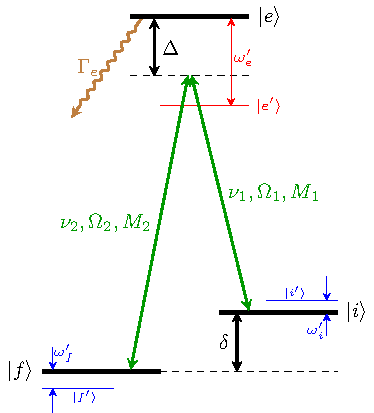
\includegraphics[width=0.6\textwidth]{figures/raman_transfer_generic_raman_model.pdf}
  \caption[Generic model for a real Raman transition]{
    Generic model for a real Raman transition.
    The initial state $|i\rangle$ and the final state $|f\rangle$
    has a energy difference $\delta$
    and are coupled by two Raman beams with frequencies and
    single photon Rabi frequencies of $\nu_1,\ \Omega_1$ and $\nu_2,\ \Omega_2$ respectively.
    The corresponding matrix elements (arbitrary unit) are $M_1$ and $M_2$.
    The Raman beams are detuned by $\Delta$ from the primary excited state $|e\rangle$,
    which has a decay rate of $\Gamma_e$.
    We also consider additional states near the initial~($|i'\rangle$),
    final~($|f'\rangle$) and intermediate excited $|e'\rangle$ states which are
    separated from the corresponding Raman transition states by $\omega'_i$,
    $\omega'_f$ and $\omega'_e$ respectively.
    Only one additional state of each kinds are included to simplify the discussion
    without loss of generality.
    \label{fig:raman-transfer:generic-raman-model}}
\end{figure}

In the experiment, we find the parameter range that gives the best transfer efficiency
using numerical simulation~(section~\ref{ch:raman-transfer:state-selction}).
Nevertheless, in order to develop a general approach that can be applied to other systems,
it is also important to understand the various physical mechanism that leads
to the optimal parameters.
Therefore, in this section, we will discuss some of the most important effects
on the transfer efficiency at qualitative and semiquantitative level.
Due to experimental constraint, we will assume that the single photon detuning is
much smaller than the frequency of each individual beams, i.e. $\Delta\ll\nu_1,\ \nu_2$.

\subsection{Additional Initial and Final States}
\label{ch:raman-transfer:raman:extra-init-final}

First, we will discuss the effect of $|i'\rangle$ and $|f'\rangle$ states
near the initial and final states.
These states can be coupled to the excited state $|e\rangle$ by the Raman beams,
which can in tern be coupled to the initial and final states
by an off-resonance Raman transition.
The leakage is suppressed by the detuning from the Raman resonance,
i.e. $\omega'_i$ and $\omega'_f$.
This puts a limit on the Raman Rabi frequency $\Omega_{\mathrm{R}}$ to be smaller
than the smallest energy gap, which in turns puts a limit on the minimum Raman transfer time.
In our experiment, the minimum energy gap comes from axial motional excitation of
the atomic initial states which is between $2\pi\times10 - 30~\mathrm{kHz}$
depending on the trap depth used.
The typical Raman $\pi$ time we can realize is $0.5 - 5~\mathrm{ms}$ so this effect
is not a major limiting factor for our transfer efficiency.

\subsection{Additional Excited States}
\label{ch:raman-transfer:raman:extra-ext}

\begin{figure}
  \centering
  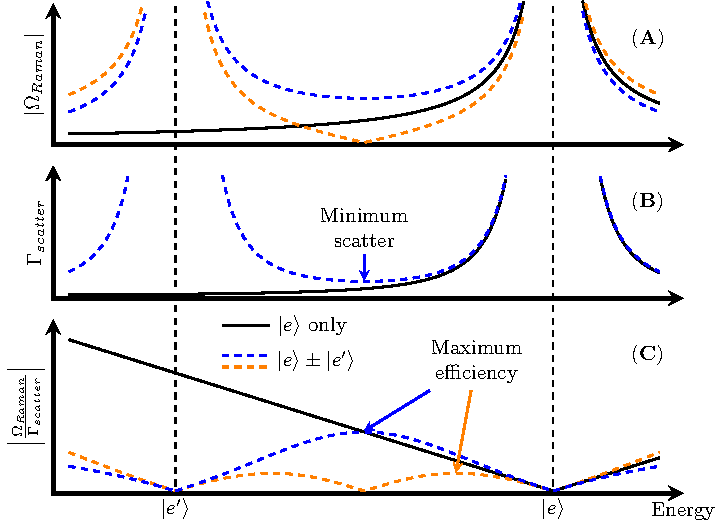
\includegraphics[width=\textwidth]{figures/raman_transfer_extra_ext_states.pdf}
  \caption[Raman transition with additional excited states]{
    Effect of additional excited states $|e'\rangle$ on the Raman transition efficiency.
    (A) Depending on the sign of the coupling, there could be constructive~(blue)
    or destructive~(orange) interference on the Raman Rabi frequency $\Omega_{\mathrm{R}}$.
    (B) Increased scattering rate $\Gamma_{\mathrm{s}}$ caused by $|e'\rangle$ with a minimal
    between the two states.
    (C) Optimal detunine exists between the two states with maximum transfer efficiency
    corresponds to a fraction of the state spacing.
    \label{fig:raman-transfer:raman:extra-ext-states}}
\end{figure}

Next, we will consider the effect of the $|e'\rangle$ state near the excited intermediate state.
These states can be coupled to the ground states, both $|i\rangle$ and $|f\rangle$,
by the Raman beams and can cause a change in both the Raman Rabi frequency
and the scattering rate.
There are two relevant limiting cases that needs to be discussed separately.

\subsubsection{Excited State Spacing Larger than Single-Photon Detuning}
\label{ch:raman-transfer:raman:extra-ext:large-spacing}
In this case, the single photon frequency falls in between the two excited states
$|e\rangle$ and $|e'\rangle$,
which happens when $|e'\rangle$ is a different vibrational or electronic state.
The total Raman Rabi frequency~(Fig.~\ref{fig:raman-transfer:raman:extra-ext-states}A) is,
\[
  \Omega_{\mathrm{R}}=\frac{\Omega_1\Omega_2}{2\Delta}+\frac{\Omega'_1\Omega'_2}{2(\Delta-\omega'_e)}
\]
where $\Omega'_1$ and $\Omega'_2$ are the single photon Rabi frequencies coupling $|e'\rangle$
to $|i\rangle$ and $|f\rangle$ respectively.
Depending on whether $\Omega'_1\Omega'_2$ has the same~(orange line)
or different~(blue line) sign as $\Omega_1\Omega_2$, the total Raman Rabi frequency
may be cancelled or enhanced between the two excited states.
On the other hand,
the total scattering rate~(Fig.~\ref{fig:raman-transfer:raman:extra-ext-states}B)
is almost always increased due to the additional state, creating a local minimum
between the excited states.
Combining the two effects, the ratio between the Raman Rabi frequency and
the scattering rate, which determines the transfer efficiency, always have local maximum
between the excited states~(Fig.~\ref{fig:raman-transfer:raman:extra-ext-states}C).

Despite the difference in the position and value of the maximum for different
$|e'\rangle$ parameters, we can summarize the effect on the transfer efficiency
as a limit on the maximum detuning $\Delta_{\max}$ to a fraction of the spacing
between the excited states~($\omega'_e$).
As an example, the blue and orange maxima in
Fig.~\ref{fig:raman-transfer:raman:extra-ext-states}C
corresponds to a limit on single photon detuning of $0.5\omega'_e$ and $0.15\omega'_e$.
As one would expected, a larger excited state spacing usually result in
a larger detuning limit and a better transfer efficiency.

Summarizing the effect of additional excited state as a single number $\Delta_{\max}$ allows
us to keep using the equation for Raman transition with minor corrections
and makes it easier to compare different state selection and transition schemes.
It is also worth noting that although only one additional excited state $|e'\rangle$
is considered here, this result can be generalized when more excited states are taken into account
as well. These states introduces additional smooth variation in both the Raman Rabi frequency
and scattering rate and the effects on the final transition efficiency can be similarly
treated as a change in the maximum detuning.

\subsubsection{Excited State Spacing Much Smaller than Single-Photon Detuning}
\label{ch:raman-transfer:raman:extra-ext:tight-spacing}
This is typically the case when $|e'\rangle$ is a different rotational or hyperfine state.
In this case, the Raman transition is detuned from both $|e\rangle$ and $|e'\rangle$
at the same time and the two excited states behaves similar to an effective state $|e''\rangle$
with modified coupling strengths and decay rate.

When the initial and final ground states have (nearly) identical spin and rotational state,
which is the case for the our transition to $N=0$ states
discussed in section~\ref{ch:raman-spectroscopy:states:n0},
the new effective state will behave very similar to the original ones.
This is because the coupling between the ground states and excited states is determined by,
\begin{align*}
  \Omega_{1,2}^{i}=&\Omega_{1,2}^{0}\langle\mathrm{F}_e^i|\mathrm{F}_g\rangle
\end{align*}
where the superscript $i$ represents different excited states,
the subscript $1,2$ represents the initial~(1) and final~(2) ground state,
$\Omega_{1,2}^{0}$ is the reduced Rabi frequency without the angular momentum projection,
and $\mathrm{F}_e^i$ and $\mathrm{F}_g$ are the rotation and spin state for the excited
and ground state respectively. Note that the ground states $|i\rangle$ and $|f\rangle$
both have the same $\mathrm{F}_g$. This means
\begin{align*}
  \frac{\Omega_1^{i}}{\Omega_2^{i}}=&\frac{\Omega_1^{0}}{\Omega_2^{0}}
\end{align*}
which is a constant.
Given that the excited state linewidth for different rotation and hyperfine states
are very similar, we have the Rabi frequency to scattering rate ratio.
\begin{align*}
  \frac{\Omega_{\mathrm{R}}}{\Gamma_{\mathrm{s}}}\approx&\paren{\sum_i\frac{\Omega_1^i\Omega_2^i}{2\Delta}}\left/\paren{\sum_i\frac{{\Omega_1^i}^2+{\Omega_2^i}^2}{4\Delta^2}}\right.\\
  =&\frac{\Omega_1\Omega_2}{2\Delta}\left/\frac{{\Omega_1}^2+{\Omega_2}^2}{4\Delta^2}\right.
\end{align*}
which is the same as the expression for a single excited state.

The properties of the effective state can be very different, however,
when the initial and final spin and rotational states are different.
Nevertheless, other than the special case of complete destructive interference
on the Raman Rabi frequency,
the new excited state will generally have a worse ratio $\Omega_{\mathrm{R}}/\Gamma_{\mathrm{s}}$
by a constant factor.
The dependency of the ratio on the detuning is not changed significantly
for large detuning.

\subsection{Cross Coupling Between Light Addressing Initial and Final States}
\label{ch:raman-transfer:raman:cross-couple}

Due to the small energy separation between the initial and final state $\delta$,
the cross coupling of the laser addressing the initial/final state on the final/initial state
is another important effect in our experiment.
Without the cross coupling, the total off resonance scattering rate for
the initial and the final states is
\[
  \Gamma_{\mathrm{s}0}=\frac{\Gamma_e\left(\Omega_1^2+\Omega_2^2\right)}{4\Delta^2}
\]
For a given Raman Rabi frequency $\Omega_{\mathrm{R}}\propto\Omega_1\Omega_2$, this is
minimized when $\Omega_1=\Omega_2$.

When cross coupling is taken into account, however, the total scattering rate becomes,
\footnote{Here we assume that the matrix elements are the same for the two beams.
  This is the case when the two beams have the same polarization as in our experiment.
  This effect can be minimized or eliminated by selecting different polarizations for the
  two laser frequencies that does not couple to the other initial/final state.
  This would also require choosing an excited state with the same or lower angular momentum
  as the ground states in order to avoid cross coupling to different excited states.}
\begin{align}
  \Gamma_{\mathrm{s}}=&\frac{\Gamma_e\Omega_1^2}{4M_1^2}\left(\frac{M_1^2}{\Delta^2}+\frac{M_2^2}{(\Delta+\delta)^2}\right)+\frac{\Gamma_e\Omega_2^2}{4M_2^2}\left(\frac{M_2^2}{\Delta^2}+\frac{M_1^2}{(\Delta-\delta)^2}\right)\\
  \propto&\frac{\Gamma_eP_1}{4}\left(\frac{M_1^2}{\Delta^2}+\frac{M_2^2}{(\Delta+\delta)^2}\right)+\frac{\Gamma_eP_2}{4}\left(\frac{M_2^2}{\Delta^2}+\frac{M_1^2}{(\Delta-\delta)^2}\right)
\end{align}
where $P_{1,2}\propto\Omega_{1,2}^2/M_{1,2}^2$ are the powers of the laser beams 1 and 2.
When $\delta\ll\Delta$ such as our experiment,
\begin{align*}
  \Gamma_{\mathrm{s}}\approx&\frac{\Gamma_e\left(M_1^2+M_2^2\right)}{4\Delta^2}\left(\frac{\Omega_1^2}{M_1^2}+\frac{\Omega_2^2}{M_2^2}\right)\\
  \propto&\frac{\Gamma_e\left(M_1^2+M_2^2\right)}{4\Delta^2}\left(P_1+P_2\right)
\end{align*}
For a given Raman Rabi frequency $\Omega_{\mathrm{R}}\propto\Omega_1\Omega_2\propto\sqrt{P_1P_2}$,
this is minimized when $P_1=P_2$.
Hence, due to the strong cross coupling, we need to use the same power in both Raman beams
rather than adjusting the powers to match their single photon Rabi frequencies.

Moreover, at the minimum scattering rate, we have $\Omega_2=\Omega_1M_2/M_1$
and the ratio between Raman Rabi frequency and scattering rate is,
\begin{align*}
  \frac{\Omega_{\mathrm{R}}}{\Gamma_{\mathrm{s}}}=&\frac{\Omega_1\Omega_2}{2\Delta}\frac{4\Delta^2}{\Gamma_e\left(M_1^2+M_2^2\right)}\left/\left(\frac{\Omega_1^2}{M_1^2}+\frac{\Omega_2^2}{M_2^2}\right)\right.\\
  =&\frac{2\Delta\Omega_1\Omega_2}{\Gamma_e\left(M_1^2+M_2^2\right)}\left/\left(\frac{\Omega_1^2}{M_1^2}+\frac{\Omega_2^2}{M_2^2}\right)\right.\\
  =&\frac{\Delta\Omega_1^2M_2}{\Gamma_eM_1\left(M_1^2+M_2^2\right)}\frac{M_1^2}{\Omega_1^2}\\
  =&\frac{\Delta}{\Gamma_e}\frac{M_1M_2}{M_1^2+M_2^2}
\end{align*}
Therefore, for a given excited state linewidth $\Gamma_e$
and maximum detuning~(section~\ref{ch:raman-transfer:raman:extra-ext}) the transfer efficiency
maximizes for the smallest $M_1M_2/(M_1^2+M_2^2)$ which happens when the ratio
$M_1/M_2$ is the closest to $1$.

The light shift of the Raman resonance is similarly affected by the cross coupling.
The differential light shift between the initial and the final state determines
the resonance fluctuation as a function of light intensity fluctuation.
The ration between the light shift and the Raman Rabi frequency, i.e. line width,
determines the stability requirement of our laser indensity.
With cross coupling, the differential shift is (assuming $\delta\ll\Delta$),
\begin{align*}
  \Delta\delta\approx&\frac{\Omega_1^2}{4\Delta}-\frac{\Omega_1^2M_2^2}{4\Delta M_1^2}-\frac{\Omega_2^2}{4\Delta}+\frac{\Omega_2^2M_1^2}{4\Delta M_2^2}\\
  =&\frac{M_1^2-M_2^2}{4\Delta}\left(\frac{\Omega_1^2}{M_1^2}+\frac{\Omega_2^2}{M_2^2}\right)\\
  \propto&\frac{M_1^2-M_2^2}{4\Delta}\left(P_1+P_2\right)
\end{align*}
which is also minimized when $P_1=P_2$ at a given Raman Rabi frequency.

The ratio with the Raman Rabi frequency is,
\begin{align*}
  \frac{\Delta\delta}{\Omega_{\mathrm{R}}}\approx&\frac{M_1^2-M_2^2}{4\Delta}\left(\frac{\Omega_1^2}{M_1^2}+\frac{\Omega_2^2}{M_2^2}\right)\frac{2\Delta}{\Omega_1\Omega_2}\\
  =&\frac{M_1^2-M_2^2}{2\Omega_1\Omega_2}\left(\frac{\Omega_1^2}{M_1^2}+\frac{\Omega_2^2}{M_2^2}\right)\\
  =&\frac{M_1^2-M_2^2}{M_1M_2}
\end{align*}
the absolute value of which is also minimized when the ratio $M_1/M_2$ is the closest to $1$.

Due to the coupling strength difference, we have $M_2\gg M_1$ in our experiment, which means,
\begin{align*}
  \left|\frac{\Delta\delta}{\Omega_{\mathrm{R}}}\right|\approx&\frac{M_2}{M_1}
\end{align*}
In order to keep the resonance stable within the linewidth of the Raman resonance,
i.e. $\Omega_{\mathrm{R}}$, we need to maintain a relative stability of $\Delta\delta$,
therefore relative stability of the laser power to better than $M_1/M_2$.

\section{STIRAP}
\label{ch:raman-transfer:stirap}

An alternative method often used to create and prepare the internal states of ultracold molecule
is stimulated Raman adiabatic passage~(STIRAP)~\cite{vitanov_coherent_2001}.
Compared to Raman transition, which uses detuning from the excited state
to reduce scattering during the transfer, STIRAP relies on a superposition between
the initial and final state as a dark state to achieve the same goal.
The dark state in STIRAP is created due to a destructive interference of transition
from the initial and final state to the excited state.

Similar to Raman transfer, STIRAP in an ideal three-level system can achieve
full coherent transfer with arbitrarily small scattering probability
when given unlimited time and power budget.
However, in reality, states and coupling that exist outside the ideal three-level system
always cause a non-zero probability of
scattering loss~(Fig.~\ref{fig:raman-transfer:generic-stirap-model}).
In this section, we will apply the approach we took for Raman transition to STIRAP.
We will then compare the loss caused by different practical limitations
and discuss which approach should be taken under certain circumstance.

\begin{figure}
  \centering
  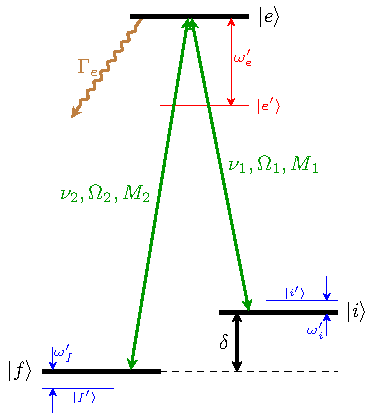
\includegraphics[width=0.6\textwidth]{figures/raman_transfer_generic_stirap_model.pdf}
  \caption[Generic model for a real STIRAP]{
    Generic model for a real STIRAP similar to Fig.~\ref{fig:raman-transfer:generic-raman-model}.
    Differences are that the two beams are now on resonant with $|e\rangle$
    and the $\Omega_1$ and $\Omega_2$ now represent the maximum single photon Rabi frequency
    during the STIRAP pulse for the two beams.
    \label{fig:raman-transfer:generic-stirap-model}}
\end{figure}

\subsection{STIRAP for Ideal Three-Level System}
\label{ch:raman-transfer:stirap:three-level}

During STIRAP, the system approximately remains in a dark state $|D(t)\rangle$
\begin{align*}
  |D(t)\rangle=&c_i(t)|i\rangle+c_f(t)|f\rangle
\end{align*}
Since this state does not couple to the excited state, we have,
\begin{align*}
  0=&\langle e|\mathbf{d}\cdot\mathbf{E}|D(t)\rangle\\
  =&c_i(t)\langle e|\mathbf{d}\cdot\mathbf{E}|i\rangle
     +c_f(t)\langle e|\mathbf{d}\cdot\mathbf{E}|f\rangle\\
  =&c_i(t)\Omega_1(t)+c_f(t)\Omega_2(t)
\end{align*}
or
\begin{align*}
  |D(t)\rangle=&\frac{\Omega_2(t)|i\rangle-\Omega_1(t)|f\rangle}{\sqrt{\Omega_1^2(t)+\Omega_2^2(t)}}
\end{align*}
In order to estimate the scattering rate,
we use the fact that the wavefunction amplitude in the final state $c_f$
is the integral of the excited state amplitude $c_e$ and the down leg Rabi frequency $\Omega_2$,
i.e.,\footnote{This equation and the lower bound on scattering probability applies generically
  to all two photon transfer process including Raman $\pi$ pulse.
  The equation we used in section~\ref{ch:raman-transfer:raman} is a refinement
  on this limit.}
\begin{align*}
  c_f(t)=&\int_0^t \frac{\ui\Omega_2(t)}{2}c_e(t') \ud t'
\end{align*}
For a complete transfer of length $T$, we have $c_f(0)=0$ and $c_f(T)=1$, therefore,
\begin{align*}
  \int_0^T\Omega_2(t)c_e(t)\ud t=&-2\ui
\end{align*}
Since $\Omega_2$ is the upper bound of $\abs{\Omega_2(t)}$ we have,
\begin{align*}
  \abs{\int_0^Tc_e(t)\ud t}\geqslant&\frac{2}{\Omega_2}
\end{align*}
The total scattering probability is,
\begin{align*}
  p_{\mathrm{s}0}=&\int_0^T \Gamma_e|c_e^2(t)| \ud t\\
  \geqslant&\frac{\Gamma_e}{T}\abs{\int_0^T c_e(t) \ud t}^2\\
  \geqslant&\frac{4\Gamma_e}{\Omega_2^2T}
\end{align*}
From similar argument, we also have,
\begin{align*}
  p_{\mathrm{s}0}\geqslant&\frac{4\Gamma_e}{\Omega_1^2T}
\end{align*}
which is the same as the previous result for a three-level STIRAP system
where $\Omega_1=\Omega_2$.
In the generic case, these give us a lower bound on the scattering probability,
\begin{align*}
  \min\paren{p_{\mathrm{s}0}}=&\frac{4\Gamma_e}{\min\paren{\Omega_1^2, \Omega_2^2}T}
\end{align*}
whereas the full scattering is larger than this lower bound by a pulse shape dependent
small constant factor.
It is also easy to verify that this result agrees with the scattering probability for
a optimal three-level Raman $\pi$ with similar single photon Rabi frequency and pulse time.
This confirms that without additional constraint from the real system or the experimental setup,
neither Raman transfer or STIRAP offers a significant advantage over the other.
As we will see in the following sections,
other effects in the system can favor one approach over the other one.

\subsection{Additional Initial and Final States}
\label{ch:raman-transfer:stirap:extra-init-final}

Similar to Raman transition~(section~\ref{ch:raman-transfer:raman:extra-init-final}),
the additional initial and final states causes potential leakage out of the three-level system.
This limits the minimum time of the transfer in a way similar to that of Raman transition.

\subsection{Additional Excited States}
\label{ch:raman-transfer:stirap:extra-ext}

For additional excited states that are farther away than the single photon Rabi frequency
$\Omega_1$ and $\Omega_2$, the contribution to the coherent transfer is minimum.
However, these states can still contribute to scattering during the transfer.

Excited state will only contribute significantly to the scattering if it causes scattering
from the dark state, which happens if $\Omega_1(t)/\Omega_2(t)\neq\Omega'_1(t)/\Omega'_2(t)$,
where $\Omega'_1(t)$ and $\Omega'_2(t)$ are the time dependent single photon Rabi frequencies
coupling $|e'\rangle$ to $|i\rangle$ and $|f\rangle$ respectively.
As discussed in section~\ref{ch:raman-transfer:raman:extra-ext:tight-spacing},
this does not happen for excited state with the same vibrational and electronic states
when the initial and final spin and rotational states are identical.
Similar to $\Omega_1$ and $\Omega_2$, we can also define
$\Omega'_1\equiv\max\paren{\Omega'_1(t)}$ and $\Omega'_2\equiv\max\paren{\Omega'_2(t)}$.
Since $\Omega'_1(t)$($\Omega'_2(t)$) and $\Omega_1(t)$($\Omega_2(t)$)
are generated from the same beam, we have
$\Omega'_1(t)\propto\Omega_1(t)$($\Omega'_2(t)\propto\Omega_2(t)$)
and the condition can also be equivalently expressed as
$\Omega_1/\Omega_2\neq\Omega'_1/\Omega'_2$.

More quantitatively,
the Rabi frequency coupling the dark state $|D(t)\rangle$ to the excited state $|e'\rangle$ is,
\begin{align*}
  \Omega'(t)=&\langle e'|\mathbf{d}\cdot\mathbf{E}|D(t)\rangle\\
  =&\frac{\Omega_2(t)\Omega'_1(t)-\Omega_1(t)\Omega'_2(t)}{\sqrt{\Omega_1^2(t)+\Omega_2^2(t)}}\\
  =&\frac{\Omega_1(t)\Omega_2(t)}{\sqrt{\Omega_1^2(t)+\Omega_2^2(t)}}\paren{\frac{\Omega'_1}{\Omega_1}-\frac{\Omega'_2}{\Omega_2}}
\end{align*}
The addtional scattering caused by this is,
\begin{align*}
  p'_{\mathrm{s}}=&\int_0^T \frac{\Gamma'_e\Omega'^2(t)}{4{\omega'_e}^2} \ud t\\
  =&\frac{\Gamma'_e}{4{\omega'_e}^2}
     \paren{\frac{\Omega'_1}{\Omega_1}-\frac{\Omega'_2}{\Omega_2}}^2
     \int_0^T \frac{\Omega_1^2(t)\Omega_2^2(t)}{\Omega_1^2(t)+\Omega_2^2(t)} \ud t\\
  =&C'\frac{\Gamma'_eT}{4{\omega'_e}^2}
     \paren{\frac{\Omega'_1}{\Omega_1}-\frac{\Omega'_2}{\Omega_2}}^2
     \frac{\Omega_1^2\Omega_2^2}{\Omega_1^2+\Omega_2^2}
\end{align*}
which has the form of an off-resonance scattering probability.
$C'$ is a dimensionless number depending only on the pulse shape defined as
\begin{align*}
  C'\equiv&\frac{\Omega_1^2+\Omega_2^2}{\Omega_1^2\Omega_2^2T}\int_0^T \frac{\Omega_1^2(t)\Omega_2^2(t)\ud t}{\Omega_1^2(t)+\Omega_2^2(t)}
\end{align*}

It is worth noting that although there aren't two different cases similar to
the discussion for Raman transition in section~\ref{ch:raman-transfer:raman:extra-ext}
due to the lack of detuning in STIRAP,
the difference between excited states with different spacings may still play an important role
when comparing Raman transition to STIRAP.
This is discussed breifly at the end of
section~\ref{ch:raman-transfer:stirap:raman-vs-stirap:extra-ext}.

\subsection{Cross Coupling Between Light Addressing Initial and Final States}
\label{ch:raman-transfer:stirap:cross-couple}

As is the case for Raman transition~(section~\ref{ch:raman-transfer:raman:cross-couple}),
the coupling of each beam on the other initial or final state can cause increased scattering.
The total scattering probability caused by the cross coupling is
\footnote{Here we are making the same assumption of identical matrix elements for the two beams
  as the one we made for Raman transition in section~\ref{ch:raman-transfer:raman:cross-couple}.},
\begin{align*}
  p''_{\mathrm{s}}=&\int_0^T \frac{\Gamma_e\Omega_1^2(t)}{4M_1^2}\frac{M_2^2}{\delta^2}\abs{c_f(t)}^2+\frac{\Gamma_e\Omega_2^2(t)}{4M_2^2}\frac{M_1^2}{\delta^2}\abs{c_i(t)}^2 \ud t\\
  =&\frac{\Gamma_e}{4\delta^2}\int_0^T \frac{M_2^2}{M_1^2}\frac{\Omega_1^4(t)}{\Omega_1^2(t)+\Omega_2^2(t)}+\frac{M_1^2}{M_2^2}\frac{\Omega_2^4(t)}{\Omega_1^2(t)+\Omega_2^2(t)} \ud t\\
  =&\frac{\Gamma_eT}{4\delta^2}\paren{C''_1\frac{M_2^2}{M_1^2}\frac{\Omega_1^4}{\Omega_1^2+\Omega_2^2}+C''_2\frac{M_1^2}{M_2^2}\frac{\Omega_2^4}{\Omega_1^2+\Omega_2^2}}
\end{align*}
where $C''_1$ and $C''_2$ are two dimentionless numbers
depending only on the pulse shape defined as,
\begin{align*}
  C''_i\equiv&\frac{\Omega_1^2+\Omega_2^2}{\Omega_i^4T}\int_0^T \frac{\Omega_i^4(t) \ud t}{\Omega_1^2(t)+\Omega_2^2(t)}
\end{align*}

\subsection{Raman Transfer versus STIRAP}
\label{ch:raman-transfer:stirap:raman-vs-stirap}

As one may expect, the scattering probability and the efficiency of a STIRAP transfer
depends on the precise pulse shape used.
While it may be possible to construct a STIRAP pulse shape
with significantly different constant values,
we will focus our discussion on more traditional shapes and assume
$C''_1\approx C''_2\approx C'\approx1$.

We will compare the scattering probability during STIRAP to that of
Raman $\pi$ pulse in two limiting case depending on whether the contribution
from the additional excited or ground state are more significant.

\subsubsection{More Significant Contribution from Additional Excited State}
\label{ch:raman-transfer:stirap:raman-vs-stirap:extra-ext}

This is the case where excited state separation $\omega_e'$ is significantly smaller compared
to the ground state separation $\delta$.
By choosing an optimal pulse time, the minimum scattering probability for the STIRAP is,
\begin{align*}
  p_{\mathrm{s}}^{\mathrm{STIRAP}}\approx&2\sqrt{\frac{4\Gamma_e}{\min\paren{\Omega_1^2, \Omega_2^2}}\frac{\Gamma'_e}{4{\omega'_e}^2}\paren{\frac{\Omega'_1}{\Omega_1}-\frac{\Omega'_2}{\Omega_2}}^2\frac{\Omega_1^2\Omega_2^2}{\Omega_1^2+\Omega_2^2}}\\
  =&\frac{\sqrt{\Gamma_e\Gamma'_e}}{\omega'_e}
     \abs{\frac{\Omega'_1}{\Omega_1}-\frac{\Omega'_2}{\Omega_2}}
     \frac{2\max\paren{\Omega_1, \Omega_2}}{\sqrt{\Omega_1^2+\Omega_2^2}}\\
  \geqslant&\frac{\sqrt{\Gamma_e\Gamma'_e}}{\omega'_e}
             \abs{\frac{\Omega'_1}{\Omega_1}-\frac{\Omega'_2}{\Omega_2}}
\end{align*}
For Raman $\pi$ pulse,
\begin{align*}
  p_{\mathrm{s}}^{\mathrm{Raman}}=&\frac{\pi\Gamma}{2\Omega_{\mathrm{R}}}\\
  =&\frac{\pi}{2}\frac{\Gamma_e\paren{\Omega_1^2+\Omega_2^2}}{4\Delta_{\max}^2}
     \frac{2\Delta_{\max}}{\Omega_1\Omega_2}\\
  =&\frac{\pi\Gamma_e}{4\Delta_{\max}}\frac{\paren{\Omega_1^2+\Omega_2^2}}{\Omega_1\Omega_2}\\
  \geqslant&\frac{\pi\Gamma_e}{2\Delta_{\max}}
\end{align*}
The last inequality for both take the equal sign when $\Omega_1=\Omega_2$.
Comparing the result and note that $\Delta_{\max}$ is a fraction of $\omega_e'$,
we see that the two scales similarly to the excited state spacing.
However, given that in the common cases we have $\Delta_{\max}<\omega_e'$ and
$\abs{\Omega'_1/\Omega_1-\Omega'_2/\Omega_2}<1$ using STIRAP can potentially reduce
the total scattering in this case.

Note that the discussion above implicitly assumes that the relevant $\omega_e'$
is the same for Raman transition and STIRAP.
However, as we saw in section~\ref{ch:raman-transfer:stirap:extra-ext} and
\ref{ch:raman-transfer:raman:extra-ext:tight-spacing},
this may not be the case for hyperfine and rotational structure
in the excited state when the initial and final states have different spin states.
The $\omega_e'$ for STIRAP in this case is the hyperfine or rotational splitting
and may be significantly smaller compared to the $\omega_e'$ for Raman transition,
which is the vibrational state spacing.
As a result, STIRAP may not be as favorable compared to Raman anymore.
The best option in this case would require more in-depth comparison
of the different effects and will not be discussed here in more detail
since it is not relevant in our experiment.

\subsubsection{More Significant Contribution from Additional Ground State}
\label{ch:raman-transfer:stirap:raman-vs-stirap:cross-couple}

With the assumption of $C''_1\approx C''_2\approx1$ the scattering due to
cross coupling for STIRAP is now,
\begin{align*}
  p''_{\mathrm{s}}=&\frac{\Gamma_eT}{4\delta^2}\paren{\frac{M_2^2}{M_1^2}\frac{\Omega_1^4}{\Omega_1^2+\Omega_2^2}+\frac{M_1^2}{M_2^2}\frac{\Omega_2^4}{\Omega_1^2+\Omega_2^2}}\\
  \geqslant&\frac{\Gamma_eT}{2\delta^2}\paren{\Omega_1^2+\Omega_2^2}\frac{M_1^2M_2^2}{\paren{M_1^2+M_2^2}^2}
\end{align*}
and the minimum is taken when $M_2/M_1=\Omega_2/\Omega_1$\footnote{Same as Raman transition.}
The minimum total scattering rate for STIRAP is therefore,
\begin{align*}
  p_{\mathrm{s}}^{\mathrm{STIRAP}}\approx&2\sqrt{\frac{4\Gamma_e}{\min\paren{\Omega_1^2, \Omega_2^2}}\frac{\Gamma_e}{2\delta^2}\paren{\Omega_1^2+\Omega_2^2}\frac{M_1^2M_2^2}{\paren{M_1^2+M_2^2}^2}}\\
  =&2\sqrt{2}\frac{\Gamma_e}{\delta}\frac{M_1M_2}{M_1^2+M_2^2}\frac{\sqrt{\Omega_1^2+\Omega_2^2}}{\min\paren{\Omega_1, \Omega_2}}\\
  =&2\sqrt{2}\frac{\Gamma_e}{\delta}\frac{\max\paren{M_1, M_2}}{\sqrt{M_1^2+M_2^2}}\approx2\sqrt{2}\frac{\Gamma_e}{\delta}
\end{align*}
For Raman transition
\begin{align*}
  p_{\mathrm{s}}^{\mathrm{Raman}}=&\frac{\pi\Gamma}{2\Omega_{\mathrm{R}}}\\
  =&\frac{\pi\Gamma_e}{2\Delta}\frac{M_1^2+M_2^2}{M_1M_2}\\
  \approx&\frac{\pi\Gamma_e}{2\Delta}\frac{\max\paren{M_1,M_2}}{\min\paren{M_1,M_2}}
\end{align*}
we can see that when the single photon Rabi frequency is changed to minimize
cross coupling scattering, the Raman transition can be more strongly affected by
the matrix element imbalance. However, if the Raman transition can use a detuning
\[
  \Delta>\frac{\max\paren{M_1,M_2}}{\min\paren{M_1,M_2}}\delta
\]
then the scattering probability for a Raman transition can be made smaller than that of STIRAP.

\subsubsection{Conclusion}

In our experiment, we have an initial and final state separation of $< 1~\mathrm{GHz}$
and an matrix element ratio of $< 30$.
This means that as long as we can use a single photon detuning of more than
$\approx 30~\mathrm{GHz}$, the total scattering probability for Raman transition
will be smaller than that of STIRAP.
Since this detuning can be achieved easily,
a Raman $\pi$ pulse should be preferred in our experiment.

The comparison so far has been focused on the scattering probability from the Raman or STIRAP
beams. There are also a few other more technical reasons we preferred Raman versus STIRAP
in our experiment.

\begin{enumerate}
\item We use the tweezer beam as the Raman beam for transfer in order to reduce scattering
  from external sources~(section~\ref{ch:raman-spectroscopy:states}).
  Doing this for STIRAP while optimizing the pulse shape for transfer is more challenging.
\item In additional to scattering, the additional excited and ground state
  also causes a power, and therefore time, dependent light shift.
  A STIRAP in the presence of these shifts must vary the frequency of the two beams
  in additional to the power in order to maintain the dark state.
  This is also technically challenging to do.
\end{enumerate}

As a summary, for two photon transfer to a weakly bound molecular state,
it is likely that Raman transition is the preferred technique.
However, for transfering to a deeply bound molecular state,
which is where STIRAP is used in previous experiments,
STIRAP can have an advantage over Raman transition.

\section{States Selection}
\label{ch:raman-transfer:state-selction}

From section~\ref{ch:raman-transfer:raman} we see that the transfer efficiency
is directly related to the excited state linewidth, the maximum usuable detuning
and the matrix elements ratio~($M_1/M_2$).
In this section, we will discuss how these, as well as other technical constraints
affects the choices of states we use for the Raman transfer.

\subsection{Initial Atomic State}
\label{ch:raman-transfer:state-selction:init}

\begin{figure}
  \centering
  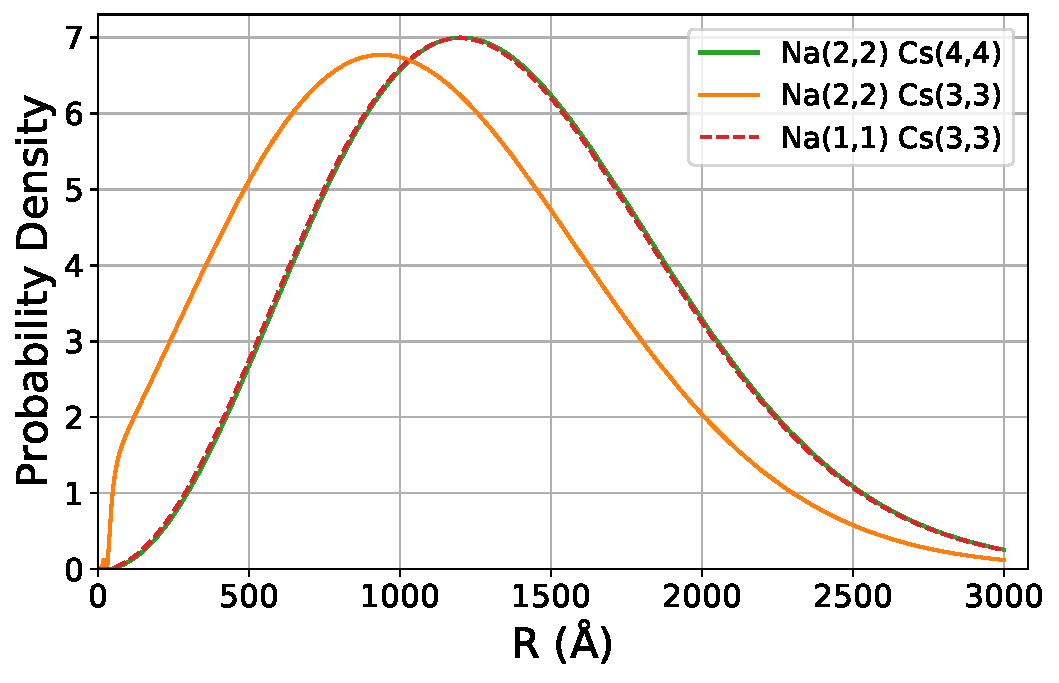
\includegraphics[width=0.625\textwidth]{figures/raman_transfer_atomic_wavefunction.pdf}
  \caption[Enhancement of short range wavefunction]{
    Enhancement of short range wavefunction.
    The large scattering length for the $\mathrm{Na(2,2),Cs(3,3)}$ state
    creates an interaction shift comparable to the axial trapping frequency.
    This causes a significant change in the relative wavefunction especially at short
    intranuclear distance~($R$).
    Compared to other spin states with weaker interaction,
    the wavefunction at short distance~($R<100~\text{\AA}$) is significantly enhanced.
    \label{fig:raman-transfer:atomic-wavefunction}}
\end{figure}

The choice of initial state can affect the transfer efficiency
by changing the matrix element $M_1$ and therefore the matrix elements ratio.
Since for most choices of the atomic and molecular states we have $M_1<M_2$,
we would like to choose an atomic initial state with the largest $M_1$ possible.
Unlike the selection of final state~(section~\ref{ch:raman-transfer:state-selction:final})
maximizing $M_1$ can improve the matrix element ratio as well as
shortening the transfer time to decrease sensitivity to technical noise at the same time.

As discussed in section~\ref{ch:pa:linewidth},
$M_1$ is only sensitive to the wavefunction at a short inter-atomic distance
that is comparable to the size of the molecule.
Therefore, states with a large wavefunction value at short inter-atomic distance
should generally have a larger $M_1$.
In additional to the confinement potential and the motional state of the atoms,
this is also affected by the interaction between the atoms.
A stronge interaction, either attractive or repulse,
can significantly change the relative motional wavefunction of the atoms.
This effect can be seen in Fig.~\ref{fig:raman-transfer:atomic-wavefunction}
and is especially significant for the $|\mathrm{Na(2,2),Cs(3,3)}\rangle$ state
when the interaction energy scale is comparable to that of the motional energy
as seen in section~\ref{ch:interaction-shift:spectroscopy:results}.

\subsection{Excited State}
\label{ch:raman-transfer:state-selction:ext}

\begin{figure}
  \centering
  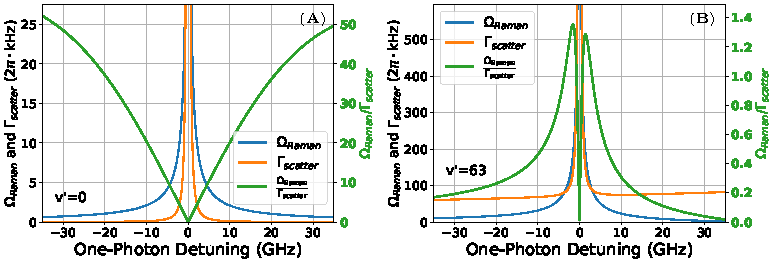
\includegraphics[width=\textwidth]{figures/raman_transfer_v0_vs_v63.pdf}
  \caption[Comparison between using a weakly bound and a deeply bound excited state
  as intermediate state for the Raman transition]{
    Comparison between using a weakly bound and a deeply bound excited state
    as intermediate state for the Raman transition.
    The (A) deeply bound excited state~($v'=0$) has a smaller
    Raman Rabi frequency`($\Omega_{\mathrm{R}}$) compared to the
    (B) weakly bound excited state~($v'=63$) at a given detuning.
    However, the lower scattering rate~($\Gamma_{\mathrm{s}}$) allows a much larger
    $\Delta_{\max}$,
    which results in a larger Raman Rabi frequency to scattering rate ratio.
    \label{fig:raman-transfer:v0-vs-v63}}
\end{figure}

Based on theory calculation, most of the molecular excited states have a linewidth $\Gamma_e'$
very similar to that of the Cesium D lines between $2\pi\times5~\mathrm{MHz}$ to
$2\pi\times10~\mathrm{MHz}$ due to optical decay process.
States above the Cesium $\mathrm{6^2P_{1/2}}$ state,
however, could non-radiatively decay to the Cs $\mathrm{6^2P_{1/2}}$
and Na $\mathrm{3^2S_{1/2}}$ states
via pre-dissociation which significantly increases the linewidth and should be avoided.

The other factor that affects excited state selection is the maximum detuning $\Delta_{\max}$.
Due to larger FCF with the ground atomic and weakly bound molecular state,
previous attempt at Raman spectroscopy typically use an excited state
closed to the dissociative threshold as
the intermediate state~\cite{wynar_molecules_2000,rom_state_2004}.
However, the smaller inter-state spacing and the smaller detuning from
the atomic excited state means that these state have a relatively small $\Delta_{\max}$
and therefore a lower coherent transfer efficiency.
On the other hand, a deeply bound excited state has a significantly higher $\Delta_{\max}$
and is the preferred choice for coherent Raman transfer.

In the experiment, we use numerical simulation to calculate the Raman transfer efficiency
for any given Raman beam wavelength taking into account of all states of
the $\mathrm{c^3\Sigma^+}(\Omega = 1)$
excited molecular state potential~\cite{grochola_spin-forbidden_2011}
and the continuum~\cite{liu_ultracold_2017}.
Fig.~\ref{fig:raman-transfer:v0-vs-v63} shows the result near a deeply bound
and weakly bound excited state.
Despite having a lower Raman Rabi frequency,
the deeply bound state has significantly higher transfer efficiency
and is used as the intermediate state for coherent Raman transfer in our experiment.

\subsection{Final Molecular State}
\label{ch:raman-transfer:state-selction:final}

In additional to the scattering and light shift considertions discussed above,
the transition can also be affected by external magnetic field.
We minimize the effect of magnetic field noise on the transition by using molcular
and atomic states that are in the same molecular potential,
i.e. molecular bound state in the potential that asymptote to
the atomic state. For weakly bound molecular state,
i.e. binding energy smaller than or comparable to the hyperfine energy scale,
this ensures that the atomic and molecular states has maximally overlapping spin state
and therefore a small differential Zeeman shift that can affect the Raman resonance frequency.
The similarity in the spin state between the initial and final states
also minimizes the effect of hyperfine and rotational states near the excited states
as we have seen in section~\ref{ch:raman-transfer:raman:extra-ext:tight-spacing}.

Because of the weak coupling between the atomic and molecular states,
the Raman transition has a relatively low Rabi frequency.
This also means a longer transfer time over which the Raman lasers must remain coherent.
In order to lower the requirement on our Raman and tweezer laser,
we select the first bound state, i.e. smallest binding energy, as the final molecular state.
This ensures the maximum Raman Rabi frequency.
Additionally, the typical binding energy for these states are $<1~\mathrm{GHz}$
which is a frequency difference that can be generated using AOM's
so that the coherence between the two beams is greatly improved.

\section{Raman Transfer Results}
\label{ch:raman-transfer:results}

The setup and sequence for forming the molecule is very similar to that of the Raman spectsocopy
previously mentioned in section~\ref{ch:raman-spectroscopy:states:raman-tweezer}
that drives the two-photon transition by adding a second frequency to the tweezer light.
Nevertheless, a few changes were made to the sequence in order to improve
the transfer efficiency and the signal to noise.
\begin{enumerate}
\item The initial $|\mathrm{Na(2,2),Cs(3,3)}\rangle$ state is prepared by driving the
  interaction shift resonance from $|\mathrm{Na(2,2),Cs(4,4)}\rangle$
  after the two atoms are merged into the same tweezer.
  As discussed in section~\ref{ch:interaction-shift:summary},
  the strong interaction between the atoms allows preparation of
  relative motional ground state with low background.
\item Instead of using smaller detuning and longer time to maximize the signal of the resonance,
  we increased the single photon detuning to $145~\mathrm{GHz}$
  and use short pulse times~($<1~\mathrm{ms}$)
  to reduce the scattering and the linewidth of the resonance.
\item We added an narrow bandpass filter to reduce the spectral noise from the laser.
  This will be discussed in more detail below.\todo{ref}
\end{enumerate}

With these changes, the narrowest linewidth we were able to observe using $15~\mathrm{mW}$
of total power in the tweezer is shown in Fig.~\todo{ref, data using one ASE filter}.
The full width half maximum~(FWHM) of $\todo{number}~\mathrm{kHz}$ is consistent
with the Fourier limited linewidth of $\todo{number}~\mathrm{kHz}$
for a $\pi$-pulse of $\todo{number}~\mathrm{ms}$ used in the experiment.
This is evidence that the linewidth is mainly determined by the Raman Rabi frequency
rather than the lifetime of the molecule, suggesting that we are in the coherent regime.
We can confirm this by varying the pulse time on the Raman resonance
and the resulting decaying Rabi flopping can be seen in Fig.~\todo{ref}.

\todo{
  Lower than expected efficiency
  Scan dependency of parameters to determine the cause
}

\subsection{Effect of laser spectral noise}
\label{ch:raman-transfer:results:ase}

\todo{define ASE}

\begin{figure}
  \centering
  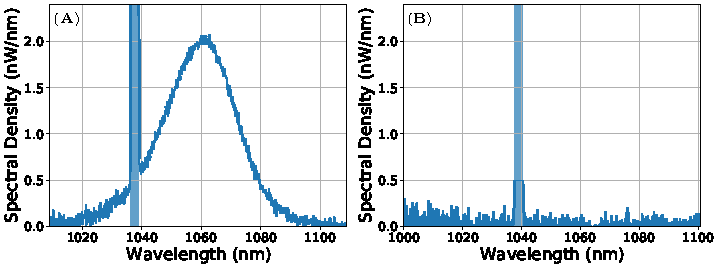
\includegraphics[width=\textwidth]{figures/raman_transfer_spectra.pdf}
  \caption[Tweezer spectra before and after ASE filter]{
    Spectra of the tweezer beam (A) before and (B) after the ASE filter.
    The power in the desired output frequency from the laser is $20\sim200~\mathrm{\mu W}$
    where the uncertainty is caused by saturation of the spectrum analyser.
    This saturated range is shown as the vertical blue bands in both plots.
    The exact position of this band depends on the scan setting
    which causes it to be slightly different between the two spectra.
    (A) The spectrum before the ASE filter clearly shows a broad band spectral impurity
    that spans tens of nm potentially covering multiple molecular excited states.
    (B) With the ASE filter, the spectrum is consistent with the background.
    \label{fig:raman-transfer:results:ase:spectra}}
\end{figure}

\ref{fig:raman-transfer:results:ase:spectra}

\subsection{Scaling of Raman Transition Parameters}
\label{ch:raman-transfer:results:scaling}

\todo{
  Types of sources: one/two photon
  Background/v=0 contribution
}

\section{Summary and Outlook}
\label{ch:raman-transfer:summary}

\todo{
  Reference loss due to coupling to atomic motional continuum
}


(outlook:)

Since the final state is mainly selected based on technical considerations,
there are other choices that can potentially improve the transfer efficiency.
As an exmple, states with larger binding energies can have weaker coupling
to the excited state therefore reducing the matrix elements ratio.
Doing so would likely require locking two lasers with a coherence time
longer than a few milliseconds.

% -*- mode: latex-mode; TeX-engine: xetex; LaTeX-command-style: (("" "SOURCE_DATE_EPOCH=0 %(PDF)%(latex) --shell-escape %S%(PDFout)")); TeX-master: "../dissertation.tex"; -*-

\chapter{Conclusion}
\label{conclusion}


\setstretch{\dnormalspacing}

% the back matter
\begin{appendices}
  % -*- mode: latex-mode; TeX-engine: xetex; LaTeX-command-style: (("" "SOURCE_DATE_EPOCH=0 %(PDF)%(latex) --shell-escape %S%(PDFout)")); TeX-master: "../dissertation.tex"; -*-

\chapter{Computer control appendex}
\label{appendex:computer-control}
(Hardware spec)

  % -*- mode: latex-mode; TeX-engine: xetex; LaTeX-command-style: (("" "SOURCE_DATE_EPOCH=0 %(PDF)%(latex) --shell-escape %S%(PDFout)")); TeX-master: "../dissertation.tex"; -*-

\chapter{Raman Sideband Cooling Appendex}
\label{appendex:rsc}

Each Raman pulse in the cooling sequence is followed immediately by an optical pumping pulse.
The full parameters for the Raman pulses, including the cooling ``axis'',
the sideband ``order ($\Delta n$)'', the cooling frequency ``$\delta '$",
the carrier ($\Delta n=0$) frequency ``$\delta_0'$'', the pulse ``duration'',
the pulse strength in ``$\Omega_0$'',
and the beam of which a non-uniform ``power ramp'' is applied, are listed in 6 groups below.
The applied cooling frequency, $\delta'$,
is the two-photon detuning given relative to the zero-field $F=1$ and $F=2$ hyperfine splitting
of $1.7716261288(10)$GHz~\cite{steck_sodium_nodate}.
Due to the Stark shifts of the Raman beams, the carrier transition, $\delta'_0$,
varies with the power of the Raman beams.
$\delta'_0$ is given also relative to the zero-field hyperfine splitting.
The strength of the pulses given in $\Omega_0$ determines the two-photon Rabi frequency,
$\Omega_{n,\Delta n}=\Omega_0 \langle n|e^{i \vec{k} \cdot \vec{r}}|n+\Delta n\rangle$.
We adopt the convention that a $\pi$-pulse between state $n$ and $n+\Delta n$ requires a duration $\pi/\Omega_{n,\Delta n}$.
The difference between $\delta'$ and $\delta'_0$ gives the motional sideband frequency, $\delta$.
Many Raman pulses include a ``power ramp'' with a Blackman envelope~\cite{kasevich_laser_1992} to minimize off-resonant excitations.
Because each Raman pulse is a product of two spatial- and temporal-overlapped laser beams,
the ``power ramp'' is applied only to the beam that has the smaller light shift
(we label the beam by the corresponding $F$ number) while the other beam has a square-pulse shape.
For a Raman pulse with a power ramp,
the Rabi frequency gives the arithmetic mean over the duration of the pulse.

\newpage

\subsubsection{Group 1}
This group is repeated 4 times.
\begin{center}
  \begin{tabular}{|c|c|c|c|c|c|c|}
    \hline
    Axis&$\Delta n$&$\delta'$ (MHz)&$\delta'_0$ (MHz)&Duration ($\mu$s)& $\Omega_0$ (kHz)&Power ramp\\\hline
    $x$&-2&$19.625$&$18.649$&44.1&$2\pi\times23$&F1\\\hline
    $y$&-2&$19.615$&$18.648$&28.6&$2\pi\times35$&F1\\\hline
    $x$&-1&$19.130$&$18.649$&36.9&$2\pi\times23$&F1\\\hline
    $y$&-1&$19.615$&$18.648$&24.0&$2\pi\times35$&F1\\\hline
  \end{tabular}
\end{center}

\subsubsection{Group 2}
This group is repeated 5 times.
\begin{center}
  \begin{tabular}{|c|c|c|c|c|c|c|}
    \hline
    Axis&$\Delta n$&$\delta'$ (MHz)&$\delta'_0$ (MHz)&Duration ($\mu$s)& $\Omega_0$ (kHz)&Power ramp\\\hline
    $z$&-5&$19.030$&$18.605$&81.5&$2\pi\times16$&F2\\\hline
    $x$&-2&$19.625$&$18.649$&44.1&$2\pi\times23$&F1\\\hline
    $z$&-4&$18.940$&$18.605$&76.3&$2\pi\times16$&F2\\\hline
    $y$&-2&$19.615$&$18.648$&28.6&$2\pi\times35$&F1\\\hline
    $z$&-5&$19.030$&$18.605$&81.5&$2\pi\times16$&F2\\\hline
    $x$&-1&$19.130$&$18.649$&36.9&$2\pi\times23$&F1\\\hline
    $z$&-4&$18.940$&$18.605$&76.3&$2\pi\times16$&F2\\\hline
    $y$&-1&$19.130$&$18.648$&24.0&$2\pi\times35$&F1\\\hline
  \end{tabular}
\end{center}
\subsubsection{Group 3}
This group is repeated 6 times.
\begin{center}
  \begin{tabular}{|c|c|c|c|c|c|c|}
    \hline
    Axis&$\Delta n$&$\delta'$ (MHz)&$\delta'_0$ (MHz)&Duration ($\mu$s)& $\Omega_0$ (kHz)&Power ramp\\\hline
    $z$&-4&$18.940$&$18.605$&76.3&$2\pi\times16$&F2\\\hline
    $x$&-2&$19.625$&$18.649$&44.1&$2\pi\times23$&F1\\\hline
    $z$&-3&$18.858$&$18.605$&70.2&$2\pi\times16$&F2\\\hline
    $y$&-2&$19.615$&$18.648$&28.6&$2\pi\times35$&F1\\\hline
    $z$&-4&$18.940$&$18.605$&76.3&$2\pi\times16$&F2\\\hline
    $x$&-1&$19.130$&$18.649$&36.9&$2\pi\times23$&F1\\\hline
    $z$&-3&$18.858$&$18.605$&70.2&$2\pi\times16$&F2\\\hline
    $y$&-1&$19.130$&$18.648$&24.0&$2\pi\times35$&F1\\\hline
  \end{tabular}
\end{center}

\newpage
\subsubsection{Group 4}
This group is repeated 7 times.
\begin{center}
  \begin{tabular}{|c|c|c|c|c|c|c|}
    \hline
    Axis&$\Delta n$&$\delta'$ (MHz)&$\delta'_0$ (MHz)&Duration ($\mu$s)& $\Omega_0$ (kHz)&Power ramp\\\hline
    $z$&-3&$18.858$&$18.605$&70.2&$2\pi\times16$&F2\\\hline
    $x$&-2&$19.625$&$18.649$&44.1&$2\pi\times23$&F1\\\hline
    $z$&-2&$18.773$&$18.605$&62.7&$2\pi\times16$&F2\\\hline
    $y$&-2&$19.615$&$18.648$&28.6&$2\pi\times35$&F1\\\hline
    $z$&-3&$18.858$&$18.605$&70.2&$2\pi\times16$&F2\\\hline
    $x$&-1&$19.130$&$18.649$&36.9&$2\pi\times23$&F1\\\hline
    $z$&-2&$18.773$&$18.605$&62.7&$2\pi\times16$&F2\\\hline
    $y$&-1&$19.130$&$18.648$&24.0&$2\pi\times35$&F1\\\hline
  \end{tabular}
\end{center}

\newpage
\subsubsection{Group 5}
This group is repeated 10 times.
\begin{center}
  \begin{tabular}{|c|c|c|c|c|c|c|}
    \hline
    Axis&$\Delta n$&$\delta'$ (MHz)&$\delta'_0$ (MHz)&Duration ($\mu$s)& $\Omega_0$ (kHz)&Power ramp\\\hline
    $z$&-2&$18.773$&$18.605$&62.7&$2\pi\times16$&F2\\\hline
    $x$&-1&$19.130$&$18.649$&36.9&$2\pi\times23$&F1\\\hline
    $z$&-1&$18.685$&$18.605$&52.5&$2\pi\times16$&F2\\\hline
    $y$&-1&$19.130$&$18.648$&24.0&$2\pi\times35$&F1\\\hline
    $z$&-2&$18.773$&$18.605$&62.7&$2\pi\times16$&F2\\\hline
    $x$&-1&$19.130$&$18.649$&70.0&$2\pi\times23$&F1\\\hline
    $z$&-1&$18.685$&$18.605$&52.5&$2\pi\times16$&F2\\\hline
    $y$&-1&$19.130$&$18.648$&46.0&$2\pi\times35$&F1\\\hline
  \end{tabular}
\end{center}

\newpage
\subsubsection{Group 6}
This group is repeated 30 times.
\begin{center}
  \begin{tabular}{|c|c|c|c|c|c|c|}
    \hline
    Axis&$\Delta n$&$\delta'$ (MHz)&$\delta'_0$ (MHz)&Duration ($\mu$s)& $\Omega_0$ (kHz)&Power ramp\\\hline
    $z$&-1&$18.683$&$18.605$&78.7&$2\pi\times11$&F2\\\hline
    $z$&-1&$18.683$&$18.605$&135.0&$2\pi\times11$&F2\\\hline
    $z$&-1&$18.685$&$18.605$&78.7&$2\pi\times11$&F2\\\hline
    $x$&-1&$19.130$&$18.649$&36.9&$2\pi\times23$&F1\\\hline
    $y$&-1&$19.130$&$18.648$&24.0&$2\pi\times35$&F1\\\hline
    $z$&-1&$18.685$&$18.605$&78.7&$2\pi\times11$&F2\\\hline
    $z$&-1&$18.685$&$18.605$&135.0&$2\pi\times11$&F2\\\hline
    $z$&-1&$18.685$&$18.605$&78.7&$2\pi\times11$&F2\\\hline
    $x$&-1&$19.130$&$18.649$&70.0&$2\pi\times23$&F1\\\hline
    $y$&-1&$19.130$&$18.648$&46.0&$2\pi\times35$&F1\\\hline
  \end{tabular}
\end{center}

\end{appendices}
% -*- mode: latex; TeX-engine: xetex; LaTeX-command-style: (("" "SOURCE_DATE_EPOCH=0 %(PDF)%(latex) --shell-escape %S%(PDFout)")); TeX-master: "../dissertation.tex"; -*-

\clearpage
\begin{spacing}{\dcompressedspacing}
  \bibliography{references/references}
  \addcontentsline{toc}{chapter}{References}
  \bibliographystyle{apalike2}
\end{spacing}

\end{document}
